% --- Encoding and base class ---
\documentclass[12pt]{article}
\usepackage[T1]{fontenc}
\usepackage[utf8]{inputenc}

% --- Geometry and typography ---
\usepackage[letterpaper,margin=1in]{geometry}
\usepackage[protrusion=true,expansion=true]{microtype} % 微排版优化
\usepackage{setspace}
\setstretch{1.12}
\addtolength{\parskip}{.45\baselineskip}

% --- Graphics & Colors ---
\usepackage{graphicx}
\usepackage{xcolor}
\usepackage{booktabs}
\usepackage{float}
\usepackage{tikz}
\usetikzlibrary{arrows.meta, cd} % TikZ-cd for commutative diagrams

% --- Math Packages (The Core) ---
\usepackage{amsmath,amssymb,amsthm}
\usepackage{mathtools} % 必须在 amsmath 之后
\usepackage{mathrsfs}  % 提供 \mathscr (用于 sigma-algebra, e.g., \mathscr{F})
\usepackage{esint}     % 提供 \fint (average integral) 等符号
\usepackage{bm}        % 粗体数学符号

% Math Tools Settings
% showonlyrefs: 仅给被引用的公式编号 (让笔记更干净)
% centercolon: 修正 := 的冒号垂直居中问题
\mathtoolsset{showonlyrefs,centercolon}
\numberwithin{equation}{section}

% --- Hyperlinks and References ---
\usepackage[pdfusetitle,unicode,psdextra]{hyperref}
\hypersetup{
  colorlinks=true,
  linkcolor=blue!60!black,
  citecolor=blue!60!black,
  urlcolor=blue!60!black,
  breaklinks=true
}
\usepackage[nameinlink,capitalize]{cleveref}

% --- Hyperref Bookmarks Fix (防止书签报错) ---
\pdfstringdefDisableCommands{
  \def\vect#1{#1}
  \def\abs#1{|#1|}
  \def\norm#1{||#1||}
  \def\eps{epsilon}
  \def\diff{d}
  \def\R{R}
}

% --- Lists and Algorithms ---
\usepackage{enumitem}
\setlist{itemsep=2pt,topsep=4pt}
\usepackage[ruled,vlined]{algorithm2e}

% --- Date format ---
\usepackage{datetime}
\newdateformat{mydate}{\THEDAY~\monthname[\THEMONTH] \THEYEAR}

% =========================================
%  Math Macros (Real Analysis Specific)
% =========================================

% 1. Number Systems & Sets
\newcommand{\RR}{\mathbb{R}}
\newcommand{\CC}{\mathbb{C}}
\newcommand{\QQ}{\mathbb{Q}}
\newcommand{\ZZ}{\mathbb{Z}}
\newcommand{\NN}{\mathbb{N}}
\newcommand{\FF}{\mathbb{F}}
\let\oldemptyset\emptyset
\let\emptyset\varnothing

% 2. Delimiters (使用 mathtools 的强大功能)
% 用法: \abs{x} (自动大小), \abs*{x} (自动调整), \abs[\big]{x} (手动)
\DeclarePairedDelimiter{\abs}{\lvert}{\rvert}
\DeclarePairedDelimiter{\norm}{\lVert}{\rVert}
\DeclarePairedDelimiter{\set}{\{}{\}}
\DeclarePairedDelimiter{\inner}{\langle}{\rangle}
\DeclarePairedDelimiter{\ceil}{\lceil}{\rceil}
\DeclarePairedDelimiter{\floor}{\lfloor}{\rfloor}
\DeclareMathOperator{\Int}{int}

% 3. Analysis Operators
\newcommand{\eps}{\varepsilon}               % 实分析标准 epsilon
\newcommand{\diff}{\mathop{}\!\mathrm{d}}    % 积分中的直立 d, e.g., \int f \diff x
\newcommand{\st}{\;:\;}                      % "such that", e.g. \set{x \st x>0}
\newcommand{\id}{\operatorname{id}}
\newcommand{\supp}{\operatorname{supp}}      % 支集
\newcommand{\dist}{\operatorname{dist}}      % 距离
\newcommand{\diam}{\operatorname{diam}}      % 直径
\newcommand{\sgn}{\operatorname{sgn}}

% 4. Topology (Interior, Closure, Boundary)
\newcommand{\intr}{\operatorname{int}}
\newcommand{\cl}[1]{\overline{#1}}
\newcommand{\bd}{\partial}

% 5. Limits & Sequences
\newcommand{\limn}{\lim_{n \to \infty}}
\newcommand{\limsupn}{\limsup_{n \to \infty}}
\newcommand{\liminfn}{\liminf_{n \to \infty}}
\newcommand{\seq}[1]{\{ #1_n \}_{n=1}^{\infty}}
\newcommand{\ra}{\rightarrow}
\newcommand{\wra}{\rightharpoonup}           % 弱收敛箭头

% 6. Linear Algebra (Retained Essentials)
\newcommand{\vect}[1]{\boldsymbol{#1}}
\newcommand{\mat}[1]{\mathbf{#1}}
\newcommand{\trans}{\mathsf{T}}
\newcommand{\Span}{\operatorname{span}}
\newcommand{\tr}{\operatorname{tr}}
\newcommand{\diag}{\operatorname{diag}}

% 7. Piecewise Function Shortcut
\newcommand{\casesm}[1]{\begin{cases}#1\end{cases}}

% =========================================
%  Environments
% =========================================

% Theorem Styles
\theoremstyle{plain}
\newtheorem{theorem}{Theorem}[section]
\newtheorem{proposition}[theorem]{Proposition}
\newtheorem{lemma}[theorem]{Lemma}
\newtheorem{corollary}[theorem]{Corollary}
\newtheorem{template}{Template}[section]

\theoremstyle{definition}
\newtheorem{definition}[theorem]{Definition}
\newtheorem{example}[theorem]{Example}
\newtheorem{exercise}[theorem]{Exercise}

\theoremstyle{remark}
\newtheorem{remark}[theorem]{Remark}
\newtheorem{notation}[theorem]{Notation}

% Key Idea Box
\usepackage{tcolorbox}
\tcbset{colback=blue!2!white,colframe=blue!40!black,sharp corners,boxrule=.4pt}
\newenvironment{keyidea}{\begin{tcolorbox}\textbf{Key Idea.}}{\end{tcolorbox}}

% ---------- Metadata ----------
\title{Real Analysis}
\author{Zihan Liang}

% ---------- Begin document ----------
\begin{document}
\maketitle

\noindent\textbf{About these notes.}
These are English notes for Real Analysis I/II.
They follow a Chapter--Lecture--Subsection hierarchy and aim to balance full mathematical rigor with clear intuition and usable proof strategies.
Core topics include the structure of the real numbers, sequences and series, limits and continuity, differentiation, the Riemann integral, sequences and series of functions (with uniform convergence), and foundational metric-space ideas when they clarify the real-line theory.
The emphasis is on learning how to read and write correct proofs: identifying hypotheses precisely, choosing the right definitions, and organizing arguments around a small set of reliable tools (the completeness of $\RR$, compactness, and $\varepsilon$-based estimates).
Whenever a theorem is stated, the goal is not only to apply it correctly, but also to understand \emph{why} it is true, \emph{which} assumptions are essential, and \emph{how} to recognize when it is the right tool.


\tableofcontents
\newpage

% =========================
% Foundations and Mathematical Preliminaries
% =========================

\section{Foundations and Mathematical Preliminaries}

\begin{keyidea}
Real analysis is built on a small set of precise ideas: (i) \emph{logical form} (especially quantifiers), (ii) \emph{set-theoretic language} for describing collections, (iii) \emph{functions} as rules between sets, and (iv) \emph{size/comparison of infinite sets} (countability vs.\ uncountability).  
If you can read and write statements with quantifiers correctly and prove basic claims about sets and functions, the later $\eps$--definitions (limits, continuity, integrability) become routine rather than mysterious.
\end{keyidea}

\begin{notation}
Throughout these notes, we adopt the convention
\[
\NN = \{1,2,3,\dots\}, \qquad \NN_0 = \NN \cup \{0\}.
\]
For sets $A,B$, we write $A \subseteq B$ for ``$A$ is a subset of $B$,'' and $A \subsetneq B$ for ``$A\subseteq B$ but $A\neq B$.''  
If the universe (ambient set) is not explicitly stated, complements are taken relative to a fixed universe $U$.
\end{notation}

% -------------------------------------------------
\subsection{Logic, Proof Techniques, and Set Theory}

\subsubsection{Propositions and Logical Connectives}

\begin{definition}[Proposition]
A \emph{proposition} is a declarative statement that is either \emph{true} or \emph{false} (but not both).
\end{definition}

Common logical connectives for propositions $P$ and $Q$:
\begin{itemize}
  \item Negation: $\neg P$ (``not $P$'').
  \item Conjunction: $P\wedge Q$ (``$P$ and $Q$'').
  \item Disjunction: $P\vee Q$ (``$P$ or $Q$'').
  \item Implication: $P \Rightarrow Q$ (``if $P$, then $Q$'').
  \item Biconditional: $P \Leftrightarrow Q$ (``$P$ iff $Q$'').
\end{itemize}

\begin{remark}[Implication is about \emph{cases}]
The statement $P\Rightarrow Q$ is declared false only in the case where $P$ is true and $Q$ is false.  
If $P$ is false, the implication $P\Rightarrow Q$ is (by definition) true; this reflects the fact that an implication makes a claim only about situations where the hypothesis $P$ actually holds.
\end{remark}

\begin{proposition}[Implication as a disjunction]\label{prop:imp-disj}
For propositions $P,Q$, one has the logical equivalence
\[
(P \Rightarrow Q) \;\Leftrightarrow\; (\neg P \vee Q).
\]
\end{proposition}

\begin{proof}
A truth-table verification is the cleanest method:

\begin{center}
\begin{tabular}{cccc}
\toprule
$P$ & $Q$ & $P\Rightarrow Q$ & $\neg P \vee Q$ \\
\midrule
T & T & T & T \\
T & F & F & F \\
F & T & T & T \\
F & F & T & T \\
\bottomrule
\end{tabular}
\end{center}

The last two columns match in all four cases, hence the statements are logically equivalent.
\end{proof}

\begin{remark}[Converse vs.\ contrapositive]
The \emph{converse} of $P\Rightarrow Q$ is $Q\Rightarrow P$ and is generally \emph{not} equivalent to the original statement.  
The \emph{contrapositive} of $P\Rightarrow Q$ is $\neg Q \Rightarrow \neg P$ and is always logically equivalent to $P\Rightarrow Q$ (apply \Cref{prop:imp-disj} twice).
\end{remark}

\subsubsection{Quantifiers and Negation Rules}

\begin{definition}[Quantifiers]
Let $A$ be a set and $P(x)$ a predicate (a statement depending on $x$).
\begin{itemize}
  \item $\forall x\in A,\; P(x)$ means ``for every $x$ in $A$, $P(x)$ is true.''
  \item $\exists x\in A$ such that $P(x)$ means ``there exists at least one $x$ in $A$ for which $P(x)$ is true.''
\end{itemize}
\end{definition}

\begin{definition}[Unique existence]
We write $\exists! x\in A$ such that $P(x)$ to mean: there exists \emph{exactly one} $x\in A$ for which $P(x)$ holds.
Equivalently,
\[
\exists! x\in A,\; P(x)
\quad \Longleftrightarrow \quad
\Bigl(\exists x\in A,\; P(x)\Bigr)\ \wedge\
\Bigl(\forall y\in A,\; (P(y)\Rightarrow y=x)\Bigr).
\]
\end{definition}

Negating quantified statements is a frequent source of errors. The correct rules are:

\begin{equation}\label{eq:neg-forall}
\neg\Bigl(\forall x\in A,\; P(x)\Bigr)
\;\Longleftrightarrow\;
\exists x\in A \text{ such that } \neg P(x).
\end{equation}

\begin{equation}\label{eq:neg-exists}
\neg\Bigl(\exists x\in A \text{ such that } P(x)\Bigr)
\;\Longleftrightarrow\;
\forall x\in A,\; \neg P(x).
\end{equation}

\begin{remark}
Read \cref{eq:neg-forall} literally: ``It is not true that \emph{everyone} has property $P$'' means ``\emph{someone} fails to have property $P$.''  
Similarly, \cref{eq:neg-exists} says ``It is not true that \emph{someone} has property $P$'' means ``\emph{everyone} fails to have property $P$.''  
These are the logical foundations behind many $\eps$--arguments later in analysis.
\end{remark}

\begin{example}[Negating an analysis-style statement]
Negate the statement:
\[
\forall \eps>0\ \exists N\in\NN\ \forall n\in\NN,\; (n\ge N \Rightarrow \abs{x_n - L} < \eps).
\]
Using \cref{eq:neg-forall,eq:neg-exists} repeatedly, the negation is:
\[
\exists \eps_0>0\ \forall N\in\NN\ \exists n\in\NN \text{ with } n\ge N \text{ and } \abs{x_n - L} \ge \eps_0.
\]
This is precisely the definition of ``$x_n$ does not converge to $L$.''
\end{example}

\subsubsection{Proof Techniques}

\begin{keyidea}
Most rigorous proofs in early analysis use one of four patterns:
direct proof, contrapositive, contradiction, or induction.
Learning to choose the right pattern is half of the work; the other half is writing the quantifiers correctly.
\end{keyidea}

\paragraph{Direct proof.}
Start from the hypotheses and deduce the conclusion through definitions and previously known facts.

\begin{proposition}\label{prop:even-square}
If $n\in\ZZ$ is even, then $n^2$ is even.
\end{proposition}
\begin{proof}
If $n$ is even, then $n=2k$ for some $k\in\ZZ$. Hence $n^2 = 4k^2 = 2(2k^2)$, which is even.
\end{proof}

\paragraph{Contrapositive.}
To prove $P\Rightarrow Q$, it is often simpler to prove $\neg Q\Rightarrow \neg P$.

\begin{proposition}\label{prop:odd-square}
If $n^2$ is odd for some $n\in\ZZ$, then $n$ is odd.
\end{proposition}
\begin{proof}
We prove the contrapositive. If $n$ is even, then by \Cref{prop:even-square} the number $n^2$ is even.  
Thus, if $n^2$ is not even (i.e.\ is odd), then $n$ cannot be even, hence $n$ is odd.
\end{proof}

\paragraph{Proof by contradiction.}
Assume the desired statement is false and derive an impossibility (often a violation of a minimality or parity condition).

\begin{theorem}[$\sqrt{2}$ is irrational]\label{thm:sqrt2}
There do not exist integers $p,q\in\ZZ$ with $q\neq 0$ such that $\sqrt{2}=p/q$.
\end{theorem}
\begin{proof}
Assume for contradiction that $\sqrt{2}=p/q$ with $p,q\in\ZZ$, $q>0$, and the fraction is in lowest terms (i.e.\ $\gcd(p,q)=1$).  
Then $2 = p^2/q^2$, so
\[
p^2 = 2q^2.
\]
Hence $p^2$ is even, so $p$ is even (by \Cref{prop:odd-square} contrapositive reasoning). Write $p=2k$. Then
\[
(2k)^2 = 2q^2 \quad \Rightarrow\quad 4k^2 = 2q^2 \quad \Rightarrow\quad q^2 = 2k^2,
\]
so $q^2$ is even and therefore $q$ is even. Thus both $p$ and $q$ are even, contradicting $\gcd(p,q)=1$.  
This contradiction shows $\sqrt{2}$ is irrational.
\end{proof}

\begin{remark}[Counterexamples are proofs]
To disprove a universal statement (of the form ``for all $x$ ...''), it suffices to give \emph{one} explicit counterexample.  
This is exactly \cref{eq:neg-forall} in action.
\end{remark}

\subsubsection{Mathematical Induction (Weak and Strong)}

\begin{definition}[Principle of mathematical induction]
Let $P(n)$ be a statement for $n\in\NN$. If
\begin{enumerate}
  \item (Base case) $P(1)$ is true, and
  \item (Inductive step) for every $n\in\NN$, $P(n)\Rightarrow P(n+1)$,
\end{enumerate}
then $P(n)$ is true for all $n\in\NN$.
\end{definition}

\begin{theorem}[Sum of the first $n$ integers]\label{thm:sum-n}
For all $n\in\NN$,
\[
\sum_{k=1}^{n} k = \frac{n(n+1)}{2}.
\]
\end{theorem}

\begin{proof}
Let $P(n)$ be the claim.  
Base case $n=1$: $\sum_{k=1}^1 k =1 = \frac{1\cdot 2}{2}$.

Inductive step: Assume $P(n)$ holds. Then
\[
\sum_{k=1}^{n+1} k
= \left(\sum_{k=1}^n k\right) + (n+1)
= \frac{n(n+1)}{2} + (n+1)
= \frac{(n+1)(n+2)}{2}.
\]
Thus $P(n+1)$ holds. By induction, the formula holds for all $n\in\NN$.
\end{proof}

\begin{definition}[Strong induction]
Let $P(n)$ be a statement for $n\in\NN$. If
\begin{enumerate}
  \item $P(1)$ is true, and
  \item for every $n\ge 1$, the implication
  \[
  \bigl(P(1)\wedge P(2)\wedge \cdots \wedge P(n)\bigr)\Rightarrow P(n+1)
  \]
  holds,
\end{enumerate}
then $P(n)$ holds for all $n\in\NN$.
\end{definition}

\begin{remark}
Weak and strong induction are logically equivalent, but strong induction often matches the structure of proofs about factorizations, recurrences, and constructions (which appear frequently in later examples and counterexamples in analysis).
\end{remark}

\subsubsection{Basic Set Operations and Identities}

\begin{definition}[Basic operations]
Let $A,B\subseteq U$.
\begin{itemize}
  \item Union: $A\cup B = \set*{x\in U \st x\in A \text{ or } x\in B}$.
  \item Intersection: $A\cap B = \set*{x\in U \st x\in A \text{ and } x\in B}$.
  \item Difference: $A\setminus B = \set*{x\in U \st x\in A \text{ and } x\notin B}$.
  \item Complement: $A^c = U\setminus A$.
  \item Cartesian product: $A\times B = \set*{(a,b) \st a\in A,\ b\in B}$.
\end{itemize}
\end{definition}

\begin{theorem}[De Morgan's laws]\label{thm:demorgan}
For $A,B\subseteq U$,
\[
(A\cup B)^c = A^c\cap B^c,
\qquad
(A\cap B)^c = A^c\cup B^c.
\]
\end{theorem}

\begin{proof}
We prove the first identity by element chasing; the second is analogous.

Let $x\in U$. Then
\[
x\in (A\cup B)^c
\;\Longleftrightarrow\;
x\notin A\cup B
\;\Longleftrightarrow\;
\bigl(x\notin A \text{ and } x\notin B\bigr)
\;\Longleftrightarrow\;
\bigl(x\in A^c \text{ and } x\in B^c\bigr)
\;\Longleftrightarrow\;
x\in A^c\cap B^c.
\]
Since this holds for all $x\in U$, the sets are equal.
\end{proof}

\begin{example}[A Venn diagram intuition]
\begin{figure}[H]
\centering
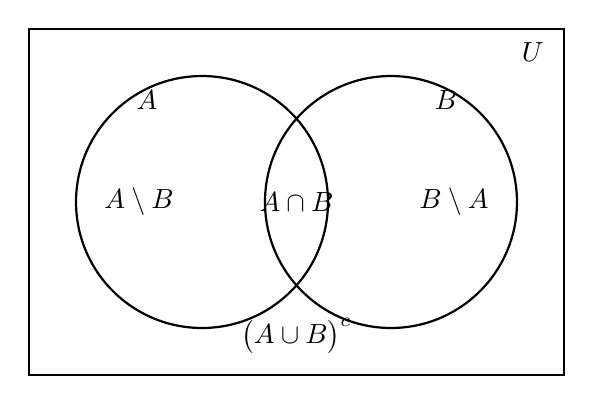
\begin{tikzpicture}[scale=1]
  % Universe
  \draw[thick] (-3.4,-2.2) rectangle (3.4,2.2);
  \node at (3.0,1.9) {$U$};

  % Two sets
  \draw[thick] (-1.2,0) circle (1.6);
  \draw[thick] ( 1.2,0) circle (1.6);

  \node at (-1.9,1.3) {$A$};
  \node at ( 1.9,1.3) {$B$};

  % Label regions (light guidance, no shading needed)
  \node at (0,0) {$A\cap B$};
  \node at (-2.0,0) {$A\setminus B$};
  \node at ( 2.0,0) {$B\setminus A$};
  \node at (0,-1.7) {$\bigl(A\cup B\bigr)^c$};
\end{tikzpicture}
\caption{Regions for $A$, $B$, and their basic combinations inside a universe $U$.}
\end{figure}
\end{example}

\begin{proposition}[Set-builder proof template]\label{prop:setbuilder}
To prove $X=Y$, it suffices to show $X\subseteq Y$ and $Y\subseteq X$, i.e.\ for every $x$,  
$x\in X \Rightarrow x\in Y$ and $x\in Y \Rightarrow x\in X$.
\end{proposition}

\begin{exercise}
Prove the distributive laws:
\[
A\cap (B\cup C) = (A\cap B)\cup (A\cap C),
\qquad
A\cup (B\cap C) = (A\cup B)\cap (A\cup C).
\]
\end{exercise}

\begin{exercise}
Let $A,B\subseteq U$. Prove:
\[
A\setminus B = A\cap B^c,
\qquad
A\triangle B \coloneqq (A\setminus B)\cup (B\setminus A)
\]
satisfies $A\triangle B = (A\cup B)\setminus(A\cap B)$.
\end{exercise}

% -------------------------------------------------
\subsection{Relations, Functions, and Cardinality}

\subsubsection{Relations and Equivalence Relations}

\begin{definition}[Binary relation]
Let $A$ be a set. A \emph{(binary) relation} on $A$ is a subset $R\subseteq A\times A$.  
We write $a\,R\,b$ to mean $(a,b)\in R$.
\end{definition}

\begin{definition}[Equivalence relation]
A relation $\sim$ on $A$ is an \emph{equivalence relation} if it is:
\begin{itemize}
  \item Reflexive: $a\sim a$ for all $a\in A$.
  \item Symmetric: $a\sim b \Rightarrow b\sim a$.
  \item Transitive: $a\sim b$ and $b\sim c \Rightarrow a\sim c$.
\end{itemize}
\end{definition}

\begin{definition}[Equivalence class]
Given $a\in A$, the \emph{equivalence class} of $a$ is
\[
[a] \coloneqq \set*{x\in A \st x\sim a}.
\]
\end{definition}

\begin{theorem}[Equivalence relations and partitions]\label{thm:eq-partition}
If $\sim$ is an equivalence relation on $A$, then the set of equivalence classes
\[
A/{\sim} \coloneqq \set*{[a] \st a\in A}
\]
is a partition of $A$: every element of $A$ lies in exactly one class, and distinct classes are disjoint.

Conversely, every partition of $A$ defines an equivalence relation by declaring $x\sim y$ iff $x$ and $y$ lie in the same part.
\end{theorem}

\begin{proof}
Assume $\sim$ is an equivalence relation.

\emph{Covering:} For any $a\in A$, reflexivity gives $a\sim a$, hence $a\in [a]$. So every $a$ lies in some class.

\emph{Disjointness:} Suppose $[a]\cap [b]\neq \emptyset$. Choose $x\in [a]\cap [b]$. Then $x\sim a$ and $x\sim b$.  
By symmetry, $a\sim x$, and by transitivity, $a\sim b$. Now for any $y\in [a]$, we have $y\sim a\sim b$, so $y\in [b]$. Thus $[a]\subseteq [b]$.  
By symmetry of the argument, $[b]\subseteq [a]$. Hence $[a]=[b]$. So different classes cannot overlap.

Conversely, given a partition $\mathcal{P}$ of $A$, define $x\sim y$ iff $x,y$ are in the same part of $\mathcal{P}$.  
Reflexive/symmetric/transitive follow immediately from the fact that parts are disjoint and cover $A$.
\end{proof}

\begin{example}[Congruence modulo $n$]
Fix $n\in\NN$. Define $a\sim b$ on $\ZZ$ by $a\sim b$ iff $n$ divides $(a-b)$.  
This is an equivalence relation, and its equivalence classes are the residue classes modulo $n$.
\end{example}

\subsubsection{Order Relations and Partially Ordered Sets}

\begin{definition}[Partial order]
A relation $\preceq$ on a set $A$ is a \emph{partial order} if it is:
\begin{itemize}
  \item Reflexive: $a\preceq a$,
  \item Antisymmetric: $a\preceq b$ and $b\preceq a$ imply $a=b$,
  \item Transitive: $a\preceq b$ and $b\preceq c$ imply $a\preceq c$.
\end{itemize}
Then $(A,\preceq)$ is called a \emph{partially ordered set} (poset).
\end{definition}

\begin{example}[Subset order]
For any set $U$, the relation $\subseteq$ is a partial order on $\mathcal{P}(U)$ (the power set of $U$).
\end{example}

\begin{example}[Divisibility order]
On $\NN$, define $a\preceq b$ iff $a$ divides $b$. This is a partial order.
\end{example}

\begin{figure}[H]
\centering
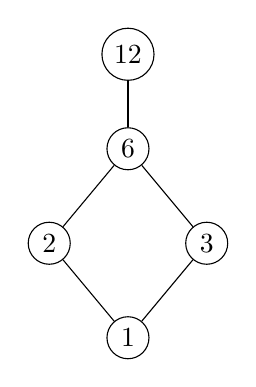
\begin{tikzpicture}[
  node/.style={circle,draw,inner sep=2.5pt},
  scale=1
]
  % Nodes
  \node[node] (1)  at (0,0)    {$1$};
  \node[node] (2)  at (-1,1.2) {$2$};
  \node[node] (3)  at (1,1.2)  {$3$};
  \node[node] (6)  at (0,2.4)  {$6$};
  \node[node] (12) at (0,3.6)  {$12$};

  % Edges (cover relations)
  \draw (1) -- (2);
  \draw (1) -- (3);
  \draw (2) -- (6);
  \draw (3) -- (6);
  \draw (6) -- (12);
\end{tikzpicture}
\caption{A Hasse diagram for divisibility on $\{1,2,3,6,12\}$.}
\end{figure}

\begin{remark}
Later, when we discuss $\sup$ and $\inf$, it is useful to remember that ``being an upper bound'' is an order-theoretic notion: it depends only on the order structure, not on addition/multiplication.
\end{remark}

\subsubsection{Functions: Definitions, Images, Preimages}

\begin{definition}[Function]
A \emph{function} $f$ from a set $A$ to a set $B$ (written $f:A\to B$) assigns to each $a\in A$ a unique element $f(a)\in B$.  
The set $A$ is the \emph{domain}, $B$ the \emph{codomain}, and $f(A)=\set*{f(a)\st a\in A}$ the \emph{image} (or range).
\end{definition}

\begin{definition}[Image and preimage]
Let $f:A\to B$ and let $E\subseteq A$, $S\subseteq B$.
\[
f(E) \coloneqq \set*{f(x)\in B \st x\in E},
\qquad
f^{-1}(S) \coloneqq \set*{x\in A \st f(x)\in S}.
\]
\end{definition}

\begin{proposition}[Basic identities for preimages]\label{prop:preimage}
For any $S,T\subseteq B$,
\[
f^{-1}(S\cup T) = f^{-1}(S)\cup f^{-1}(T),
\qquad
f^{-1}(S\cap T) = f^{-1}(S)\cap f^{-1}(T),
\]
and (complements taken in $B$ and $A$ respectively)
\[
f^{-1}(S^c) = \bigl(f^{-1}(S)\bigr)^c.
\]
\end{proposition}

\begin{proof}
We show the first identity; the others follow similarly by chasing membership.

For $x\in A$,
\begin{align*}
x \in f^{-1}(S\cup T)
&\Longleftrightarrow f(x) \in S\cup T \\
&\Longleftrightarrow \bigl(f(x) \in S \text{ or } f(x) \in T\bigr) \\
&\Longleftrightarrow \bigl(x \in f^{-1}(S) \text{ or } x \in f^{-1}(T)\bigr) \\
&\Longleftrightarrow x \in f^{-1}(S) \cup f^{-1}(T).
\end{align*}
\end{proof}

\begin{proposition}[Image of unions and intersections]\label{prop:image}
For $E_1,E_2\subseteq A$,
\[
f(E_1\cup E_2) = f(E_1)\cup f(E_2),
\qquad
f(E_1\cap E_2) \subseteq f(E_1)\cap f(E_2).
\]
If $f$ is injective (defined below), then equality holds in the intersection statement.
\end{proposition}

\begin{proof}
For unions: $y\in f(E_1\cup E_2)$ iff $y=f(x)$ for some $x\in E_1\cup E_2$, i.e.\ $x\in E_1$ or $x\in E_2$, which is equivalent to $y\in f(E_1)\cup f(E_2)$.

For intersections: if $y\in f(E_1\cap E_2)$ then $y=f(x)$ with $x\in E_1\cap E_2$, hence $y\in f(E_1)$ and $y\in f(E_2)$, so $y\in f(E_1)\cap f(E_2)$. This gives $\subseteq$.  
If $f$ is injective and $y\in f(E_1)\cap f(E_2)$, then $y=f(x_1)=f(x_2)$ with $x_1\in E_1$ and $x_2\in E_2$. Injectivity forces $x_1=x_2\in E_1\cap E_2$, hence $y\in f(E_1\cap E_2)$.
\end{proof}

\subsubsection{Injective, Surjective, Bijective}

\begin{definition}[Injective / surjective / bijective]
Let $f:A\to B$.
\begin{itemize}
  \item $f$ is \emph{injective} (one-to-one) if $f(a_1)=f(a_2)\Rightarrow a_1=a_2$.
  \item $f$ is \emph{surjective} (onto) if $\forall b\in B\ \exists a\in A$ such that $f(a)=b$.
  \item $f$ is \emph{bijective} if it is both injective and surjective.
\end{itemize}
\end{definition}

\begin{figure}[H]
\centering
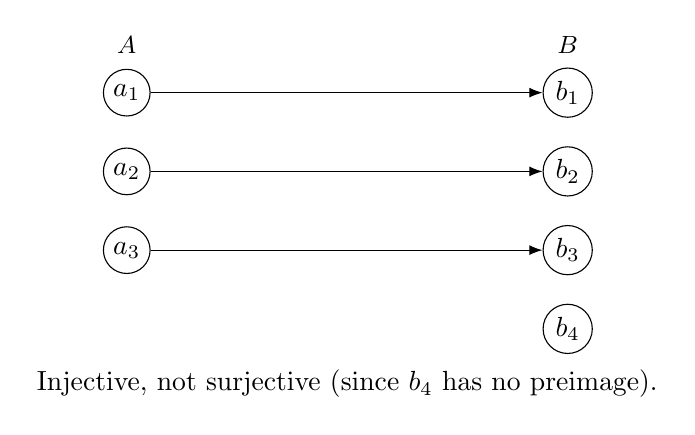
\begin{tikzpicture}[
  >=Latex,
  element/.style={circle,draw,inner sep=2pt},
  label/.style={font=\small}
]
  % Left set A
  \node[label] at (-2.8,1.8) {$A$};
  \node[element] (a1) at (-2.8,1.2) {$a_1$};
  \node[element] (a2) at (-2.8,0.2) {$a_2$};
  \node[element] (a3) at (-2.8,-0.8) {$a_3$};

  % Right set B
  \node[label] at (2.8,1.8) {$B$};
  \node[element] (b1) at (2.8,1.2) {$b_1$};
  \node[element] (b2) at (2.8,0.2) {$b_2$};
  \node[element] (b3) at (2.8,-0.8) {$b_3$};
  \node[element] (b4) at (2.8,-1.8) {$b_4$};

  % Arrows: injective but not surjective (b4 unused)
  \draw[->] (a1) -- (b1);
  \draw[->] (a2) -- (b2);
  \draw[->] (a3) -- (b3);

  \node at (0,-2.5) {Injective, not surjective (since $b_4$ has no preimage).};
\end{tikzpicture}
\caption{A mapping diagram illustrating injectivity and failure of surjectivity.}
\end{figure}

\begin{theorem}[Inverses]\label{thm:inverse}
A function $f:A\to B$ is bijective if and only if there exists a function $g:B\to A$ such that
\[
g\circ f = \id_A
\quad\text{and}\quad
f\circ g = \id_B,
\]
where $\id_A(a)=a$ and $\id_B(b)=b$ are identity maps.
In this case $g$ is unique and is denoted $f^{-1}$.
\end{theorem}

\begin{proof}
If such a $g$ exists, then $f$ is injective: if $f(a_1)=f(a_2)$, applying $g$ gives
\[
a_1 = (g\circ f)(a_1) = (g\circ f)(a_2) = a_2.
\]
Also $f$ is surjective: for any $b\in B$, take $a=g(b)$; then $(f\circ g)(b)=b$ gives $f(a)=b$.

Conversely, if $f$ is bijective, define $g(b)$ to be the unique $a\in A$ such that $f(a)=b$. Then $g$ is well-defined and satisfies the identities.
Uniqueness follows because any $g$ with $g\circ f=\id_A$ must send $b=f(a)$ to $a$.
\end{proof}

\begin{figure}[H]
\centering
\begin{tikzcd}[row sep=large, column sep=huge]
A \arrow[r,"f"] \arrow[dr,"h"'] & B \arrow[d,"g"] \\
& C
\end{tikzcd}
\caption{Composition: $h=g\circ f$. Commutative diagrams help prevent domain/codomain mistakes.}
\end{figure}

\subsubsection{Cardinality: Countable vs.\ Uncountable}

\begin{definition}[Equipotence and cardinality comparison]
Two sets $A$ and $B$ are \emph{equipotent} (same cardinality), written $A\sim B$, if there exists a bijection $f:A\to B$.  
We write $\abs{A}\le \abs{B}$ if there exists an injection $A\to B$.
\end{definition}

\begin{definition}[Countable sets]
A set $A$ is \emph{countable} if it is finite or if there exists a bijection $A\sim \NN$.  
A set that is not countable is called \emph{uncountable}.
\end{definition}

\begin{example}
The sets $\NN$, $\ZZ$, and $\QQ$ are countable; the set $\RR$ is uncountable (proved below).
\end{example}

\begin{theorem}[$\NN\times\NN$ is countable]\label{thm:NxN}
The Cartesian product $\NN\times\NN$ is countable.
\end{theorem}

\begin{proof}
List pairs by increasing sum $m+n$ (a ``diagonal'' enumeration):
\[
(1,1),\ (1,2),(2,1),\ (1,3),(2,2),(3,1),\ \dots
\]
This produces a sequence that hits every pair $(m,n)$ after finitely many steps (namely once the diagonal $m+n$ is reached).  
Thus there is a surjection $\NN\to \NN\times\NN$. Since $\NN\times\NN$ is infinite, one can refine this to a bijection (or equivalently, show $\NN\times\NN$ injects into $\NN$ via the Cantor pairing function in \cref{eq:cantor-pair}).
\end{proof}

\begin{equation}\label{eq:cantor-pair}
\pi(m,n)=\frac{(m+n)(m+n+1)}{2}+n,
\end{equation}
which defines an injection $\pi:\NN_0\times\NN_0\to \NN_0$ (in fact a bijection).

\begin{theorem}[Countable unions of countable sets]\label{thm:countable-union}
If $\{A_n\}_{n\in\NN}$ is a sequence of countable sets, then $\bigcup_{n\in\NN} A_n$ is countable.
\end{theorem}

\begin{proof}
For each $n$, since $A_n$ is countable, there exists a surjection $f_n:\NN\to A_n$.  
Define $F:\NN\times\NN\to \bigcup_{n\in\NN} A_n$ by $F(n,k)=f_n(k)$. This is surjective by construction.  
By \Cref{thm:NxN}, the domain $\NN\times\NN$ is countable, so its image under a surjection is also countable. Hence the union is countable.
\end{proof}

\begin{theorem}[$\QQ$ is countable]\label{thm:Q-countable}
The set of rational numbers $\QQ$ is countable.
\end{theorem}

\begin{proof}
For each $q\in\NN$, define
\[
S_q \coloneqq \set*{\frac{p}{q}\in\QQ \st p\in\ZZ}.
\]
The map $\ZZ\to S_q$ given by $p\mapsto p/q$ is surjective, so each $S_q$ is countable.  
Moreover,
\[
\QQ = \bigcup_{q\in\NN} S_q,
\]
because every rational has some (not necessarily reduced) representation with positive denominator.  
By \Cref{thm:countable-union}, $\QQ$ is countable.
\end{proof}

\begin{remark}[Why duplicates do not matter]
In the union $\bigcup_{q\in\NN} S_q$, the same rational number may appear multiple times (e.g.\ $1/2=2/4$).  
This does not affect countability: a set remains countable even if it is listed with repetitions; removing duplicates only makes the set smaller (and any subset of a countable set is countable).
\end{remark}

\subsubsection{Cantor's Diagonal Argument}

\begin{theorem}[Uncountability of $(0,1)$]\label{thm:cantor}
The interval $(0,1)\subseteq\RR$ is uncountable. Consequently, $\RR$ is uncountable.
\end{theorem}

\begin{proof}
Assume for contradiction that $(0,1)$ is countable. Then we can list its elements as a sequence
\[
x_1,\ x_2,\ x_3,\ \dots
\]
Write each $x_n$ in decimal form:
\[
x_n = 0.a_{n1}a_{n2}a_{n3}\dots,
\]
where each digit $a_{nk}\in\{0,1,2,\dots,9\}$. (If a number has two decimal expansions, choose the one not ending in repeating $9$'s; this can always be done.)

Now define a new number $y\in(0,1)$ by specifying its digits:
\[
y = 0.b_1b_2b_3\dots,
\qquad
b_n \coloneqq
\casesm{
1, & \text{if } a_{nn}\neq 1,\\
2, & \text{if } a_{nn}=1.
}
\]
Then each $b_n\in\{1,2\}$, so $y$ does not end with repeating $9$'s and hence has a unique decimal expansion.

By construction, $y$ differs from $x_n$ in the $n$-th decimal place (since $b_n\neq a_{nn}$). Therefore $y\neq x_n$ for every $n\in\NN$.  
This contradicts the assumption that $\{x_n\}$ lists all elements of $(0,1)$. Hence $(0,1)$ is uncountable.
\end{proof}

\begin{corollary}\label{cor:irrational-uncountable}
The set of irrational numbers $\RR\setminus\QQ$ is uncountable.
\end{corollary}

\begin{proof}
If $\RR\setminus\QQ$ were countable, then $\RR=(\RR\setminus\QQ)\cup\QQ$ would be a union of two countable sets, hence countable by \Cref{thm:countable-union}, contradicting \Cref{thm:cantor}.
\end{proof}

\begin{remark}[Cardinality is preserved under bijection]
A standard technique in analysis is to compare sets by building explicit bijections.
For instance, the map $T:(0,1)\to (a,b)$ given by
\[
T(x)=a+(b-a)x
\]
is a bijection; hence every open interval has the same cardinality as $(0,1)$.

Also, the map $\Phi:(0,1)\to\RR$ defined by
\[
\Phi(x)=\tan\bigl(\pi(x-\tfrac12)\bigr)
\]
is a bijection, showing $(0,1)\sim \RR$. (This is a good example of how functions encode ``same size'' even for infinite sets.)
\end{remark}

\begin{theorem}[Cantor's theorem]\label{thm:cantor-power}
For any set $A$, the power set $\mathcal{P}(A)$ has strictly larger cardinality than $A$:
\[
\abs{A} < \abs{\mathcal{P}(A)}.
\]
\end{theorem}

\begin{proof}
First, there is always an injection $A\to\mathcal{P}(A)$ given by $a\mapsto\{a\}$, so $\abs{A}\le \abs{\mathcal{P}(A)}$.

To show strict inequality, suppose (for contradiction) that there is a surjection $f:A\to \mathcal{P}(A)$.  
Define the set
\[
D \coloneqq \set*{a\in A \st a\notin f(a)}.
\]
Since $f$ is surjective, there exists $d\in A$ with $f(d)=D$. Now ask whether $d\in D$.

\begin{itemize}
  \item If $d\in D$, then by definition of $D$ we must have $d\notin f(d)=D$, contradiction.
  \item If $d\notin D$, then by definition of $D$ we must have $d\in f(d)=D$, contradiction.
\end{itemize}

Both cases contradict, so no surjection $A\to\mathcal{P}(A)$ exists. Hence $\abs{A}<\abs{\mathcal{P}(A)}$.
\end{proof}

\begin{exercise}
Show that the set of all finite subsets of $\NN$ is countable.
\end{exercise}

\begin{exercise}
Let $A$ be countable and $B\subseteq A$. Prove that $B$ is countable.
\end{exercise}

\begin{exercise}
Give an explicit bijection between $\NN$ and $\ZZ$. (Hint: interleave nonnegative and negative integers.)
\end{exercise}

\begin{exercise}
Prove that the set of algebraic numbers is countable. Conclude that there exist transcendental real numbers.
\end{exercise}

\newpage

% =========================
% The Real Number System
% =========================

\section{The Real Number System}

\begin{keyidea}
The real numbers $\RR$ are characterized (up to a unique order-preserving field isomorphism) as the \emph{complete ordered field}.
In practice, we do not rebuild $\RR$ from scratch every time; instead we work from axioms and prove the familiar properties (algebra, inequalities, bounds, and approximation) \emph{rigorously} from those axioms.
\end{keyidea}

% -------------------------------------------------
\subsection{Axiomatic Construction of $\RR$}

\subsubsection{Field Axioms}

\begin{definition}[Field]
A set $F$ equipped with two operations $+$ and $\cdot$ is a \emph{field} if:
\begin{enumerate}[label=(F\arabic*)]
\item \textbf{Addition:} $(F,+)$ is an abelian group. Concretely:
  \begin{enumerate}[label=(\alph*)]
    \item $a+b\in F$ for all $a,b\in F$ (closure).
    \item $(a+b)+c=a+(b+c)$ for all $a,b,c\in F$ (associativity).
    \item $a+b=b+a$ for all $a,b\in F$ (commutativity).
    \item There exists $0\in F$ such that $a+0=a$ for all $a\in F$ (additive identity).
    \item For each $a\in F$, there exists $-a\in F$ such that $a+(-a)=0$ (additive inverse).
  \end{enumerate}
\item \textbf{Multiplication:} $(F\setminus\{0\},\cdot)$ is an abelian group:
  \begin{enumerate}[label=(\alph*)]
    \item $ab\in F$ for all $a,b\in F$ (closure).
    \item $(ab)c=a(bc)$ for all $a,b,c\in F$ (associativity).
    \item $ab=ba$ for all $a,b\in F$ (commutativity).
    \item There exists $1\in F$ with $1\neq 0$ such that $a\cdot 1=a$ for all $a\in F$ (multiplicative identity).
    \item For each $a\in F\setminus\{0\}$, there exists $a^{-1}\in F$ such that $aa^{-1}=1$ (multiplicative inverse).
  \end{enumerate}
\item \textbf{Distributivity:} $a(b+c)=ab+ac$ for all $a,b,c\in F$.
\end{enumerate}
\end{definition}

\begin{remark}
When $F=\RR$, the operations are the usual addition and multiplication. The point of axioms is that every algebraic manipulation must ultimately be justified by these rules (and the consequences derived from them).
\end{remark}

\begin{proposition}[Basic algebraic consequences in a field]\label{prop:field-basic}
Let $F$ be a field and $a,b,c\in F$. Then:
\begin{enumerate}[label=(\alph*)]
\item (\textbf{Additive cancellation}) If $a+c=b+c$, then $a=b$.
\item (\textbf{Multiplicative cancellation}) If $c\neq 0$ and $ac=bc$, then $a=b$.
\item $a\cdot 0 = 0$.
\item (\textbf{Zero-product property}) If $ab=0$, then $a=0$ or $b=0$.
\end{enumerate}
\end{proposition}

\begin{proof}
\begin{enumerate}[label=(\alph*)]
\item Add $(-c)$ to both sides:
\[
a+c=b+c \;\Rightarrow\; (a+c)+(-c)=(b+c)+(-c)
\;\Rightarrow\; a=b.
\]
\item Multiply both sides by $c^{-1}$:
\[
ac=bc \;\Rightarrow\; ac\,c^{-1}=bc\,c^{-1} \;\Rightarrow\; a=b.
\]
\item Using distributivity and additive cancellation:
\[
a\cdot 0 = a(0+0)=a\cdot 0 + a\cdot 0 \;\Rightarrow\; a\cdot 0 = 0.
\]
\item If $ab=0$ and $a\neq 0$, multiply by $a^{-1}$:
\[
ab=0 \;\Rightarrow\; a^{-1}ab=a^{-1}0 \;\Rightarrow\; b=0.
\]
So either $a=0$ or $b=0$.
\end{enumerate}
\end{proof}

\subsubsection{Order Axioms}

\begin{definition}[Ordered field]
A field $F$ is an \emph{ordered field} if it is equipped with a relation $<$ such that:
\begin{enumerate}[label=(O\arabic*)]
\item (\textbf{Trichotomy}) For any $a,b\in F$, exactly one of $a<b$, $a=b$, $a>b$ holds.
\item (\textbf{Transitivity}) If $a<b$ and $b<c$, then $a<c$.
\item (\textbf{Addition preserves order}) If $a<b$, then $a+c<b+c$ for all $c\in F$.
\item (\textbf{Multiplication by positives preserves order}) If $a<b$ and $c>0$, then $ac<bc$.
\end{enumerate}
We also write $a\le b$ to mean $a<b$ or $a=b$.
\end{definition}

\begin{proposition}[Standard inequality rules]\label{prop:ineq-rules}
Let $F$ be an ordered field and $a,b,c,d\in F$.
\begin{enumerate}[label=(\alph*)]
\item If $a<b$ then $-b<-a$.
\item If $0<a$ and $0<b$, then $0<ab$.
\item If $a<b$ and $c<d$, then $a+c<b+d$.
\item If $a<b$ and $0<c$, then $\frac{a}{c}<\frac{b}{c}$.
\item If $a<b$ and $c<0$, then $\frac{a}{c}>\frac{b}{c}$.
\end{enumerate}
\end{proposition}

\begin{proof}
\begin{enumerate}[label=(\alph*)]
\item From $a<b$, add $-a-b$ to both sides:
\[
a + (-a-b) < b + (-a-b) \;\Rightarrow\; -b < -a.
\]
\item Since $0<a$, multiplying the inequality $0<b$ by $a>0$ gives $0\cdot a < ba$, i.e.\ $0<ab$.
\item From $a<b$ add $c$ to get $a+c<b+c$. From $c<d$ add $b$ to get $b+c<b+d$. Combine by transitivity:
\[
a+c < b+c < b+d.
\]
\item If $0<c$, then multiplying $a<b$ by $c^{-1}>0$ preserves the inequality:
\[
a<b \;\Rightarrow\; ac^{-1} < bc^{-1} \;\Rightarrow\; \frac{a}{c}<\frac{b}{c}.
\]
\item If $c<0$, then $-c>0$. By (d),
\[
\frac{a}{-c} < \frac{b}{-c}.
\]
Multiplying by $-1$ reverses order by (a), hence
\[
-\frac{a}{-c} > -\frac{b}{-c} \;\Rightarrow\; \frac{a}{c}>\frac{b}{c}.
\]
\end{enumerate}
\end{proof}

\subsubsection{Absolute Value as an Order-Theoretic Notion}

\begin{definition}[Absolute value]
In an ordered field $F$, define $\abs{x}$ by
\[
\abs{x} \coloneqq
\casesm{
x, & x\ge 0,\\
-x, & x<0.
}
\]
\end{definition}

\begin{proposition}[Basic properties of absolute value]\label{prop:abs-basic}
For all $x,y$ in an ordered field:
\begin{enumerate}[label=(\alph*)]
\item $\abs{x}\ge 0$, and $\abs{x}=0 \iff x=0$.
\item $\abs{xy}=\abs{x}\,\abs{y}$.
\item $\abs{x+y}\le \abs{x}+\abs{y}$ (triangle inequality).
\item $\bigl|\abs{x}-\abs{y}\bigr|\le \abs{x-y}$ (reverse triangle inequality).
\end{enumerate}
\end{proposition}

\begin{proof}
\begin{enumerate}[label=(\alph*)]
\item By definition, $\abs{x}$ equals either $x$ (if $x\ge 0$) or $-x$ (if $x<0$), both of which are $\ge 0$.  
If $\abs{x}=0$, then either $x=0$ or $-x=0$, hence $x=0$. Conversely, if $x=0$ then $\abs{x}=0$.
\item Consider cases based on the signs of $x$ and $y$. For example, if $x\ge 0$ and $y\ge 0$, then $\abs{xy}=xy=\abs{x}\abs{y}$.  
If $x<0$ and $y\ge 0$, then $xy\le 0$ so $\abs{xy}=-(xy)=(-x)y=\abs{x}\abs{y}$, etc. All cases give the same identity.
\item We prove $\abs{x+y}\le \abs{x}+\abs{y}$ by comparing squares (which avoids a long sign split and stays fully rigorous):
since $\abs{t}\ge 0$ and $\abs{t}^2=t^2$, it suffices to show
\[
(x+y)^2 \le \bigl(\abs{x}+\abs{y}\bigr)^2.
\]
Expanding both sides gives
\[
x^2 + 2xy + y^2 \le x^2 + 2\abs{x}\abs{y} + y^2,
\]
which reduces to $xy \le \abs{x}\abs{y}$. This inequality holds because:
\[
-\abs{x}\abs{y} \le xy \le \abs{x}\abs{y},
\]
a consequence of $\abs{x}\abs{y}\ge 0$ and the definition of $\abs{\cdot}$ applied to $xy$. Therefore the triangle inequality follows.
\item Apply the triangle inequality to $x=(x-y)+y$:
\[
\abs{x} = \abs{(x-y)+y} \le \abs{x-y}+\abs{y}
\;\Rightarrow\;
\abs{x}-\abs{y}\le \abs{x-y}.
\]
Swap $x$ and $y$ to also get $\abs{y}-\abs{x}\le \abs{x-y}$. Combining,
\[
-\abs{x-y}\le \abs{x}-\abs{y}\le \abs{x-y},
\]
which is equivalent to $\bigl|\abs{x}-\abs{y}\bigr|\le \abs{x-y}$.
\end{enumerate}
\end{proof}

\subsubsection{Completeness Axiom}

\begin{definition}[Upper bounds and least upper bounds]
Let $S\subseteq \RR$.
\begin{itemize}
\item A number $u\in\RR$ is an \emph{upper bound} of $S$ if $x\le u$ for all $x\in S$.
\item If $S$ has an upper bound, we say $S$ is \emph{bounded above}.
\item A number $s\in\RR$ is the \emph{least upper bound} (or \emph{supremum}) of $S$ if:
  \begin{enumerate}[label=(\roman*)]
    \item $s$ is an upper bound of $S$, and
    \item if $u$ is any upper bound of $S$, then $s\le u$.
  \end{enumerate}
In this case we write $s=\sup S$.
\end{itemize}
\end{definition}

\begin{theorem}[Completeness axiom / Least upper bound property]\label{thm:completeness}
Every nonempty subset $S\subseteq\RR$ that is bounded above has a supremum in $\RR$.
\end{theorem}

\begin{remark}
This axiom is the key feature that distinguishes $\RR$ from $\QQ$. Many deep theorems in analysis (convergence, continuity, compactness) ultimately trace back to completeness.
\end{remark}

\subsubsection{Why $\QQ$ Is Not Complete}

\begin{example}[A bounded set in $\QQ$ with no supremum in $\QQ$]\label{ex:Q-not-complete}
Consider the set
\[
S \coloneqq \set*{q\in\QQ \st q>0 \text{ and } q^2<2}.
\]
\begin{itemize}
\item $S$ is nonempty (e.g.\ $1\in S$) and bounded above in $\QQ$ (e.g.\ $2$ is an upper bound since $q^2<2$ implies $q<2$ for $q>0$).
\item In $\RR$, $\sup S=\sqrt{2}$.
\item But $\sqrt{2}\notin\QQ$, so $\sup S$ does \emph{not} exist in $\QQ$.
\end{itemize}
A more detailed argument shows: if $r\in\QQ$ is an upper bound of $S$, then $r^2>2$; if $r^2>2$ one can construct a smaller rational upper bound, so no least rational upper bound exists.
\end{example}

\begin{remark}
Completeness is not merely about “having more numbers.” It is the precise statement that \emph{bounded monotone approximation processes do not get stuck outside the number system}.
\end{remark}

\begin{exercise}
Let $S\subseteq \RR$ be nonempty and bounded above, and let $s=\sup S$. Prove that $s$ is unique.
\end{exercise}

\newpage

% -------------------------------------------------
\subsection{Bounds and Supremum}

\subsubsection{Upper/Lower Bounds, Max/Min}

\begin{definition}[Lower bound, infimum, boundedness]
Let $S\subseteq\RR$.
\begin{itemize}
\item A number $\ell\in\RR$ is a \emph{lower bound} of $S$ if $\ell\le x$ for all $x\in S$.
\item If $S$ has a lower bound, we say $S$ is \emph{bounded below}.
\item If $S$ is bounded above and below, we say $S$ is \emph{bounded}.
\item The \emph{greatest lower bound} (or \emph{infimum}) is denoted $\inf S$ and defined analogously to $\sup S$.
\end{itemize}
\end{definition}

\begin{definition}[Maximum and minimum]
Let $S\subseteq\RR$.
\begin{itemize}
\item $m\in S$ is a \emph{maximum} of $S$ if $x\le m$ for all $x\in S$. We write $m=\max S$.
\item $n\in S$ is a \emph{minimum} of $S$ if $n\le x$ for all $x\in S$. We write $n=\min S$.
\end{itemize}
\end{definition}

\begin{remark}
A maximum (or minimum) must be an \emph{element} of the set. A supremum (or infimum) need not belong to the set.
For example, $\sup(0,1)=1$ but $(0,1)$ has no maximum.
\end{remark}

\subsubsection{Characterization of the Supremum}

\begin{theorem}[Approximation property of $\sup$]\label{thm:sup-approx}
Let $S\subseteq\RR$ be nonempty and bounded above, and let $s=\sup S$. Then:
\begin{enumerate}[label=(\alph*)]
\item $x\le s$ for all $x\in S$.
\item For every $\eps>0$, there exists $x_\eps\in S$ such that
\[
s-\eps < x_\eps \le s.
\]
Equivalently, $s-\eps$ is \emph{not} an upper bound of $S$ for any $\eps>0$.
\end{enumerate}
Conversely, if $s\in\RR$ satisfies (a) and (b), then $s=\sup S$.
\end{theorem}

\begin{proof}
Assume $s=\sup S$. Part (a) is the definition of upper bound.

For (b), fix $\eps>0$. If no $x\in S$ satisfies $x> s-\eps$, then every $x\in S$ has $x\le s-\eps$, so $s-\eps$ is an upper bound of $S$. This contradicts that $s$ is the \emph{least} upper bound (since then $s\le s-\eps$ would follow). Hence there exists $x_\eps\in S$ with $x_\eps>s-\eps$. Also $x_\eps\le s$ by (a).

Conversely, suppose (a) and (b) hold. Then $s$ is an upper bound. If $u$ is any upper bound with $u<s$, choose $\eps=s-u>0$. By (b), there exists $x_\eps\in S$ with $x_\eps>s-\eps=u$, contradicting that $u$ is an upper bound. Therefore no upper bound is $<s$, so $s$ is the least upper bound.
\end{proof}

\begin{corollary}[When $\sup$ is a maximum]\label{cor:sup-max}
If $S\subseteq\RR$ is nonempty and bounded above, then $\sup S\in S$ if and only if $S$ has a maximum, and in that case $\sup S=\max S$.
\end{corollary}

\begin{proof}
If $\sup S\in S$, then it is an upper bound and belongs to $S$, hence it is a maximum by definition.
Conversely, if $m=\max S$, then $m$ is an upper bound and no smaller number can be an upper bound, so $m=\sup S$.
\end{proof}

\subsubsection{Infimum via Supremum}

\begin{proposition}[Infimum and negation]\label{prop:inf-sup}
If $S\subseteq\RR$ is nonempty and bounded below, then
\[
\inf S = - \sup(-S),
\qquad\text{where } -S\coloneqq \set*{-x \st x\in S}.
\]
\end{proposition}

\begin{proof}
Let $T=-S$. A number $\ell$ is a lower bound of $S$ iff $-\ell$ is an upper bound of $T$.
If $s=\sup T$, then $-s$ is the greatest lower bound of $S$, i.e.\ $\inf S=-s$.
\end{proof}

\subsubsection{Algebra of Supremum and Infimum}

\begin{proposition}[Shifts and scalings]\label{prop:sup-algebra}
Let $S\subseteq\RR$ be nonempty and bounded above, and let $c\in\RR$.
\begin{enumerate}[label=(\alph*)]
\item $\sup(S+c)=\sup S + c$, where $S+c\coloneqq \set*{x+c \st x\in S}$.
\item If $\lambda>0$, then $\sup(\lambda S)=\lambda \sup S$, where $\lambda S\coloneqq \set*{\lambda x \st x\in S}$.
\item If $\lambda<0$, then $\sup(\lambda S)=\lambda \inf S$ (assuming $S$ is bounded below so that $\inf S$ exists).
\end{enumerate}
Analogous statements hold for $\inf$.
\end{proposition}

\begin{proof}
We prove (a) and (b); (c) follows from (b) and \Cref{prop:inf-sup}.

(a) Let $s=\sup S$. For all $x\in S$, we have $x\le s$, so $x+c\le s+c$; hence $s+c$ is an upper bound of $S+c$.
If $u$ is any upper bound of $S+c$, then $u-c$ is an upper bound of $S$, so $s\le u-c$, i.e.\ $s+c\le u$.
Thus $s+c$ is the least upper bound, so $\sup(S+c)=s+c$.

(b) Let $\lambda>0$ and $s=\sup S$. If $x\le s$ for all $x\in S$, then multiplying by $\lambda$ preserves order:
\[
\lambda x \le \lambda s \quad \forall x\in S,
\]
so $\lambda s$ is an upper bound of $\lambda S$.
If $u$ is any upper bound of $\lambda S$, then $u/\lambda$ is an upper bound of $S$ (since $\lambda x\le u \Rightarrow x\le u/\lambda$),
so $s\le u/\lambda$ and hence $\lambda s\le u$.
Therefore $\sup(\lambda S)=\lambda s$.
\end{proof}

\subsubsection{Examples}

\begin{example}
Let $S=(0,1)$. Then $S$ is bounded above and below. One has
\[
\sup S = 1,\qquad \inf S = 0,
\]
but $S$ has neither a maximum nor a minimum.
\end{example}

\begin{example}
Let $S=\set*{1-\frac{1}{n} \st n\in\NN}$. Then $S\subset(0,1)$ and:
\[
\sup S = 1 \quad\text{(not in $S$)},\qquad \inf S = 0 \quad\text{(not in $S$)}.
\]
Moreover, $S$ has a minimum: indeed, $1-\frac{1}{n}$ increases with $n$, so the smallest occurs at $n=1$, giving $\min S=0$?  
Be careful: at $n=1$ we get $1-1=0$, so actually $0\in S$ and $\min S=0$ \emph{does} exist, while $\inf S=0$ as well.
Thus $\min S=\inf S=0$, but $\max S$ does not exist and $\sup S=1$.
\end{example}

\begin{remark}
This example illustrates a common pattern: $\inf S$ can be attained while $\sup S$ is not (or vice versa). The supremum/infimum concepts are designed to handle both situations cleanly.
\end{remark}

\subsubsection{A Key Application: Existence of Square Roots}

\begin{theorem}[Existence and uniqueness of $\sqrt{a}$]\label{thm:sqrt-exists}
For every real number $a>0$, there exists a unique real number $s>0$ such that $s^2=a$.
\end{theorem}

\begin{proof}
\textbf{Uniqueness.} If $s,t>0$ and $s^2=t^2$, then
\[
0 = s^2-t^2 = (s-t)(s+t).
\]
Since $s+t>0$, the zero-product property forces $s-t=0$, hence $s=t$.

\textbf{Existence.} Define
\[
S \coloneqq \set*{x\in\RR \st x\ge 0 \text{ and } x^2 < a}.
\]
Then $S$ is nonempty (since $0\in S$) and bounded above (for instance, if $x\ge a+1$, then $x^2\ge (a+1)^2>a$, so such $x$ cannot lie in $S$; hence $a+1$ is an upper bound).
By completeness, $S$ has a supremum; let $s=\sup S$ with $s\ge 0$.

We claim $s^2=a$. We show $s^2$ cannot be $<a$ nor $>a$.

\medskip
\noindent\emph{Step 1: $s^2\not<a$.}
Assume $s^2<a$. Let
\[
\delta \coloneqq \min\!\left\{1,\ \frac{a-s^2}{2s+2}\right\}.
\]
Note $\delta>0$ because $a-s^2>0$ and $2s+2>0$. Then
\begin{align*}
(s+\delta)^2
&= s^2 + 2s\delta + \delta^2\\
&\le s^2 + 2s\delta + \delta \qquad (\text{since } 0<\delta\le 1 \Rightarrow \delta^2\le \delta)\\
&= s^2 + (2s+1)\delta\\
&\le s^2 + (2s+2)\delta\\
&\le s^2 + (a-s^2) = a.
\end{align*}
So $(s+\delta)^2\le a$, and in particular $(s+\delta)^2<a$ (because equality would force $\delta=0$ by the inequality chain, impossible).
Hence $s+\delta\in S$, contradicting that $s$ is an upper bound of $S$.
Therefore $s^2\not<a$.

\medskip
\noindent\emph{Step 2: $s^2\not>a$.}
Assume $s^2>a$. Choose
\[
\delta \coloneqq \min\!\left\{1,\ \frac{s^2-a}{2s}\right\}.
\]
Here $s>0$ (since $a>0$ and $S$ contains positive numbers; thus $\sup S>0$), so $\delta>0$ is well-defined.
Then
\begin{align*}
(s-\delta)^2
&= s^2 - 2s\delta + \delta^2\\
&\ge s^2 - 2s\delta \qquad (\delta^2\ge 0)\\
&\ge s^2 - (s^2-a)=a.
\end{align*}
Thus $(s-\delta)^2\ge a$, so for every $x\in S$ we must have $x\le s-\delta$; otherwise, if $x> s-\delta$, then $x\ge 0$ and monotonicity of $t\mapsto t^2$ on $[0,\infty)$ gives $x^2>(s-\delta)^2\ge a$, contradicting $x\in S$.
Hence $s-\delta$ is an upper bound of $S$, contradicting the \emph{least} upper bound property of $s$ (since $s-\delta<s$).
Therefore $s^2\not>a$.

Combining Steps 1 and 2, we conclude $s^2=a$. This completes the proof.
\end{proof}

\begin{figure}[H]
\centering
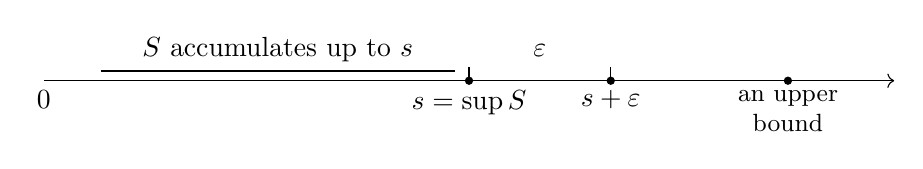
\begin{tikzpicture}[x=9cm,y=1cm]
  % 1. 延长数轴以容纳更宽的间距
  \draw[->] (0,0) -- (1.2,0);
  \node[below] at (0,0) {$0$};

  % 2. 调整坐标位置 (拉大间距解决重叠)
  % 原来是 0.70, 0.84, 0.98 (间距 0.14) -> 改为 0.6, 0.8, 1.05 (间距 >0.2)
  \coordinate (s) at (0.6,0);
  \coordinate (se) at (0.8,0);
  \coordinate (ub) at (1.05,0);

  \fill (s) circle (1.5pt); % 稍微加大一点点点以便看清
  \fill (se) circle (1.5pt);
  \fill (ub) circle (1.5pt);

  % 标签
  \node[below] at (s) {$s=\sup S$};
  \node[below] at (se) {$s+\eps$};
  % 使用 align=center 让长文字换行，或者直接缩短文字
  \node[below, align=center, font=\small] at (ub) {an upper\\bound};

  % Indicate S accumulating from left
  % 调整线条长度以匹配新的 s 位置
  \draw[thick] (0.08,0.12) -- (0.58,0.12);
  \node[above] at (0.33,0.12) {$S$ accumulates up to $s$};

  % 3. 修复报错: 使用相对坐标 ++(0, 0.18)
  % 意思是从当前点 (s) 向上画 0.18 的长度
  \draw (s) -- ++(0,0.18);
  \draw (se) -- ++(0,0.18);
  
  % 标注 epsilon
  % 计算 s 和 se 的中点: (0.6+0.8)/2 = 0.7
  \node[above] at (0.7,0.18) {$\eps$};

\end{tikzpicture}
% 4. 修复 Caption: 补全缺失的 $ 符号
\caption{The supremum $s$ is an upper bound that can be approximated from below by points of $S$.}
\end{figure}

\begin{exercise}
Let $S\subseteq\RR$ be nonempty and bounded above. Show that if $s=\sup S$ and $s\notin S$, then for every $\eps>0$ there exists $x\in S$ with $s-\eps < x < s$.
\end{exercise}

\newpage

% -------------------------------------------------
\subsection{Archimedean Property and Density}

\subsubsection{The Archimedean Principle}

\begin{theorem}[Archimedean property]\label{thm:archimedean}
For every real number $x\in\RR$, there exists $n\in\NN$ such that $n>x$.
Equivalently: for every $y>0$, there exists $n\in\NN$ such that $ny>1$.
\end{theorem}

\begin{proof}
Assume for contradiction that there exists $x\in\RR$ such that $n\le x$ for all $n\in\NN$.
Then $\NN$ is nonempty and bounded above by $x$, so by completeness it has a supremum $s=\sup\NN$.

By \Cref{thm:sup-approx} applied to $S=\NN$, with $\eps=1$, there exists $n_0\in\NN$ such that
\[
s-1 < n_0 \le s.
\]
Add $1$ to obtain $s < n_0+1$. But $n_0+1\in\NN$, contradicting that $s$ is an upper bound of $\NN$.
Therefore no such $x$ exists, and the Archimedean property holds.
\end{proof}

\begin{corollary}\label{cor:small-1n}
For every $\eps>0$, there exists $n\in\NN$ such that $\frac{1}{n}<\eps$.
\end{corollary}

\begin{proof}
Apply \Cref{thm:archimedean} to $x=\frac{1}{\eps}$ to obtain $n>\frac{1}{\eps}$, hence $\frac{1}{n}<\eps$.
\end{proof}

\subsubsection{Integer Part and the Floor Function}

\begin{theorem}[Existence of integer part]\label{thm:floor-exists}
For every $x\in\RR$, there exists a unique integer $m\in\ZZ$ such that
\[
m \le x < m+1.
\]
This integer is denoted $\floor{x}$ (the floor of $x$).
\end{theorem}

\begin{proof}
\textbf{Existence.} Consider the set
\[
A \coloneqq \set*{k\in\ZZ \st k\le x}.
\]
It is nonempty: by the Archimedean property applied to $-x$, there exists $N\in\NN$ with $N>-x$, so $-N<x$, hence $-N\in A$.
Also $A$ is bounded above by $x$ (every element is $\le x$). By completeness, $A$ has a supremum $a=\sup A$.

We claim that $a\in\ZZ$ and $a\le x < a+1$. First, since $a=\sup A$, by \Cref{thm:sup-approx} with $\eps=1$ there exists $k\in A$ such that
\[
a-1 < k \le a.
\]
Because $k\in\ZZ$, the only integers in $(a-1,a]$ are at most one value; in particular, $k$ is the greatest integer $\le a$, hence $k\le a<k+1$.
But $k\le a$ and $a$ is an upper bound of $A$ imply $k$ is actually the largest element of $A$:
if there were $\ell\in A$ with $\ell>k$, then $\ell\ge k+1>a$, contradicting that $a$ is an upper bound.
Thus $k=\max A$ and therefore $a=k\in\ZZ$.

Now $a\in A$ gives $a\le x$. If $x\ge a+1$, then $a+1\le x$ so $a+1\in A$, contradicting maximality of $a$ in $A$.
Hence $x<a+1$.

\textbf{Uniqueness.} If $m\le x<m+1$ and $n\le x<n+1$ with $m,n\in\ZZ$, then $m\le x<n+1$ implies $m<n+1$, hence $m\le n$ (integers).
Similarly $n\le m$. Thus $m=n$.
\end{proof}

\begin{remark}
The floor function provides a precise way to say “choose an integer close to a real number.” It is a standard tool in density proofs and in decimal expansions.
\end{remark}

\subsubsection{Density of $\QQ$ in $\RR$}

\begin{theorem}[Density of rational numbers]\label{thm:Q-dense}
For any real numbers $a<b$, there exists a rational number $q\in\QQ$ such that
\[
a<q<b.
\]
\end{theorem}

\begin{proof}
Let $a<b$. By \Cref{cor:small-1n}, choose $n\in\NN$ such that $\frac{1}{n}<b-a$, i.e.\ $n(b-a)>1$.

Consider the real number $na$. By \Cref{thm:floor-exists}, let $m=\floor{na}\in\ZZ$ so that $m\le na < m+1$.
Define
\[
q \coloneqq \frac{m+1}{n}\in\QQ.
\]
Then $m+1>na$, hence $q>a$. Also
\[
q = \frac{m+1}{n} \le \frac{na+1}{n} = a+\frac{1}{n} < a+(b-a)=b,
\]
because $\frac{1}{n}<b-a$. Therefore $a<q<b$.
\end{proof}

\begin{corollary}\label{cor:many-Q}
Every nonempty open interval contains infinitely many rational numbers.
\end{corollary}

\begin{proof}
Given $a<b$, apply \Cref{thm:Q-dense} to the smaller interval $(a,q)$ to find another rational strictly between, and iterate to get infinitely many distinct rationals.
\end{proof}

\subsubsection{Density of Irrational Numbers}

\begin{theorem}[Density of irrational numbers]\label{thm:irr-dense}
For any real numbers $a<b$, there exists an irrational number $\alpha\in\RR\setminus\QQ$ such that
\[
a<\alpha<b.
\]
\end{theorem}

\begin{proof}
We use $\sqrt{2}\notin\QQ$ (proved earlier in these notes).
Since $a<b$, divide by $\sqrt{2}>0$ to get
\[
\frac{a}{\sqrt{2}} < \frac{b}{\sqrt{2}}.
\]
By \Cref{thm:Q-dense}, choose $q\in\QQ$ such that
\[
\frac{a}{\sqrt{2}} < q < \frac{b}{\sqrt{2}}.
\]
Set $\alpha=q\sqrt{2}$. Then $a<\alpha<b$.
Moreover, if $\alpha$ were rational, then $\sqrt{2}=\alpha/q$ would be rational (since $q\neq 0$), a contradiction. Hence $\alpha$ is irrational.
\end{proof}

\begin{figure}[H]
\centering
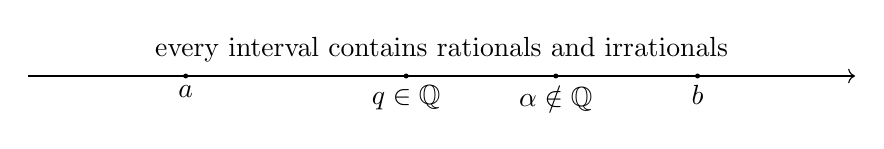
\begin{tikzpicture}[x=10cm,y=1cm]
  \draw[->] (0,0) -- (1.05,0);

  \coordinate (a) at (0.20,0);
  \coordinate (b) at (0.85,0);
  \coordinate (q) at (0.48,0);
  \coordinate (irr) at (0.67,0);

  \fill (a) circle (0.9pt);
  \fill (b) circle (0.9pt);
  \fill (q) circle (0.9pt);
  \fill (irr) circle (0.9pt);

  \node[below] at (a) {$a$};
  \node[below] at (b) {$b$};
  \node[below] at (q) {$q\in\QQ$};
  \node[below] at (irr) {$\alpha\notin\QQ$};

  \draw[thick] (a) -- (b);
  \node[above] at (0.525,0.06) {every interval contains rationals and irrationals};
\end{tikzpicture}
\caption{Both $\QQ$ and $\RR\setminus\QQ$ are dense in $\RR$.}
\end{figure}

\subsubsection{Decimal Expansions}

\begin{theorem}[Decimal expansion for $x\in[0,1)$]\label{thm:decimal-01}
For every $x\in[0,1)$, there exists a sequence of digits $(a_k)_{k\in\NN}$ with $a_k\in\{0,1,\dots,9\}$ such that
\[
x = \sum_{k=1}^{\infty} \frac{a_k}{10^k}.
\]
Moreover, one can choose the digits so that the expansion does not end in repeating $9$'s.
\end{theorem}

\begin{proof}
Define digits recursively. Set $r_0=x$. For $k\ge 1$, define
\[
a_k \coloneqq \floor{10r_{k-1}} \in \{0,1,\dots,9\},
\qquad
r_k \coloneqq 10r_{k-1} - a_k \in [0,1).
\]
(The bounds follow because $a_k \le 10r_{k-1}<a_k+1$ by the floor property.)
Unwinding the recursion gives, for each $n\in\NN$,
\begin{equation}\label{eq:decimal-partial}
x = \sum_{k=1}^{n} \frac{a_k}{10^k} + \frac{r_n}{10^n},
\qquad \text{with } 0\le r_n < 1.
\end{equation}
In particular,
\[
0 \le x - \sum_{k=1}^{n} \frac{a_k}{10^k} = \frac{r_n}{10^n} < \frac{1}{10^n}.
\]
Hence the partial sums converge to $x$, and therefore
\[
x = \lim_{n\to\infty} \sum_{k=1}^{n} \frac{a_k}{10^k}
= \sum_{k=1}^{\infty} \frac{a_k}{10^k}.
\]

If the resulting digits eventually become all $9$, then $x$ has an alternative terminating expansion (see \Cref{prop:999}). We adopt the convention of choosing the non-terminating-$9$ representation to ensure uniqueness.
\end{proof}

\begin{proposition}[Why $0.999\ldots=1$]\label{prop:999}
In $\RR$,
\[
0.999\ldots = 1.
\]
More generally, any terminating decimal has a second representation ending in repeating $9$'s.
\end{proposition}

\begin{proof}
Let $s_n=\sum_{k=1}^{n} 9\cdot 10^{-k}$. Then $s_n=1-10^{-n}$ (a finite geometric sum), so $\lim_{n\to\infty} s_n = 1$.
By definition, $0.999\ldots=\lim_{n\to\infty} s_n$, hence it equals $1$.
\end{proof}

\begin{theorem}[Decimal expansion for general real numbers]\label{thm:decimal-R}
For every real number $x\in\RR$, there exist an integer $m\in\ZZ$ and digits $(a_k)_{k\in\NN}$ such that
\[
x = m + \sum_{k=1}^{\infty} \frac{a_k}{10^k}.
\]
If we require that the digits do not eventually become all $9$, then this representation is unique.
\end{theorem}

\begin{proof}
Let $m=\floor{x}\in\ZZ$ so that $m\le x<m+1$. Then $y=x-m\in[0,1)$.
Apply \Cref{thm:decimal-01} to $y$ to obtain digits $(a_k)$ with
\[
y=\sum_{k=1}^{\infty}\frac{a_k}{10^k}.
\]
Thus $x=m+y$ has the desired form. Uniqueness follows from the uniqueness of $\floor{x}$ and the convention excluding trailing $9$'s.
\end{proof}

\begin{exercise}
Show that if a decimal expansion is eventually periodic (i.e.\ repeats a fixed block of digits from some point onward), then the number is rational.
\end{exercise}

\begin{exercise}
Give an explicit construction of a rational number strictly between $a$ and $b$ without using the floor function, starting from the Archimedean property.
\end{exercise}

\begin{exercise}
Prove that for every $x\in\RR$ and every $n\in\NN$, there exists an integer $m$ such that
\[
\abs{x-\frac{m}{10^n}} \le \frac{1}{10^n}.
\]
Interpret this as “every real can be approximated by decimals with $n$ digits.”
\end{exercise}

\newpage

% =========================
% Sequences and Limits
% =========================

\section{Sequences and Limits}

\begin{keyidea}
A sequence is a function $x:\NN\to\RR$, written $(x_n)_{n\in\NN}$.
The central definition in this chapter is the $\eps$--$N$ definition of convergence.
Once that definition is mastered, most theorems become systematic exercises in quantifiers, inequalities, and completeness.
\end{keyidea}

% -------------------------------------------------
\subsection{Sequences of Real Numbers}

\subsubsection{Definition and Basic Examples}

\begin{definition}[Sequence]
A \emph{sequence of real numbers} is a function $x:\NN\to\RR$.
We write $x(n)=x_n$ and denote the sequence by $(x_n)_{n\in\NN}$, or simply $(x_n)$.
\end{definition}

\begin{example}
\begin{enumerate}[label=(\alph*)]
\item $x_n = \frac{1}{n}$ for $n\in\NN$.
\item $x_n = (-1)^n$ (alternating signs).
\item $x_n = \sqrt{n}$ (unbounded, diverges to $+\infty$).
\item $x_n = \left(1+\frac{1}{n}\right)^n$ (approaches $e$, later proved carefully).
\end{enumerate}
\end{example}

\begin{definition}[Bounded sequence]
A sequence $(x_n)$ is \emph{bounded} if there exists $M>0$ such that $\abs{x_n}\le M$ for all $n\in\NN$.
Equivalently, the set $\{x_n:n\in\NN\}$ is a bounded subset of $\RR$.
\end{definition}

\subsubsection{Convergence and Divergence}

\begin{definition}[Limit of a sequence]\label{def:seq-limit}
Let $(x_n)$ be a sequence and let $L\in\RR$.
We say $x_n$ \emph{converges to} $L$, and write $x_n\to L$ or $\lim_{n\to\infty}x_n=L$, if
\[
\forall \eps>0\ \exists N\in\NN\ \forall n\in\NN,\quad n\ge N \Rightarrow \abs{x_n-L}<\eps.
\]
If no such $L$ exists, we say $(x_n)$ \emph{diverges}.
\end{definition}

\begin{remark}[How to read the definition]
The definition says: \emph{no matter how small} a tolerance $\eps$ you demand, \emph{eventually} all terms of the sequence lie within the interval $(L-\eps,\,L+\eps)$.
The index $N$ may depend on $\eps$.
\end{remark}

\begin{definition}[Divergence phrased with quantifiers]
A sequence $(x_n)$ does \emph{not} converge to $L$ if and only if
\[
\exists \eps_0>0\ \forall N\in\NN\ \exists n\in\NN,\quad n\ge N \ \text{and}\  \abs{x_n-L}\ge \eps_0.
\]
This is exactly the logical negation of \Cref{def:seq-limit}.
\end{definition}

\begin{example}[$\frac1n\to 0$]\label{ex:1n-to-0}
Let $x_n=\frac{1}{n}$. We prove $x_n\to 0$.
Given $\eps>0$, by the Archimedean property (proved in the previous chapter), choose $N\in\NN$ such that $N>\frac{1}{\eps}$.
Then for all $n\ge N$,
\[
\abs{x_n-0}=\frac{1}{n}\le \frac{1}{N}<\eps.
\]
Hence $\lim_{n\to\infty}\frac{1}{n}=0$.
\end{example}

\begin{example}[A divergent bounded sequence]
Let $x_n=(-1)^n$. Suppose $x_n\to L$. Taking $\eps=\tfrac12$, there exists $N$ such that $n\ge N$ implies $\abs{x_n-L}<\tfrac12$.
But both $1$ and $-1$ occur infinitely often among the terms, so for $n\ge N$ we must have simultaneously
\[
\abs{1-L}<\tfrac12\quad \text{and}\quad \abs{-1-L}<\tfrac12,
\]
which is impossible because those inequalities imply $L\in(1/2,3/2)$ and $L\in(-3/2,-1/2)$ at the same time.
Therefore $( (-1)^n )$ diverges.
\end{example}

\begin{figure}[H]
\centering
\begin{tikzpicture}[x=9cm,y=3cm]
  % axes
  \draw[->] (0,0) -- (1.05,0) node[right] {$n$};
  \draw[->] (0,0) -- (0,1.05) node[above] {$x_n$};

  % reference levels
  \draw[densely dashed] (0,0.25) -- (1.02,0.25) node[right] {$0$};
  \draw[densely dashed] (0,0.75) -- (1.02,0.75) node[right] {$1$};

  % points for 1/n approaching 0 (scaled: x = n/16, y ~ 0.25 + 0.5*(1/n))
  \foreach \n/\xx in {1/0.10,2/0.18,3/0.25,4/0.31,5/0.36,6/0.40,8/0.48,10/0.56,12/0.63,16/0.80} {
    \fill (\xx,{0.25+0.5*(1/\n)}) circle (1.2pt);
  }
  \node at (0.78,0.44) {$x_n=\frac1n$};

  % points for (-1)^n (scaled to 0.25 and 0.75)
  \foreach \k/\xx in {1/0.10,2/0.18,3/0.25,4/0.31,5/0.36,6/0.40,7/0.44,8/0.48,9/0.52,10/0.56} {
    \pgfmathparse{mod(\k,2)==0 ? 0.75 : 0.05}
    \fill (\xx,\pgfmathresult) circle (1.2pt);
  }
  \node at (0.72,0.12) {$x_n=(-1)^n$};
\end{tikzpicture}
\caption{A convergent sequence $\frac{1}{n}\to 0$ versus a bounded divergent sequence $(-1)^n$.}
\end{figure}

\subsubsection{Uniqueness of Limits}

\begin{theorem}[Uniqueness of limits]\label{thm:unique-limit}
If a sequence $(x_n)$ converges, then its limit is unique.
That is, if $x_n\to L$ and $x_n\to M$, then $L=M$.
\end{theorem}

\begin{proof}
Assume $x_n\to L$ and $x_n\to M$. Let $\eps>0$.
Choose $N_1$ such that $n\ge N_1\Rightarrow \abs{x_n-L}<\eps/2$, and choose $N_2$ such that $n\ge N_2\Rightarrow \abs{x_n-M}<\eps/2$.
For $n\ge N=\max\{N_1,N_2\}$, the triangle inequality gives
\[
\abs{L-M}\le \abs{L-x_n}+\abs{x_n-M}<\frac{\eps}{2}+\frac{\eps}{2}=\eps.
\]
Since $\eps>0$ is arbitrary, we must have $\abs{L-M}=0$, hence $L=M$.
\end{proof}

\subsubsection{Convergent Sequences Are Bounded}

\begin{proposition}\label{prop:conv-bdd}
If $x_n\to L$, then $(x_n)$ is bounded.
\end{proposition}

\begin{proof}
Take $\eps=1$. Then there exists $N$ such that $n\ge N \Rightarrow \abs{x_n-L}<1$, hence $\abs{x_n}\le \abs{L}+1$ for $n\ge N$.
Let
\[
M \coloneqq \max\Bigl\{\abs{x_1},\dots,\abs{x_{N-1}},\,\abs{L}+1\Bigr\}.
\]
Then $\abs{x_n}\le M$ for all $n\in\NN$.
\end{proof}

\subsubsection{Limit Laws}

\begin{theorem}[Algebraic limit laws]\label{thm:limit-laws}
Let $(x_n)$ and $(y_n)$ be sequences with $x_n\to x$ and $y_n\to y$.
Then:
\begin{enumerate}[label=(\alph*)]
\item $x_n+y_n\to x+y$.
\item $x_ny_n\to xy$.
\item For any $c\in\RR$, $cx_n\to cx$.
\item If $y\neq 0$ and $y_n\neq 0$ for all sufficiently large $n$, then $\frac{x_n}{y_n}\to \frac{x}{y}$.
\end{enumerate}
\end{theorem}

\begin{proof}
\begin{enumerate}[label=(\alph*)]
\item Given $\eps>0$, choose $N_1$ so that $\abs{x_n-x}<\eps/2$ for $n\ge N_1$, and $N_2$ so that $\abs{y_n-y}<\eps/2$ for $n\ge N_2$.
Then for $n\ge N=\max\{N_1,N_2\}$,
\[
\abs{(x_n+y_n)-(x+y)}\le \abs{x_n-x}+\abs{y_n-y}<\eps.
\]

\item First note that $y_n\to y$ implies $(y_n)$ is bounded by \Cref{prop:conv-bdd}; similarly $(x_n)$ is bounded.
Let $M>0$ be such that $\abs{x_n}\le M$ and $\abs{y_n}\le M$ for all $n$.
Then
\[
x_ny_n-xy = x_n(y_n-y) + y(x_n-x),
\]
so by the triangle inequality
\[
\abs{x_ny_n-xy}\le \abs{x_n}\,\abs{y_n-y} + \abs{y}\,\abs{x_n-x}
\le M\abs{y_n-y} + \abs{y}\abs{x_n-x}.
\]
Given $\eps>0$, choose $N_1$ such that $\abs{y_n-y}<\eps/(2M)$ for $n\ge N_1$, and choose $N_2$ such that $\abs{x_n-x}<\eps/(2(\abs{y}+1))$ for $n\ge N_2$.
Then for $n\ge N=\max\{N_1,N_2\}$,
\[
\abs{x_ny_n-xy} < \frac{\eps}{2} + \frac{\abs{y}}{\abs{y}+1}\cdot\frac{\eps}{2} \le \eps.
\]

\item This is immediate from $\abs{cx_n-cx}=\abs{c}\,\abs{x_n-x}$.

\item Since $y_n\to y\neq 0$, take $\eps_0=\abs{y}/2>0$. Then there exists $N_0$ such that $n\ge N_0\Rightarrow \abs{y_n-y}<\abs{y}/2$.
Hence for $n\ge N_0$,
\[
\abs{y_n}\ge \abs{y}-\abs{y_n-y}>\abs{y}-\frac{\abs{y}}{2}=\frac{\abs{y}}{2},
\]
so $y_n\neq 0$ for $n\ge N_0$ and the reciprocals are well-defined.

Now write
\[
\frac{x_n}{y_n}-\frac{x}{y}=\frac{xy_n-x_ny}{yy_n}=\frac{x(y_n-y)+y(x-x_n)}{yy_n}.
\]
Taking absolute values and using the lower bound on $\abs{y_n}$ for large $n$,
\[
\abs{\frac{x_n}{y_n}-\frac{x}{y}}
\le \frac{\abs{x}\,\abs{y_n-y}+\abs{y}\,\abs{x_n-x}}{\abs{y}\,\abs{y_n}}
\le \frac{2}{\abs{y}^2}\bigl(\abs{x}\,\abs{y_n-y}+\abs{y}\,\abs{x_n-x}\bigr)
\]
for all $n\ge N_0$.
Choose $N_1$ so that $\abs{y_n-y}<\frac{\eps\abs{y}^2}{4(\abs{x}+1)}$ for $n\ge N_1$ and $N_2$ so that $\abs{x_n-x}<\frac{\eps\abs{y}}{4}$ for $n\ge N_2$.
Then for $n\ge \max\{N_0,N_1,N_2\}$, the right-hand side is $<\eps$.
\end{enumerate}
\end{proof}

\subsubsection{Order Properties and the Squeeze Theorem}

\begin{proposition}[Limit preserves inequalities]\label{prop:limit-order}
If $x_n\to x$ and $y_n\to y$, and if $x_n\le y_n$ for all $n$, then $x\le y$.
\end{proposition}

\begin{proof}
Assume for contradiction that $x>y$. Let $\eps=\frac{x-y}{3}>0$.
Choose $N_1$ such that $n\ge N_1\Rightarrow \abs{x_n-x}<\eps$, and $N_2$ such that $n\ge N_2\Rightarrow \abs{y_n-y}<\eps$.
For $n\ge N=\max\{N_1,N_2\}$,
\[
x_n > x-\eps = \frac{2x+y}{3}
\quad\text{and}\quad
y_n < y+\eps = \frac{x+2y}{3}.
\]
Since $\frac{2x+y}{3}>\frac{x+2y}{3}$ (because $x>y$), we get $x_n>y_n$ for all $n\ge N$, contradicting $x_n\le y_n$.
Thus $x\le y$.
\end{proof}

\begin{theorem}[Squeeze theorem]\label{thm:squeeze}
Suppose $a_n\le x_n\le b_n$ for all sufficiently large $n$.
If $a_n\to L$ and $b_n\to L$, then $x_n\to L$.
\end{theorem}

\begin{proof}
Let $\eps>0$. Choose $N_1$ such that $n\ge N_1\Rightarrow \abs{a_n-L}<\eps$, hence $L-\eps<a_n$.
Choose $N_2$ such that $n\ge N_2\Rightarrow \abs{b_n-L}<\eps$, hence $b_n<L+\eps$.
Also choose $N_0$ such that $n\ge N_0\Rightarrow a_n\le x_n\le b_n$.
For $n\ge N=\max\{N_0,N_1,N_2\}$,
\[
L-\eps<a_n\le x_n\le b_n<L+\eps,
\]
so $\abs{x_n-L}<\eps$. Hence $x_n\to L$.
\end{proof}

\begin{example}[$\frac{\sin n}{n}\to 0$]\label{ex:sin-n-over-n}
Since $\abs{\sin n}\le 1$ for all $n$, we have
\[
-\frac{1}{n}\le \frac{\sin n}{n}\le \frac{1}{n}.
\]
By \Cref{ex:1n-to-0}, both bounds converge to $0$, hence by \Cref{thm:squeeze} we conclude $\frac{\sin n}{n}\to 0$.
\end{example}

\begin{exercise}
Prove that if $x_n\to 0$ and $(y_n)$ is bounded, then $x_ny_n\to 0$.
\end{exercise}

\begin{exercise}
Let $x_n\to L$. Show that $\abs{x_n}\to \abs{L}$.
(Hint: use the reverse triangle inequality.)
\end{exercise}

\newpage

% -------------------------------------------------
\subsection{Monotone and Bounded Sequences}

\subsubsection{Monotonicity}

\begin{definition}[Monotone sequences]
A sequence $(x_n)$ is
\begin{itemize}
\item \emph{increasing} if $x_{n+1}\ge x_n$ for all $n$;
\item \emph{strictly increasing} if $x_{n+1}>x_n$ for all $n$;
\item \emph{decreasing} if $x_{n+1}\le x_n$ for all $n$;
\item \emph{monotone} if it is increasing or decreasing.
\end{itemize}
\end{definition}

\begin{example}
The sequence $x_n=1-\frac{1}{n}$ is increasing and bounded above by $1$.
The sequence $y_n=\frac{1}{n}$ is decreasing and bounded below by $0$.
\end{example}

\subsubsection{Monotone Convergence Theorem}

\begin{theorem}[Monotone Convergence Theorem]\label{thm:monotone-convergence}
\begin{enumerate}[label=(\alph*)]
\item If $(x_n)$ is increasing and bounded above, then $(x_n)$ converges and
\[
\lim_{n\to\infty} x_n = \sup\{x_n:n\in\NN\}.
\]
\item If $(x_n)$ is decreasing and bounded below, then $(x_n)$ converges and
\[
\lim_{n\to\infty} x_n = \inf\{x_n:n\in\NN\}.
\]
\end{enumerate}
\end{theorem}

\begin{proof}
We prove (a); (b) is analogous.

Let $S=\{x_n:n\in\NN\}$. Since $(x_n)$ is bounded above, $S$ is bounded above; since the sequence exists, $S$ is nonempty.
By completeness, let $s=\sup S$.

We claim $x_n\to s$. Let $\eps>0$.
By the approximation property of the supremum, there exists some index $N$ such that
\[
s-\eps < x_N \le s.
\]
Since $(x_n)$ is increasing, for every $n\ge N$ we have $x_n\ge x_N> s-\eps$.
Also $x_n\le s$ for all $n$ because $s$ is an upper bound.
Thus for $n\ge N$,
\[
s-\eps < x_n \le s \quad \Rightarrow\quad \abs{x_n-s}<\eps.
\]
Therefore $x_n\to s$.
\end{proof}

\begin{figure}[H]
\centering
\begin{tikzpicture}[x=10cm,y=2.2cm]
  % number line
  \draw[->] (0,0) -- (1.05,0);
  \coordinate (s) at (0.86,0);
  \fill (s) circle (1.1pt);
  \node[below] at (s) {$s=\sup S$};

  % increasing dots approaching s
  \foreach \xx/\lab in {0.18/{x_1},0.32/{x_2},0.44/{x_3},0.54/{x_4},0.62/{x_5},0.69/{x_6},0.74/{x_7},0.78/{x_8},0.81/{x_9}}{
    \fill (\xx,0) circle (1.1pt);
  }

  % --- 修复重叠部分 ---
  
  % 1. 拉长虚线：从 0.18 延伸到 0.45，为文字腾出空间
  \draw[densely dashed] (0.76,0.45) -- (0.76,-0.18);
  \draw[densely dashed] (0.96,0.45) -- (0.96,-0.18);
  
  % 2. 顶层标签：将 s +/- eps 移到最上方 (y=0.45)
  \node[above] at (0.86,0.45) {$s\pm\eps$};

  % 3. 中间层：绘制横线和说明文字 (y=0.25)
  % 稍微缩小字体 (\footnotesize) 以防横向挤压
  \draw[thick] (0.76,0.25) -- (0.96,0.25);
  \node[above, font=\footnotesize] at (0.86,0.25) {eventually inside};

\end{tikzpicture}
\caption{An increasing bounded sequence converges to $\sup S$.}
\end{figure}

\subsubsection{Nested Interval Lemma (Useful Tool)}

\begin{theorem}[Nested Interval Property]\label{thm:nested-interval}
Let $(I_n)$ be a sequence of closed intervals
\[
I_n=[a_n,b_n]\subseteq \RR
\]
such that $I_{n+1}\subseteq I_n$ for all $n$ (nested), and $a_n\le b_n$.
Then
\[
\bigcap_{n=1}^{\infty} I_n \neq \emptyset.
\]
If moreover $b_n-a_n\to 0$, then the intersection consists of exactly one point.
\end{theorem}

\begin{proof}
Since the intervals are nested, $(a_n)$ is increasing and bounded above by $b_1$, while $(b_n)$ is decreasing and bounded below by $a_1$.
Let
\[
a=\sup\{a_n:n\in\NN\}, \qquad b=\inf\{b_n:n\in\NN\}.
\]
For each $n$, we have $a_n\le a$ (as $a$ is an upper bound of $\{a_n\}$) and $b\le b_n$ (as $b$ is a lower bound of $\{b_n\}$).
Also $a_n\le b_n$ implies $a\le b$ (one way: take limits using \Cref{prop:limit-order} after applying \Cref{thm:monotone-convergence} to $(a_n)$ and $(b_n)$).
Hence $a\in [a_n,b_n]=I_n$ for all $n$ (because $a_n\le a\le b_n$), so $a\in \bigcap_{n=1}^\infty I_n$ and the intersection is nonempty.

If additionally $b_n-a_n\to 0$, and $x,y$ are in the intersection, then for every $n$ we have $x,y\in [a_n,b_n]$, so $\abs{x-y}\le b_n-a_n$.
Letting $n\to\infty$ yields $\abs{x-y}=0$, hence $x=y$.
\end{proof}

\subsubsection{Bolzano--Weierstrass Theorem}

\begin{theorem}[Bolzano--Weierstrass]\label{thm:bolzano-weierstrass}
Every bounded sequence in $\RR$ has a convergent subsequence.
\end{theorem}

\begin{proof}
Let $(x_n)$ be bounded. Then there exists an interval $I_1=[\alpha,\beta]$ such that $x_n\in I_1$ for all $n$ (e.g.\ take $\alpha=-M$, $\beta=M$ where $\abs{x_n}\le M$).

Bisect $I_1$ into two closed intervals of equal length:
\[
I_1^{(L)}=\left[\alpha,\frac{\alpha+\beta}{2}\right],
\qquad
I_1^{(R)}=\left[\frac{\alpha+\beta}{2},\beta\right].
\]
At least one of these contains infinitely many terms of the sequence (otherwise the union would contain only finitely many terms).
Choose $I_2$ to be a half-interval containing infinitely many terms, and then choose an index $n_1$ such that $x_{n_1}\in I_2$.

Now repeat: bisect $I_2$ into two halves, choose $I_3\subseteq I_2$ that contains infinitely many terms, and pick $n_2>n_1$ such that $x_{n_2}\in I_3$.
Proceed inductively. We obtain:
\begin{itemize}
\item a nested sequence of closed intervals $I_k=[a_k,b_k]$ with $I_{k+1}\subseteq I_k$,
\item lengths $b_k-a_k=\frac{\beta-\alpha}{2^{k-1}}\to 0$,
\item indices $n_1<n_2<\cdots$ such that $x_{n_k}\in I_{k+1}$ for each $k$.
\end{itemize}

By \Cref{thm:nested-interval}, the intersection $\bigcap_{k=1}^{\infty} I_k$ contains exactly one point; call it $L$.
We claim $x_{n_k}\to L$. Let $\eps>0$.
Choose $K$ such that $b_K-a_K<\eps$ (possible since $b_k-a_k\to 0$).
For $k\ge K$, we have $x_{n_k}\in I_{k+1}\subseteq I_K=[a_K,b_K]$ and also $L\in I_K$.
Hence
\[
\abs{x_{n_k}-L}\le b_K-a_K<\eps.
\]
Therefore the subsequence $(x_{n_k})$ converges to $L$.
\end{proof}

\begin{remark}
Bolzano--Weierstrass is a compactness statement in disguise: in $\RR$, boundedness is enough to guarantee subsequential convergence.
Later, this will be formalized as ``closed and bounded sets are compact'' (Heine--Borel).
\end{remark}

\subsubsection{Cauchy Sequences (Optional but Fundamental)}

\begin{definition}[Cauchy sequence]\label{def:cauchy}
A sequence $(x_n)$ is \emph{Cauchy} if
\[
\forall \eps>0\ \exists N\in\NN\ \forall m,n\in\NN,\quad m,n\ge N \Rightarrow \abs{x_n-x_m}<\eps.
\]
\end{definition}

\begin{proposition}\label{prop:conv-implies-cauchy}
Every convergent sequence is Cauchy.
\end{proposition}

\begin{proof}
Assume $x_n\to L$. Let $\eps>0$ and choose $N$ such that $n\ge N\Rightarrow \abs{x_n-L}<\eps/2$.
Then for $m,n\ge N$,
\[
\abs{x_n-x_m}\le \abs{x_n-L}+\abs{L-x_m}<\frac{\eps}{2}+\frac{\eps}{2}=\eps.
\]
\end{proof}

\begin{theorem}[Cauchy completeness of $\RR$]\label{thm:cauchy-complete}
Every Cauchy sequence in $\RR$ converges.
\end{theorem}

\begin{proof}
Let $(x_n)$ be Cauchy. First, $(x_n)$ is bounded: take $\eps=1$ and choose $N$ so that $m,n\ge N\Rightarrow \abs{x_n-x_m}<1$.
Fix $m=N$. Then for $n\ge N$, $\abs{x_n}\le \abs{x_N}+1$; together with finitely many initial terms, this gives boundedness.

By \Cref{thm:bolzano-weierstrass}, $(x_n)$ has a convergent subsequence $x_{n_k}\to L$.
We show the full sequence converges to $L$.

Let $\eps>0$. Since $(x_n)$ is Cauchy, choose $N_1$ such that $m,n\ge N_1\Rightarrow \abs{x_n-x_m}<\eps/2$.
Since $x_{n_k}\to L$, choose $K$ such that $k\ge K\Rightarrow \abs{x_{n_k}-L}<\eps/2$.
Also choose $k\ge K$ with $n_k\ge N_1$ (possible because $n_k\to\infty$).
Then for any $n\ge N_1$,
\[
\abs{x_n-L}\le \abs{x_n-x_{n_k}}+\abs{x_{n_k}-L}<\frac{\eps}{2}+\frac{\eps}{2}=\eps.
\]
Thus $x_n\to L$.
\end{proof}

\begin{exercise}
Show that a sequence is Cauchy if and only if it is bounded and has the property that every subsequence has a further subsequence converging to the same limit.
\end{exercise}

\newpage

% -------------------------------------------------
\subsection{Subsequences and Limit Points}

\subsubsection{Subsequences}

\begin{definition}[Subsequence]
Let $(x_n)$ be a sequence. A \emph{subsequence} is a sequence of the form $(x_{n_k})_{k\in\NN}$ where
\[
n_1<n_2<n_3<\cdots
\]
is a strictly increasing sequence of indices in $\NN$.
\end{definition}

\begin{remark}
A subsequence is obtained by \emph{deleting terms without changing the order of the remaining ones}.
The map $k\mapsto n_k$ must be strictly increasing; otherwise you could repeat indices, which would destroy key theorems.
\end{remark}

\begin{proposition}\label{prop:subsequence-limit}
If $x_n\to L$, then every subsequence $x_{n_k}$ also converges to $L$.
\end{proposition}

\begin{proof}
Let $\eps>0$. Choose $N$ such that $n\ge N\Rightarrow \abs{x_n-L}<\eps$.
Since $n_k\to\infty$ and is increasing, there exists $K$ such that $k\ge K\Rightarrow n_k\ge N$.
Then for $k\ge K$, $\abs{x_{n_k}-L}<\eps$. Hence $x_{n_k}\to L$.
\end{proof}

\subsubsection{Limit Points (Cluster Points)}

\begin{definition}[Limit point of a sequence]\label{def:limit-point}
A number $\ell\in\RR$ is called a \emph{limit point} (or \emph{cluster point}) of $(x_n)$ if there exists a subsequence $(x_{n_k})$ such that $x_{n_k}\to \ell$.
\end{definition}

\begin{example}
For $x_n=(-1)^n$, the limit points are $1$ and $-1$ (take the even and odd subsequences).
For $x_n=\frac{1}{n}$, the only limit point is $0$.
\end{example}

\begin{proposition}[Characterization via infinitely many terms]\label{prop:limit-point-char}
A number $\ell\in\RR$ is a limit point of $(x_n)$ if and only if
\[
\forall \eps>0,\ \text{the set } \{n\in\NN:\abs{x_n-\ell}<\eps\}\ \text{is infinite}.
\]
\end{proposition}

\begin{proof}
($\Rightarrow$) If $\ell$ is a limit point, there exists a subsequence $x_{n_k}\to \ell$.
Fix $\eps>0$. Then there exists $K$ such that $k\ge K\Rightarrow \abs{x_{n_k}-\ell}<\eps$.
Thus infinitely many indices (namely $n_K,n_{K+1},\dots$) satisfy $\abs{x_n-\ell}<\eps$.

($\Leftarrow$) Assume the stated infinitude property. Construct a subsequence recursively:
choose $n_1$ with $\abs{x_{n_1}-\ell}<1$ (possible since infinitely many exist),
then choose $n_2>n_1$ with $\abs{x_{n_2}-\ell}<1/2$, etc.
In general, after choosing $n_k$, choose $n_{k+1}>n_k$ with $\abs{x_{n_{k+1}}-\ell}<1/(k+1)$.
This is possible because the set of indices with $\abs{x_n-\ell}<1/(k+1)$ is infinite, hence contains indices larger than $n_k$.
Then $\abs{x_{n_k}-\ell}<1/k\to 0$, so $x_{n_k}\to \ell$.
\end{proof}

\subsubsection{$\limsup$ and $\liminf$}

\begin{definition}[Tail suprema and tail infima]\label{def:tail-sup-inf}
For a sequence $(x_n)$ define, for each $n\in\NN$,
\[
s_n \coloneqq \sup\{x_k:k\ge n\},
\qquad
i_n \coloneqq \inf\{x_k:k\ge n\}.
\]
(These are well-defined in $\RR$ whenever the sequence is bounded above/below respectively; in particular for bounded sequences both exist.)
\end{definition}

\begin{proposition}\label{prop:tail-monotone}
If $(x_n)$ is bounded, then $(s_n)$ is decreasing and $(i_n)$ is increasing.
Moreover, for every $n$,
\[
i_n \le x_n \le s_n
\quad\text{and}\quad
i_n \le s_n.
\]
\end{proposition}

\begin{proof}
As $n$ increases, the tail set $\{x_k:k\ge n\}$ becomes smaller (fewer elements).
Taking $\sup$ over a smaller set cannot increase: hence $s_{n+1}\le s_n$, so $(s_n)$ is decreasing.
Similarly, taking $\inf$ over a smaller set cannot decrease: hence $i_{n+1}\ge i_n$, so $(i_n)$ is increasing.
Finally, $x_n$ is an element of the tail set at index $n$, hence it lies between the tail infimum and supremum.
\end{proof}

\begin{definition}[Limit superior and limit inferior]\label{def:limsup-liminf}
For a bounded sequence $(x_n)$, define
\[
\limsup_{n\to\infty} x_n \coloneqq \lim_{n\to\infty} s_n,
\qquad
\liminf_{n\to\infty} x_n \coloneqq \lim_{n\to\infty} i_n,
\]
where the limits exist by the Monotone Convergence Theorem because $(s_n)$ is decreasing and bounded below, and $(i_n)$ is increasing and bounded above.
\end{definition}

\begin{remark}
Even when $(x_n)$ is not convergent, the tails still have a well-defined ``eventual ceiling'' $s_n$ and ``eventual floor'' $i_n$.
The quantities $\limsup x_n$ and $\liminf x_n$ capture the long-term upper and lower accumulation behavior of the sequence.
\end{remark}

\begin{theorem}[Basic properties of $\limsup$ and $\liminf$]\label{thm:limsup-liminf-basic}
Let $(x_n)$ be bounded and define $L^+=\limsup x_n$ and $L^-=\liminf x_n$.
Then:
\begin{enumerate}[label=(\alph*)]
\item $L^- \le L^+$.
\item $L^+$ and $L^-$ are limit points of $(x_n)$.
\item A number $\ell$ is a limit point of $(x_n)$ if and only if $L^-\le \ell \le L^+$ \emph{and} for every $\eps>0$ there are infinitely many $n$ with $\abs{x_n-\ell}<\eps$.
(In particular, all limit points lie in $[L^-,L^+]$.)
\item The sequence $(x_n)$ converges to $L$ if and only if $\limsup x_n=\liminf x_n=L$.
\end{enumerate}
\end{theorem}

\begin{proof}
\begin{enumerate}[label=(\alph*)]
\item By \Cref{prop:tail-monotone}, $i_n\le s_n$ for all $n$.
Taking limits preserves inequalities (apply \Cref{prop:limit-order} to the monotone sequences $i_n\to L^-$ and $s_n\to L^+$) to obtain $L^-\le L^+$.

\item We prove $L^+$ is a limit point; the proof for $L^-$ is analogous.
Fix $n\in\NN$. By definition, $s_n=\sup\{x_k:k\ge n\}$.
By the approximation property of the supremum, for each $m\in\NN$ there exists an index $k\ge n$ such that
\[
s_n-\frac{1}{m} < x_k \le s_n.
\]
Now apply this with $n=1$ and build a subsequence: choose $n_1$ such that $s_1-1 < x_{n_1}\le s_1$.
Having chosen $n_m$, choose $n_{m+1}>n_m$ with
\[
s_{n_{m+1}}-\frac{1}{m+1} < x_{n_{m+1}} \le s_{n_{m+1}}.
\]
Because $s_n\to L^+$ and $0\le s_{n_{m}}-x_{n_m}<1/m$, we get
\[
\abs{x_{n_m}-L^+}\le \abs{x_{n_m}-s_{n_m}}+\abs{s_{n_m}-L^+}<\frac{1}{m}+\abs{s_{n_m}-L^+}\to 0,
\]
so $x_{n_m}\to L^+$. Hence $L^+$ is a limit point.

\item The “only if” direction is immediate from \Cref{prop:limit-point-char} (which is exactly the infinitude condition).
Also, every limit point $\ell$ satisfies $i_n\le \ell \le s_n$ for all $n$ because $i_n$ is a lower bound and $s_n$ an upper bound of the tail, and subsequential limits cannot escape those bounds; taking $n\to\infty$ yields $L^-\le \ell \le L^+$.

\item If $x_n\to L$, then by \Cref{prop:subsequence-limit} every subsequence converges to $L$, hence $L$ is the only limit point.
By (b), both $L^+$ and $L^-$ are limit points, so $L^+=L^-=L$.

Conversely, assume $L^+=L^-=L$.
Then $i_n\to L$ and $s_n\to L$. Since $i_n\le x_n\le s_n$ for all $n$ by \Cref{prop:tail-monotone}, the Squeeze Theorem (\Cref{thm:squeeze}) implies $x_n\to L$.
\end{enumerate}
\end{proof}

\begin{example}[Computing $\limsup$ and $\liminf$]
Let $x_n=(-1)^n$.
For each $n$, the tail $\{x_k:k\ge n\}$ contains both $1$ and $-1$, hence $s_n=1$ and $i_n=-1$ for all $n$.
Therefore
\[
\limsup_{n\to\infty} (-1)^n = 1,
\qquad
\liminf_{n\to\infty} (-1)^n = -1.
\]
\end{example}

\begin{example}[A sequence with three limit points]
Define
\[
x_n =
\casesm{
0, & n\equiv 0 \pmod 3,\\
1, & n\equiv 1 \pmod 3,\\
2, & n\equiv 2 \pmod 3.
}
\]
Then the limit points are $\{0,1,2\}$, and
\[
\limsup x_n = 2,
\qquad
\liminf x_n = 0.
\]
\end{example}

\begin{figure}[H]
\centering
\begin{tikzpicture}[x=10cm,y=2.2cm]
  % axes
  \draw[->] (0,0) -- (1.05,0) node[right] {$n$};
  \draw[->] (0,0) -- (0,1.05) node[above] {$x_n$};

  % y-levels for 0,1,2 scaled
  \draw[densely dashed] (0,0.15) -- (1.02,0.15) node[right] {$0$};
  \draw[densely dashed] (0,0.55) -- (1.02,0.55) node[right] {$1$};
  \draw[densely dashed] (0,0.95) -- (1.02,0.95) node[right] {$2$};

  % points for periodic sequence mod 3 (n=1..12)
  \foreach \n/\xx in {1/0.10,2/0.17,3/0.24,4/0.31,5/0.38,6/0.45,7/0.52,8/0.59,9/0.66,10/0.73,11/0.80,12/0.87} {
    \pgfmathtruncatemacro{\r}{mod(\n,3)}
    \ifnum\r=1
      \fill (\xx,0.55) circle (1.2pt);
    \fi
    \ifnum\r=2
      \fill (\xx,0.95) circle (1.2pt);
    \fi
    \ifnum\r=0
      \fill (\xx,0.15) circle (1.2pt);
    \fi
  }

  \node at (0.66,0.80) {$\limsup=2$};
  \node at (0.66,0.30) {$\liminf=0$};
\end{tikzpicture}
\caption{A bounded nonconvergent sequence with multiple limit points; $\liminf$ and $\limsup$ detect the eventual extremes.}
\end{figure}

\subsubsection{Useful Criteria and Counterexamples}

\begin{proposition}[Eventual closeness implies convergence]\label{prop:eventual-close}
Let $(x_n)$ and $(y_n)$ be sequences. If $x_n-y_n\to 0$ and $y_n\to L$, then $x_n\to L$.
\end{proposition}

\begin{proof}
We have
\[
x_n-L = (x_n-y_n) + (y_n-L).
\]
Take limits and use the limit laws (\Cref{thm:limit-laws}): the right-hand side tends to $0+0=0$, hence $x_n\to L$.
\end{proof}

\begin{example}[Bounded does not imply convergent]
The sequence $(-1)^n$ is bounded but not convergent.
This is the simplest example showing that boundedness alone is insufficient; one needs additional structure (e.g.\ monotonicity) or weaker conclusions (e.g.\ subsequential convergence).
\end{example}

\begin{example}[A sequence can have infinitely many limit points]
The sequence $x_n=\sin n$ is bounded. It has infinitely many limit points (in fact, the set of limit points is an interval).
A full proof requires more tools than we have introduced so far, but this example is a warning:
\emph{Bolzano--Weierstrass guarantees at least one limit point, not just finitely many.}
\end{example}

\begin{exercise}
Let $(x_n)$ be bounded. Prove that $s_n=\sup\{x_k:k\ge n\}$ satisfies
\[
\limsup_{n\to\infty} x_n = \inf_{n\in\NN} s_n,
\]
and similarly
\[
\liminf_{n\to\infty} x_n = \sup_{n\in\NN} i_n.
\]
(Hint: apply the Monotone Convergence Theorem to $(s_n)$ and $(i_n)$.)
\end{exercise}

\begin{exercise}
Construct a bounded sequence whose set of limit points is exactly the interval $[0,1]$.
(Hint: list rationals in $[0,1]$ with repetitions and use density.)
\end{exercise}

\begin{exercise}
Suppose $x_n\ge 0$ for all $n$ and $\liminf x_n = 0$. Must there exist a subsequence $x_{n_k}\to 0$?
Prove your answer.
\end{exercise}

\begin{exercise}
Show that if $\limsup x_n < a$, then there exists $N$ such that $x_n<a$ for all $n\ge N$.
Similarly, if $\liminf x_n > a$, then $x_n>a$ eventually.
\end{exercise}

\newpage

% =========================
% Series of Real Numbers
% =========================

\section{Series of Real Numbers}

\begin{keyidea}
A series $\sum_{n=1}^\infty a_n$ is defined through its \emph{sequence of partial sums}
\[
s_N \coloneqq \sum_{n=1}^{N} a_n.
\]
The series converges if and only if $(s_N)$ converges, and its value is $\lim_{N\to\infty}s_N$.
Almost every convergence test is a way to control partial sums using positivity, comparison, or cancellation.
\end{keyidea}

% -------------------------------------------------
\subsection{Definition and Basic Properties}

\subsubsection{Series and Partial Sums}

\begin{definition}[Infinite series]\label{def:series}
Let $(a_n)_{n\in\NN}$ be a sequence in $\RR$. Define the \emph{partial sums}
\[
s_N \coloneqq \sum_{n=1}^{N} a_n.
\]
We say the \emph{series} $\sum_{n=1}^{\infty} a_n$ \emph{converges} if $(s_N)$ converges in $\RR$.
In that case we define
\[
\sum_{n=1}^{\infty} a_n \coloneqq \lim_{N\to\infty} s_N.
\]
If $(s_N)$ diverges, we say the series diverges.
\end{definition}

\begin{remark}
A series is not an infinite “sum” in the elementary sense; it is the \emph{limit} of a sequence of finite sums.
All rigor comes from working with partial sums and applying the convergence theory of sequences.
\end{remark}

\subsubsection{Necessary Condition for Convergence}

\begin{proposition}[Term test]\label{prop:term-test}
If $\sum_{n=1}^{\infty} a_n$ converges, then $a_n\to 0$.
\end{proposition}

\begin{proof}
Let $s_N=\sum_{n=1}^{N}a_n$. If $s_N\to s$, then
\[
a_N = s_N - s_{N-1}\quad (N\ge 2).
\]
Since $s_N\to s$ and $s_{N-1}\to s$ as well, the difference tends to $0$ by the limit laws for sequences. Hence $a_N\to 0$.
\end{proof}

\begin{remark}
The converse is false: $a_n\to 0$ does \emph{not} imply $\sum a_n$ converges. The harmonic series is the standard counterexample.
\end{remark}

\subsubsection{Linearity}

\begin{theorem}[Linearity of convergent series]\label{thm:series-linearity}
If $\sum a_n$ and $\sum b_n$ converge and $\alpha,\beta\in\RR$, then
\[
\sum_{n=1}^{\infty} (\alpha a_n+\beta b_n)
\]
converges and
\[
\sum_{n=1}^{\infty} (\alpha a_n+\beta b_n)
=
\alpha\sum_{n=1}^{\infty} a_n
+
\beta\sum_{n=1}^{\infty} b_n.
\]
\end{theorem}

\begin{proof}
Let $s_N=\sum_{n=1}^{N}a_n$ and $t_N=\sum_{n=1}^{N}b_n$ with limits $s$ and $t$.
Then the partial sums of $\sum(\alpha a_n+\beta b_n)$ are
\[
u_N=\sum_{n=1}^{N}(\alpha a_n+\beta b_n)=\alpha s_N+\beta t_N.
\]
By sequence limit laws, $u_N\to \alpha s+\beta t$. Hence the series converges with the stated sum.
\end{proof}

\subsubsection{Geometric Series}

\begin{theorem}[Geometric series]\label{thm:geometric}
Let $r\in\RR$.
\begin{enumerate}[label=(\alph*)]
\item If $\abs{r}<1$, then
\[
\sum_{n=0}^{\infty} r^n = \frac{1}{1-r}.
\]
\item If $\abs{r}\ge 1$, then $\sum_{n=0}^{\infty} r^n$ diverges.
\end{enumerate}
\end{theorem}

\begin{proof}
For $N\ge 0$, the partial sum is
\[
s_N=\sum_{n=0}^{N} r^n.
\]
If $r\neq 1$, multiply by $(1-r)$:
\[
(1-r)s_N = (1-r)\sum_{n=0}^{N}r^n = \sum_{n=0}^{N}r^n - \sum_{n=0}^{N}r^{n+1} = 1-r^{N+1}.
\]
Thus
\[
s_N=\frac{1-r^{N+1}}{1-r}.
\]
If $\abs{r}<1$, then $r^{N+1}\to 0$, so $s_N\to \frac{1}{1-r}$.

If $\abs{r}\ge 1$, then $r^{N}$ does not converge to $0$ (indeed, if $r=1$ then $s_N=N+1\to\infty$; if $r=-1$ then $s_N$ oscillates; if $\abs{r}>1$ then $\abs{s_N}\to\infty$), so the series diverges.
\end{proof}

\begin{figure}[H]
\centering
\begin{tikzpicture}[x=8.5cm,y=4.5cm]
  \draw[->] (0,0) -- (1.05,0) node[right] {$N$};
  \draw[->] (0,0) -- (0,1.05) node[above] {$s_N$};

  % horizontal limit line for r=1/2: limit=2
  \draw[densely dashed] (0,0.80) -- (1.02,0.80);
  \node[right] at (1.02,0.80) {$\frac{1}{1-r}$};

  % plot partial sums for r=1/2: s_N=2-2^{-N}
  \foreach \N/\xx in {0/0.08,1/0.16,2/0.24,3/0.32,4/0.40,5/0.48,6/0.56,7/0.64,8/0.72,10/0.88} {
    \pgfmathsetmacro{\s}{0.80 - 0.80*(1/(2^( \N+1)))}
    \fill (\xx,\s) circle (1.2pt);
  }
  \node at (0.66,0.60) {$r=\tfrac12$};
\end{tikzpicture}
\caption{Partial sums of a geometric series approach a finite limit when $\abs{r}<1$.}
\end{figure}

\begin{exercise}
Show that $\sum_{n=1}^{\infty} 2^{-n}=1$ and interpret this as a binary expansion of $1$.
\end{exercise}

\newpage

% -------------------------------------------------
\subsection{Positive Term Series and Comparison Tests}

\subsubsection{Monotonicity of Partial Sums}

\begin{proposition}\label{prop:positive-partialsums}
If $a_n\ge 0$ for all $n$, then the sequence of partial sums $(s_N)$ is increasing.
Hence $\sum_{n=1}^{\infty} a_n$ converges if and only if $(s_N)$ is bounded above.
\end{proposition}

\begin{proof}
If $a_n\ge 0$, then
\[
s_{N+1}=s_N+a_{N+1}\ge s_N,
\]
so $(s_N)$ is increasing.
By the Monotone Convergence Theorem for sequences, an increasing sequence converges if and only if it is bounded above.
\end{proof}

\subsubsection{Comparison Test}

\begin{theorem}[Direct comparison test]\label{thm:comparison}
Let $a_n,b_n\ge 0$ for all $n$ and suppose $a_n\le b_n$ for all sufficiently large $n$.
\begin{enumerate}[label=(\alph*)]
\item If $\sum b_n$ converges, then $\sum a_n$ converges.
\item If $\sum a_n$ diverges, then $\sum b_n$ diverges.
\end{enumerate}
\end{theorem}

\begin{proof}
Assume $a_n\le b_n$ for $n\ge N_0$ and define partial sums
\[
s_N=\sum_{n=1}^{N}a_n,\qquad t_N=\sum_{n=1}^{N}b_n.
\]
For $N\ge N_0$,
\[
s_N = \sum_{n=1}^{N_0-1}a_n + \sum_{n=N_0}^{N} a_n
\le \sum_{n=1}^{N_0-1}a_n + \sum_{n=N_0}^{N} b_n
\le \sum_{n=1}^{N_0-1}a_n + t_N.
\]
If $\sum b_n$ converges, then $(t_N)$ is bounded above, hence the right-hand side is bounded above, so $(s_N)$ is bounded above. Since $(s_N)$ is increasing, $\sum a_n$ converges by \Cref{prop:positive-partialsums}. This proves (a).  
Statement (b) is the contrapositive of (a).
\end{proof}

\subsubsection{Limit Comparison}

\begin{theorem}[Limit comparison test]\label{thm:limit-comparison}
Let $a_n,b_n>0$ for all $n$ and suppose
\[
\lim_{n\to\infty}\frac{a_n}{b_n}=c
\]
for some finite $c$ with $c>0$. Then $\sum a_n$ converges if and only if $\sum b_n$ converges.
\end{theorem}

\begin{proof}
Choose $\eps=\frac{c}{2}>0$. Then there exists $N$ such that for $n\ge N$,
\[
\left|\frac{a_n}{b_n}-c\right|<\frac{c}{2}
\quad\Rightarrow\quad
\frac{c}{2}<\frac{a_n}{b_n}<\frac{3c}{2}.
\]
Thus for $n\ge N$,
\[
\frac{c}{2}\,b_n < a_n < \frac{3c}{2}\,b_n.
\]
By the direct comparison test applied twice, $\sum a_n$ converges iff $\sum b_n$ converges.
\end{proof}

\subsubsection{$p$-Series}

\begin{theorem}[$p$-series]\label{thm:p-series}
For $p\in\RR$, the series
\[
\sum_{n=1}^{\infty}\frac{1}{n^p}
\]
converges if and only if $p>1$.
\end{theorem}

\begin{proof}
\textbf{Case 1: $p\le 1$ (divergence).}
If $p=1$, we obtain the harmonic series $\sum 1/n$, which diverges (proved below via condensation).
If $p<1$, then $n^{-p} \ge n^{-1}$ for all $n\ge 1$ because $-p>-1$ implies $n^{-p}/n^{-1}=n^{1-p}\ge 1$.
Since $\sum 1/n$ diverges and $n^{-p}\ge 1/n$, the comparison test implies $\sum 1/n^p$ diverges.

\textbf{Case 2: $p>1$ (convergence).}
We use Cauchy condensation (proved below) on the decreasing sequence $a_n=1/n^p$.
Then $\sum_{n=1}^{\infty} a_n$ converges iff $\sum_{k=0}^{\infty} 2^k a_{2^k}$ converges:
\[
2^k a_{2^k} = 2^k \cdot \frac{1}{(2^k)^p} = 2^{k(1-p)}.
\]
Since $p>1$, we have $1-p<0$, so this is a geometric series with ratio $2^{1-p}\in(0,1)$ and thus converges.
Therefore $\sum 1/n^p$ converges.
\end{proof}

\begin{remark}
The fact that the threshold is exactly $p=1$ is a fundamental “scale” in analysis: sums like $\sum 1/n$ are just barely too large, while $\sum 1/n^{1+\delta}$ becomes summable for any $\delta>0$.
\end{remark}

\subsubsection{Cauchy Condensation Test}

\begin{theorem}[Cauchy condensation]\label{thm:condensation}
Let $(a_n)$ be a nonincreasing sequence of nonnegative real numbers.
Then
\[
\sum_{n=1}^{\infty} a_n \text{ converges}
\quad\Longleftrightarrow\quad
\sum_{k=0}^{\infty} 2^k a_{2^k} \text{ converges}.
\]
\end{theorem}

\begin{proof}
Let $s_N=\sum_{n=1}^{N}a_n$. Group terms in dyadic blocks:
\[
\sum_{n=1}^{2^{m+1}-1} a_n
= a_1 + \sum_{k=0}^{m} \sum_{n=2^k}^{2^{k+1}-1} a_n.
\]
Since $(a_n)$ is nonincreasing, for $n\in[2^k,2^{k+1}-1]$ we have
\[
a_{2^{k+1}-1}\le a_n \le a_{2^k}.
\]
There are exactly $2^k$ integers in the block $[2^k,2^{k+1}-1]$, hence
\[
2^k\,a_{2^{k+1}-1}\le \sum_{n=2^k}^{2^{k+1}-1} a_n \le 2^k\,a_{2^k}.
\]
Also $a_{2^{k+1}-1}\ge a_{2^{k+1}}$ (monotonicity), so
\[
2^k\,a_{2^{k+1}} \le \sum_{n=2^k}^{2^{k+1}-1} a_n \le 2^k\,a_{2^k}.
\]
Summing over $k=0,\dots,m$ gives two-sided comparisons between partial sums of $\sum a_n$ and partial sums of $\sum 2^k a_{2^k}$ (up to harmless finite shifts and constants).
Concretely,
\[
\sum_{k=0}^{m} 2^k a_{2^{k+1}}
\le
\sum_{n=1}^{2^{m+1}-1} a_n
\le
a_1+\sum_{k=0}^{m} 2^k a_{2^k}.
\]
Since these are positive-term sums, boundedness (hence convergence) of one family of partial sums is equivalent to boundedness of the other.
Therefore the two series converge or diverge together.
\end{proof}

\begin{corollary}[Harmonic series diverges]\label{cor:harmonic-div}
The harmonic series $\sum_{n=1}^{\infty}\frac{1}{n}$ diverges.
\end{corollary}

\begin{proof}
Apply \Cref{thm:condensation} with $a_n=1/n$ (positive and decreasing):
\[
2^k a_{2^k} = 2^k\cdot \frac{1}{2^k}=1.
\]
Hence the condensed series is $\sum_{k=0}^{\infty}1$, which diverges, so the harmonic series diverges.
\end{proof}

\begin{exercise}
Use condensation to determine convergence of $\sum_{n=2}^{\infty} \frac{1}{n(\log n)^p}$ for $p>0$.
(You may assume standard logarithm identities.)
\end{exercise}

\newpage

% -------------------------------------------------
\subsection{Absolute and Conditional Convergence}

\subsubsection{Absolute Convergence}

\begin{definition}[Absolute convergence]
A series $\sum a_n$ \emph{converges absolutely} if $\sum \abs{a_n}$ converges.
If $\sum a_n$ converges but $\sum \abs{a_n}$ diverges, the series is \emph{conditionally convergent}.
\end{definition}

\begin{theorem}[Absolute convergence implies convergence]\label{thm:abs-implies}
If $\sum \abs{a_n}$ converges, then $\sum a_n$ converges.
\end{theorem}

\begin{proof}
Let $s_N=\sum_{n=1}^{N}a_n$ be the partial sums.
For $m>n$,
\[
\abs{s_m-s_n}
=
\abs{\sum_{k=n+1}^{m}a_k}
\le
\sum_{k=n+1}^{m}\abs{a_k}.
\]
Since $\sum \abs{a_k}$ converges, its partial sums are Cauchy, so the tail sums $\sum_{k=n+1}^{m}\abs{a_k}$ can be made arbitrarily small uniformly for all $m>n$ once $n$ is large.
Hence $(s_N)$ is Cauchy, and therefore convergent in $\RR$ (Cauchy completeness of $\RR$).
Thus $\sum a_n$ converges.
\end{proof}

\begin{remark}
The key idea is that absolute convergence controls \emph{all} cancellation patterns by dominating the tail differences with a positive-term tail.
\end{remark}

\subsubsection{Alternating Series}

\begin{theorem}[Leibniz alternating series test]\label{thm:alternating}
Let $(b_n)$ be a decreasing sequence of nonnegative numbers with $b_n\to 0$.
Then the alternating series
\[
\sum_{n=1}^{\infty} (-1)^{n+1} b_n
\]
converges.
Moreover, if $S$ is its sum and $s_N$ its $N$-th partial sum, then the remainder satisfies the error bound
\[
\abs{S-s_N}\le b_{N+1}.
\]
\end{theorem}

\begin{proof}
Let $s_N=\sum_{n=1}^{N}(-1)^{n+1}b_n$.
Consider the even and odd partial sums:
\[
s_{2m} = (b_1-b_2)+(b_3-b_4)+\cdots+(b_{2m-1}-b_{2m}),
\]
\[
s_{2m+1}=s_{2m}+b_{2m+1}.
\]
Because $b_n$ is decreasing, each difference $(b_{2k-1}-b_{2k})\ge 0$, so $(s_{2m})$ is increasing.
Also $s_{2m}\le b_1$ since each pair contributes at most $b_{2k-1}$ and the alternating pattern never exceeds the first term; more directly,
\[
s_{2m} = b_1 - (b_2-b_3) - (b_4-b_5)-\cdots - b_{2m}\le b_1.
\]
Hence $(s_{2m})$ is increasing and bounded above, so it converges; let
\[
\ell=\lim_{m\to\infty} s_{2m}.
\]
Now note that $s_{2m+1}=s_{2m}+b_{2m+1}$, and $b_{2m+1}\to 0$, so $s_{2m+1}\to \ell$ as well.
Thus the full sequence $(s_N)$ converges to $\ell$, proving convergence.

For the error bound: the partial sums alternate around the limit.
Indeed $s_{2m}\le \ell \le s_{2m+1}$ for all $m$ (because $s_{2m}$ increases to $\ell$ and $s_{2m+1}=s_{2m}+b_{2m+1}\ge s_{2m}$ decreases to $\ell$).
Therefore
\[
\abs{\ell-s_N}\le \abs{s_{N+1}-s_N}=b_{N+1},
\]
which is exactly the stated bound.
\end{proof}

\begin{example}[Alternating harmonic series]\label{ex:alt-harmonic}
The series
\[
\sum_{n=1}^{\infty}\frac{(-1)^{n+1}}{n}
\]
converges by \Cref{thm:alternating} since $b_n=1/n$ decreases to $0$.
It is not absolutely convergent because $\sum \abs{(-1)^{n+1}/n}=\sum 1/n$ diverges (\Cref{cor:harmonic-div}).
Thus it is conditionally convergent.
\end{example}

\begin{figure}[H]
\centering
\begin{tikzpicture}[x=9cm,y=4cm]
  \draw[->] (0,0) -- (1.05,0) node[right] {$N$};
  \draw[->] (0,-0.05) -- (0,1.05) node[above] {$s_N$};

  % two horizontal bands to illustrate alternating squeeze
  \draw[densely dashed] (0,0.62) -- (1.02,0.62);
  \draw[densely dashed] (0,0.54) -- (1.02,0.54);
  \node[right] at (1.02,0.58) {$S$};

  % points mimicking alternating partial sums approaching S
  \foreach \N/\xx/\yy in {
    1/0.10/0.80,
    2/0.18/0.40,
    3/0.26/0.70,
    4/0.34/0.48,
    5/0.42/0.66,
    6/0.50/0.51,
    7/0.58/0.63,
    8/0.66/0.53,
    9/0.74/0.61,
    10/0.82/0.55
  }{
    \fill (\xx,\yy) circle (1.2pt);
  }
  \node at (0.62,0.92) {odd $N$};
  \node at (0.62,0.20) {even $N$};
\end{tikzpicture}
\caption{Alternating series partial sums oscillate and squeeze toward the limit when $b_n\searrow 0$.}
\end{figure}

\subsubsection{Rearrangements (Statement Only for Now)}

\begin{remark}[Why absolute vs.\ conditional matters]
For absolutely convergent series, rearranging terms does not change the sum.
For conditionally convergent series, rearrangements can change the sum (Riemann rearrangement theorem).
A rigorous treatment requires more machinery; we will return to this later.
\end{remark}

\begin{exercise}
Use the alternating series error bound to estimate how many terms of $\sum_{n=1}^{\infty}(-1)^{n+1}/n$ are needed to approximate the sum within $10^{-3}$.
\end{exercise}

\newpage

% -------------------------------------------------
\subsection{Ratio and Root Tests; Power Series}

\subsubsection{Ratio Test}

\begin{theorem}[Ratio test]\label{thm:ratio}
Let $\sum a_n$ be a series with $a_n\neq 0$ for all sufficiently large $n$ and define
\[
L \coloneqq \limsup_{n\to\infty}\abs{\frac{a_{n+1}}{a_n}} \in [0,\infty].
\]
\begin{enumerate}[label=(\alph*)]
\item If $L<1$, then $\sum a_n$ converges absolutely.
\item If $L>1$ (including $L=\infty$), then $\sum a_n$ diverges.
\item If $L=1$, the test is inconclusive.
\end{enumerate}
\end{theorem}

\begin{proof}
(a) Choose a number $r$ with $L<r<1$.
By the definition of $\limsup$, there exists $N$ such that for all $n\ge N$,
\[
\abs{\frac{a_{n+1}}{a_n}} \le r,
\quad\text{hence}\quad
\abs{a_{n+1}} \le r\abs{a_n}.
\]
Iterating gives for $k\ge 0$,
\[
\abs{a_{N+k}} \le \abs{a_N} r^{k}.
\]
Therefore
\[
\sum_{n=N}^{\infty}\abs{a_n}
\le
\abs{a_N}\sum_{k=0}^{\infty} r^{k}
=
\frac{\abs{a_N}}{1-r}<\infty,
\]
so $\sum \abs{a_n}$ converges, and hence $\sum a_n$ converges absolutely.

(b) If $L>1$, pick $r$ with $1<r<L$.
Then by the definition of $\limsup$, there are infinitely many $n$ such that
\[
\abs{\frac{a_{n+1}}{a_n}} \ge r,
\quad\text{so}\quad
\abs{a_{n+1}} \ge r\abs{a_n}.
\]
In particular, $\abs{a_n}$ cannot tend to $0$; otherwise the inequality would force a subsequence to grow away from $0$.
Thus $a_n\not\to 0$, and by the term test (\Cref{prop:term-test}) the series diverges.
\end{proof}

\subsubsection{Root Test}

\begin{theorem}[Root test]\label{thm:root}
Let $\sum a_n$ be a series and define
\[
L \coloneqq \limsup_{n\to\infty}\sqrt[n]{\abs{a_n}} \in [0,\infty].
\]
\begin{enumerate}[label=(\alph*)]
\item If $L<1$, then $\sum a_n$ converges absolutely.
\item If $L>1$, then $\sum a_n$ diverges.
\item If $L=1$, the test is inconclusive.
\end{enumerate}
\end{theorem}

\begin{proof}
(a) Choose $r$ with $L<r<1$.
By definition of $\limsup$, there exists $N$ such that for all $n\ge N$,
\[
\sqrt[n]{\abs{a_n}}\le r \quad\Rightarrow\quad \abs{a_n}\le r^n.
\]
Then $\sum_{n=N}^{\infty}\abs{a_n}\le \sum_{n=N}^{\infty} r^n$, a convergent geometric series. Hence $\sum a_n$ converges absolutely.

(b) If $L>1$, choose $r$ with $1<r<L$. Then infinitely many $n$ satisfy $\sqrt[n]{\abs{a_n}}\ge r$, hence $\abs{a_n}\ge r^n$ along a subsequence.
In particular $a_n\not\to 0$, so the series diverges by \Cref{prop:term-test}.
\end{proof}

\subsubsection{Power Series and Radius of Convergence}

\begin{definition}[Power series]
A \emph{power series centered at $x_0$} is a series of the form
\[
\sum_{n=0}^{\infty} c_n (x-x_0)^n,
\]
where $(c_n)$ is a sequence of real coefficients and $x$ is a real variable.
\end{definition}

\begin{theorem}[Radius of convergence]\label{thm:radius}
For a power series $\sum_{n=0}^{\infty} c_n (x-x_0)^n$, define
\[
L \coloneqq \limsup_{n\to\infty}\sqrt[n]{\abs{c_n}} \in [0,\infty].
\]
Then the series converges absolutely for all $x$ satisfying $\abs{x-x_0}<R$ and diverges for all $x$ satisfying $\abs{x-x_0}>R$, where
\[
R \coloneqq
\casesm{
\frac{1}{L}, & L>0,\\
\infty, & L=0,\\
0, & L=\infty.
}
\]
The number $R$ is called the \emph{radius of convergence}.
\end{theorem}

\begin{proof}
Fix $x\in\RR$ and consider $a_n=c_n(x-x_0)^n$.
Then
\[
\sqrt[n]{\abs{a_n}} = \sqrt[n]{\abs{c_n}}\;\abs{x-x_0}.
\]
Taking $\limsup$ and using basic properties of $\limsup$ for nonnegative sequences yields
\[
\limsup_{n\to\infty}\sqrt[n]{\abs{a_n}} = \left(\limsup_{n\to\infty}\sqrt[n]{\abs{c_n}}\right)\abs{x-x_0}=L\abs{x-x_0}.
\]
By the root test (\Cref{thm:root}), the series $\sum a_n$ converges absolutely if $L\abs{x-x_0}<1$, i.e.\ $\abs{x-x_0}<1/L$ when $L>0$,
and diverges if $L\abs{x-x_0}>1$, i.e.\ $\abs{x-x_0}>1/L$.
The cases $L=0$ and $L=\infty$ are interpreted as $R=\infty$ and $R=0$ respectively and follow from the same inequality.
\end{proof}

\begin{remark}
The theorem is deliberately silent about the boundary $\abs{x-x_0}=R$: convergence there must be checked case-by-case.
\end{remark}

\begin{exercise}
Determine the radius of convergence of $\sum_{n=0}^{\infty}\frac{(x-2)^n}{n!}$ using the ratio test.
\end{exercise}

\begin{exercise}
Determine the radius of convergence of $\sum_{n=1}^{\infty} n(x+1)^n$ using the root test or ratio test.
\end{exercise}

\begin{exercise}
Give an example of a power series that converges at $x=x_0+R$ but diverges at $x=x_0-R$.
\end{exercise}

\newpage

% =========================
% Topology of the Real Line
% =========================

\section{Topology of the Real Line}

\begin{keyidea}
Topology provides the language for ``closeness'' without relying on coordinates.
On $\RR$ (with its usual distance), the key topological notions are:
\emph{open/closed sets}, \emph{compactness}, and \emph{connectedness}.
These ideas will later become the natural setting for limits, continuity, and uniform convergence.
\end{keyidea}

\begin{notation}
We view $\RR$ as a metric space with the usual distance
\[
d(x,y)\coloneqq \abs{x-y}.
\]
For $x\in\RR$ and $r>0$, the (open) ball centered at $x$ of radius $r$ is
\[
B(x,r)\coloneqq \set{y\in\RR:\abs{y-x}<r}=(x-r,x+r).
\]
\end{notation}

% -------------------------------------------------
\subsection{Open and Closed Sets}

\subsubsection{Open Intervals, Neighborhoods, and Open Sets}

\begin{definition}[Neighborhood]
A set $N\subseteq \RR$ is a \emph{neighborhood} of $x\in\RR$ if there exists $r>0$ such that
\[
B(x,r)\subseteq N.
\]
Equivalently, $x$ is an interior point of $N$.
\end{definition}

\begin{definition}[Open set]\label{def:open-set}
A set $U\subseteq \RR$ is \emph{open} if for every $x\in U$ there exists $r>0$ such that
\[
B(x,r)\subseteq U.
\]
\end{definition}

\begin{example}
\begin{enumerate}[label=(\alph*)]
\item Every open interval $(a,b)$ is open.
\item The set $[a,b)$ is not open (the point $a$ has no ball contained in $[a,b)$).
\item $\emptyset$ and $\RR$ are open (vacuously / by definition).
\end{enumerate}
\end{example}

\begin{figure}[H]
\centering
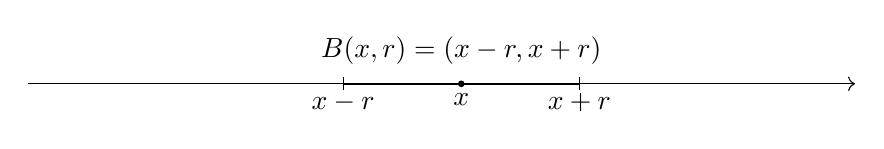
\begin{tikzpicture}[x=10cm,y=1cm]
  \draw[->] (0,0) -- (1.05,0);

  \coordinate (x) at (0.55,0);
  \coordinate (l) at (0.40,0);
  \coordinate (r) at (0.70,0);

  \fill (x) circle (1.2pt);
  
  % 修改 1: 直接连接两个坐标点，去掉括号里的 0
  \draw[thick] (l) -- (r);

  \node[below] at (x) {$x$};
  \node[below] at (l) {$x-r$};
  \node[below] at (r) {$x+r$};

  % 修改 2: 使用相对坐标画竖线
  % (l) ++(0,0.08) 意思是从 l 点向上走 0.08 开始画
  % -- ++(0,-0.16) 意思是接着向下画 0.16 (即画到 -0.08 的位置)
  \draw (l) ++(0,0.08) -- ++(0,-0.16);
  \draw (r) ++(0,0.08) -- ++(0,-0.16);
  
  \node[above] at (0.55,0.12) {$B(x,r)=(x-r,x+r)$};
\end{tikzpicture}
\caption{In $\RR$, an open ball is exactly an open interval centered at $x$.}
\end{figure}

\begin{proposition}[Basic closure properties of open sets]\label{prop:open-ops}
\begin{enumerate}[label=(\alph*)]
\item The union of any family of open sets is open.
\item The intersection of finitely many open sets is open.
\end{enumerate}
\end{proposition}

\begin{proof}
(a) Let $\{U_\alpha\}_{\alpha\in A}$ be open and set $U=\bigcup_{\alpha\in A}U_\alpha$.
Take $x\in U$. Then $x\in U_{\alpha_0}$ for some $\alpha_0$, and since $U_{\alpha_0}$ is open there exists $r>0$ with
$B(x,r)\subseteq U_{\alpha_0}\subseteq U$. Hence $U$ is open.

(b) Let $U_1,\dots,U_m$ be open and set $U=\bigcap_{j=1}^m U_j$.
Take $x\in U$. For each $j$ there exists $r_j>0$ such that $B(x,r_j)\subseteq U_j$.
Let $r=\min\{r_1,\dots,r_m\}>0$. Then $B(x,r)\subseteq U_j$ for all $j$, hence $B(x,r)\subseteq U$.
So $U$ is open.
\end{proof}

\subsubsection{Closed Sets and Equivalent Characterizations}

\begin{definition}[Closed set]\label{def:closed-set}
A set $F\subseteq \RR$ is \emph{closed} if its complement $\RR\setminus F$ is open.
\end{definition}

\begin{proposition}[Basic closure properties of closed sets]\label{prop:closed-ops}
\begin{enumerate}[label=(\alph*)]
\item The intersection of any family of closed sets is closed.
\item The union of finitely many closed sets is closed.
\end{enumerate}
\end{proposition}

\begin{proof}
This is immediate from \Cref{prop:open-ops} by taking complements and using De Morgan's laws.
\end{proof}

\begin{definition}[Limit point / accumulation point]\label{def:limit-point-set}
Let $A\subseteq\RR$. A point $x\in\RR$ is a \emph{limit point} of $A$ if for every $r>0$,
\[
\bigl(B(x,r)\setminus\{x\}\bigr)\cap A \neq \emptyset.
\]
Equivalently: every punctured neighborhood of $x$ contains a point of $A$.
\end{definition}

\begin{remark}
A limit point of $A$ need not belong to $A$.
For example, $0$ is a limit point of $(0,1)$, but $0\notin (0,1)$.
\end{remark}

\begin{theorem}[Closed sets contain their limit points]\label{thm:closed-limit-points}
A set $F\subseteq\RR$ is closed if and only if it contains all of its limit points.
\end{theorem}

\begin{proof}
($\Rightarrow$) Assume $F$ is closed and let $x$ be a limit point of $F$.
If $x\notin F$, then $x\in \RR\setminus F$, and since $\RR\setminus F$ is open, there exists $r>0$ with
$B(x,r)\subseteq \RR\setminus F$. This implies $B(x,r)\cap F=\emptyset$, contradicting that $x$ is a limit point of $F$.
Hence $x\in F$.

($\Leftarrow$) Assume $F$ contains all of its limit points. We show $\RR\setminus F$ is open.
Take $x\in \RR\setminus F$. If every ball $B(x,r)$ met $F$, then $x$ would be a limit point of $F$ (indeed, $B(x,r)\setminus\{x\}=B(x,r)$ since $x\notin F$),
hence $x\in F$ by assumption, a contradiction. Therefore, there exists $r>0$ with $B(x,r)\cap F=\emptyset$, i.e.\ $B(x,r)\subseteq \RR\setminus F$.
Thus $\RR\setminus F$ is open, and $F$ is closed.
\end{proof}

\subsubsection{Closure, Interior, and Boundary}

\begin{definition}[Closure]\label{def:closure}
For $A\subseteq \RR$, the \emph{closure} of $A$, denoted $\overline{A}$, is the intersection of all closed sets containing $A$:
\[
\overline{A} \coloneqq \bigcap\set{F\subseteq\RR:\ F\text{ closed and }A\subseteq F}.
\]
\end{definition}

\begin{proposition}[Basic facts about closure]\label{prop:closure-basic}
For any $A\subseteq\RR$:
\begin{enumerate}[label=(\alph*)]
\item $A\subseteq \overline{A}$ and $\overline{A}$ is closed.
\item $\overline{A}$ is the \emph{smallest} closed set containing $A$: if $F$ is closed and $A\subseteq F$, then $\overline{A}\subseteq F$.
\item $\overline{A}=A$ if and only if $A$ is closed.
\end{enumerate}
\end{proposition}

\begin{proof}
(a) Each closed superset $F$ of $A$ contains $A$, so the intersection contains $A$. Intersections of closed sets are closed (\Cref{prop:closed-ops}).

(b) If $F$ is closed with $A\subseteq F$, then $F$ appears in the intersection defining $\overline{A}$, so $\overline{A}\subseteq F$.

(c) If $A$ is closed, then by (a) and (b) we have $A\subseteq \overline{A}\subseteq A$, so $\overline{A}=A$.
Conversely, if $\overline{A}=A$, then $A$ is closed because $\overline{A}$ is closed by (a).
\end{proof}

\begin{theorem}[Characterizations of closure]\label{thm:closure-char}
Let $A\subseteq\RR$ and $x\in\RR$. The following are equivalent:
\begin{enumerate}[label=(\alph*)]
\item $x\in \overline{A}$.
\item For every $r>0$, $B(x,r)\cap A\neq \emptyset$.
\item There exists a sequence $(a_n)$ with $a_n\in A$ for all $n$ and $a_n\to x$.
\end{enumerate}
\end{theorem}

\begin{proof}
(a)$\Rightarrow$(b): If (b) fails, then for some $r>0$ we have $B(x,r)\cap A=\emptyset$.
Then $U\coloneqq B(x,r)$ is open and disjoint from $A$, so $\RR\setminus U$ is closed and contains $A$.
Hence $\overline{A}\subseteq \RR\setminus U$, so $x\notin \overline{A}$, contradicting (a).

(b)$\Rightarrow$(c): For each $n\in\NN$, apply (b) with $r=1/n$ to choose $a_n\in A\cap B(x,1/n)$.
Then $\abs{a_n-x}<1/n\to 0$, so $a_n\to x$.

(c)$\Rightarrow$(a): Let $F$ be any closed set with $A\subseteq F$.
Since $a_n\in A\subseteq F$ and $F$ is closed, \Cref{thm:closed-limit-points} implies the limit $x$ of $(a_n)$ lies in $F$.
This holds for every such $F$, hence $x\in\bigcap F=\overline{A}$.
\end{proof}

\begin{definition}[Interior]\label{def:interior}
For $A\subseteq\RR$, the \emph{interior} of $A$, denoted $\Int(A)$, is the set of points $x\in A$ for which there exists $r>0$ such that
\[
B(x,r)\subseteq A.
\]
Equivalently, $\Int(A)$ is the union of all open sets contained in $A$.
\end{definition}

\begin{proposition}[Basic facts about interior]\label{prop:interior-basic}
For any $A\subseteq\RR$:
\begin{enumerate}[label=(\alph*)]
\item $\Int(A)$ is open and $\Int(A)\subseteq A$.
\item $\Int(A)$ is the \emph{largest} open set contained in $A$: if $U$ is open and $U\subseteq A$, then $U\subseteq \Int(A)$.
\item $\Int(A)=A$ if and only if $A$ is open.
\end{enumerate}
\end{proposition}

\begin{proof}
(a) If $x\in\Int(A)$, there exists $r>0$ with $B(x,r)\subseteq A$.
But then for any $y\in B(x,r/2)$ we have $B(y,r/2)\subseteq B(x,r)\subseteq A$, so $y\in\Int(A)$.
Hence $B(x,r/2)\subseteq \Int(A)$ and $\Int(A)$ is open. Also $\Int(A)\subseteq A$ by definition.

(b) If $U$ is open and $U\subseteq A$, then for any $x\in U$ there exists $r>0$ with $B(x,r)\subseteq U\subseteq A$, so $x\in\Int(A)$.

(c) If $A$ is open, then every $x\in A$ has a ball contained in $A$, so $A\subseteq \Int(A)$; combined with (a), $\Int(A)=A$.
Conversely, if $\Int(A)=A$, then $A$ is open by (a).
\end{proof}

\begin{definition}[Boundary]\label{def:boundary}
For $A\subseteq\RR$, the \emph{boundary} of $A$ is
\[
\partial A \coloneqq \overline{A}\setminus \Int(A).
\]
\end{definition}

\begin{proposition}[Boundary characterizations]\label{prop:boundary-char}
Let $A\subseteq\RR$ and $x\in\RR$. The following are equivalent:
\begin{enumerate}[label=(\alph*)]
\item $x\in \partial A$.
\item For every $r>0$, both $B(x,r)\cap A\neq\emptyset$ and $B(x,r)\cap (\RR\setminus A)\neq\emptyset$.
\end{enumerate}
Moreover, $\partial A$ is closed.
\end{proposition}

\begin{proof}
(a)$\Leftrightarrow$(b):
$x\in\overline{A}$ is equivalent to $B(x,r)\cap A\neq\emptyset$ for all $r>0$ by \Cref{thm:closure-char}.
Also $x\notin \Int(A)$ means: for every $r>0$, $B(x,r)\nsubseteq A$, i.e.\ $B(x,r)\cap(\RR\setminus A)\neq\emptyset$.
Combining yields (b).

Closedness: since $\partial A=\overline{A}\cap (\Int(A))^c$ and $\overline{A}$ is closed while $\Int(A)$ is open, $(\Int(A))^c$ is closed.
Hence $\partial A$ is an intersection of closed sets, therefore closed.
\end{proof}

\begin{example}
Let $A=(0,1)\cup(2,3)$.
Then
\[
\Int(A)=A,\qquad
\overline{A}=[0,1]\cup[2,3],\qquad
\partial A=\{0,1,2,3\}.
\]
\end{example}

\begin{figure}[H]
\centering
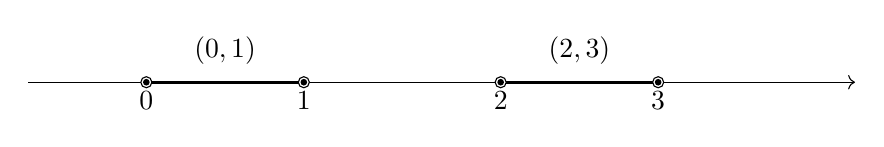
\begin{tikzpicture}[x=10cm,y=1cm]
  \draw[->] (0,0) -- (1.05,0);

  % map real points to positions
  \coordinate (z0) at (0.15,0); % 0
  \coordinate (z1) at (0.35,0); % 1
  \coordinate (z2) at (0.60,0); % 2
  \coordinate (z3) at (0.80,0); % 3

  % interior parts (open intervals)
  \draw[very thick] (0.15,0) -- (0.35,0);
  \draw[very thick] (0.60,0) -- (0.80,0);

  % open endpoints (draw as white circles on top)
  \fill[white] (z0) circle (2.0pt);
  \fill[white] (z1) circle (2.0pt);
  \fill[white] (z2) circle (2.0pt);
  \fill[white] (z3) circle (2.0pt);
  \draw (z0) circle (2.0pt);
  \draw (z1) circle (2.0pt);
  \draw (z2) circle (2.0pt);
  \draw (z3) circle (2.0pt);

  % boundary points highlighted below
  \fill (z0) circle (1.2pt);
  \fill (z1) circle (1.2pt);
  \fill (z2) circle (1.2pt);
  \fill (z3) circle (1.2pt);

  \node[below] at (z0) {$0$};
  \node[below] at (z1) {$1$};
  \node[below] at (z2) {$2$};
  \node[below] at (z3) {$3$};

  \node[above] at (0.25,0.10) {$(0,1)$};
  \node[above] at (0.70,0.10) {$(2,3)$};
\end{tikzpicture}
\caption{For $A=(0,1)\cup(2,3)$, the boundary is $\{0,1,2,3\}$ and the closure adds endpoints.}
\end{figure}

\subsubsection{Subspace Topology (Relative Openness/Closedness)}

\begin{definition}[Open in a subset / relative topology]\label{def:relative-open}
Let $E\subseteq\RR$ and $U\subseteq E$.
We say $U$ is \emph{open in $E$} (or \emph{relatively open}) if there exists an open set $V\subseteq\RR$ such that
\[
U = E\cap V.
\]
Similarly, $F\subseteq E$ is \emph{closed in $E$} if there exists a closed set $C\subseteq\RR$ such that $F=E\cap C$,
equivalently if $E\setminus F$ is open in $E$.
\end{definition}

\begin{example}
In $E=[0,1]$, the set $[0,\tfrac12)$ is open in $E$ because
\[
[0,\tfrac12) = [0,1]\cap (-1,\tfrac12).
\]
But $[0,\tfrac12)$ is not open in $\RR$.
\end{example}

\begin{exercise}
Prove that for $A\subseteq\RR$,
\[
\overline{A} = \RR \setminus \Int(\RR\setminus A).
\]
(Hint: use the ball characterizations of closure and interior.)
\end{exercise}

\begin{exercise}
Let $A\subseteq\RR$. Show that $\overline{A}$ is the set of all limits of sequences from $A$ (allowing eventually constant sequences).
Show that $x$ is a limit point of $A$ if and only if there exists a sequence $(a_n)$ with $a_n\in A\setminus\{x\}$ and $a_n\to x$.
\end{exercise}

\newpage

% -------------------------------------------------
\subsection{Compactness}

\subsubsection{Open Covers and Compact Sets}

\begin{definition}[Open cover]
Let $K\subseteq\RR$. A family $\{U_\alpha\}_{\alpha\in A}$ of open sets in $\RR$ is an \emph{open cover} of $K$ if
\[
K \subseteq \bigcup_{\alpha\in A} U_\alpha.
\]
A \emph{finite subcover} is a finite subcollection $U_{\alpha_1},\dots,U_{\alpha_m}$ such that
\[
K \subseteq \bigcup_{j=1}^{m} U_{\alpha_j}.
\]
\end{definition}

\begin{definition}[Compactness]\label{def:compact}
A set $K\subseteq\RR$ is \emph{compact} if every open cover of $K$ has a finite subcover.
\end{definition}

\begin{remark}
Compactness is a finiteness principle: it says that even though $K$ may be infinite, any attempt to cover it by open sets can be reduced to finitely many of them.
On $\RR$, compactness will turn out to be exactly the same as being \emph{closed and bounded} (Heine--Borel).
\end{remark}

\subsubsection{Compactness of Closed Intervals}

\begin{theorem}[Heine--Borel for intervals]\label{thm:interval-compact}
Every closed interval $[a,b]\subseteq\RR$ is compact.
\end{theorem}

\begin{proof}
Let $\{U_\alpha\}_{\alpha\in A}$ be an open cover of $[a,b]$.
Define
\[
S \coloneqq \set{x\in[a,b] : [a,x]\ \text{can be covered by finitely many }U_\alpha }.
\]
We prove $b\in S$, which is exactly the statement that $[a,b]$ has a finite subcover.

\medskip
\noindent\textbf{Step 1: $S$ is nonempty.}
Since $\{U_\alpha\}$ covers $[a,b]$, there exists $\alpha_0$ with $a\in U_{\alpha_0}$.
Because $U_{\alpha_0}$ is open, there exists $\delta>0$ such that $B(a,\delta)\subseteq U_{\alpha_0}$.
Then $[a,\min\{a+\delta/2,b\}]\subseteq U_{\alpha_0}$, so $\min\{a+\delta/2,b\}\in S$.
Hence $S\neq\emptyset$.

\medskip
\noindent\textbf{Step 2: Let $c=\sup S$. Then $c=b$.}
Since $S\subseteq[a,b]$, it is bounded above, hence $c=\sup S$ exists.
Assume for contradiction that $c<b$.

Because $\{U_\alpha\}$ covers $[a,b]$, pick $\beta$ such that $c\in U_\beta$.
Since $U_\beta$ is open, choose $\eta>0$ with $B(c,\eta)\subseteq U_\beta$.

By the supremum approximation property, there exists $x\in S$ such that
\[
c-\frac{\eta}{2} < x \le c.
\]
By definition of $S$, the interval $[a,x]$ is covered by finitely many sets from the family, say
\[
[a,x] \subseteq U_{\alpha_1}\cup\cdots\cup U_{\alpha_m}.
\]
Also, since $x>c-\eta/2$, we have
\[
[x,\,c+\eta/2] \subseteq [c-\eta/2,\,c+\eta/2]\subseteq B(c,\eta)\subseteq U_\beta.
\]
Therefore,
\[
[a,\,c+\eta/2] \subseteq U_{\alpha_1}\cup\cdots\cup U_{\alpha_m}\cup U_\beta,
\]
which is a finite subcover of $[a,c+\eta/2]$.
Hence $c+\eta/2\in S$, contradicting that $c$ is an upper bound of $S$.
Thus $c=b$.

\medskip
\noindent\textbf{Step 3: Conclude $b\in S$.}
Since $c=\sup S=b$ and $b\in[a,b]$, the definition of $S$ implies $[a,b]$ has a finite subcover.
Therefore $[a,b]$ is compact.
\end{proof}

\subsubsection{Closed Subsets of Compact Sets}

\begin{theorem}[Closed subset of compact is compact]\label{thm:closed-subset-compact}
If $K\subseteq\RR$ is compact and $F\subseteq K$ is closed in $\RR$, then $F$ is compact.
\end{theorem}

\begin{proof}
Let $\{U_\alpha\}_{\alpha\in A}$ be an open cover of $F$ (open in $\RR$).
Since $F$ is closed, $\RR\setminus F$ is open. Then
\[
K \subseteq \Bigl(\bigcup_{\alpha\in A} U_\alpha\Bigr)\cup (\RR\setminus F),
\]
so $\{U_\alpha\}_{\alpha\in A}\cup\{\RR\setminus F\}$ is an open cover of $K$.
By compactness of $K$, there exists a finite subcover:
\[
K \subseteq U_{\alpha_1}\cup\cdots\cup U_{\alpha_m}\cup(\RR\setminus F).
\]
Intersecting both sides with $F$ eliminates $\RR\setminus F$ and yields
\[
F \subseteq U_{\alpha_1}\cup\cdots\cup U_{\alpha_m}.
\]
Thus $F$ has a finite subcover and is compact.
\end{proof}

\subsubsection{Compact Sets Are Closed and Bounded}

\begin{theorem}[Compact $\Rightarrow$ bounded]\label{thm:compact-bounded}
If $K\subseteq\RR$ is compact, then $K$ is bounded.
\end{theorem}

\begin{proof}
For each $n\in\NN$, the open interval $(-n,n)$ is open and
\[
\RR = \bigcup_{n\in\NN} (-n,n).
\]
Hence $\{(-n,n)\}_{n\in\NN}$ is an open cover of $K$.
By compactness, there exists $n_1,\dots,n_m$ such that
\[
K \subseteq \bigcup_{j=1}^m (-n_j,n_j).
\]
Let $N=\max\{n_1,\dots,n_m\}$. Then $\bigcup_{j=1}^m (-n_j,n_j)\subseteq (-N,N)$, so $K\subseteq (-N,N)$ and $K$ is bounded.
\end{proof}

\begin{theorem}[Compact $\Rightarrow$ closed]\label{thm:compact-closed}
If $K\subseteq\RR$ is compact, then $K$ is closed.
\end{theorem}

\begin{proof}
We show that $\RR\setminus K$ is open.
Let $x\in \RR\setminus K$. For each $y\in K$, define
\[
r_y \coloneqq \frac{\abs{x-y}}{2} > 0,
\qquad
V_y \coloneqq B(y,r_y).
\]
Then $V_y$ is open, $y\in V_y$, and importantly $x\notin V_y$ (since $\abs{x-y}=2r_y$).
The family $\{V_y\}_{y\in K}$ is an open cover of $K$, so by compactness there exist $y_1,\dots,y_m\in K$ such that
\[
K \subseteq V_{y_1}\cup\cdots\cup V_{y_m}.
\]
Let
\[
r \coloneqq \min\{r_{y_1},\dots,r_{y_m}\} > 0.
\]
We claim that $B(x,r)\cap K=\emptyset$.

Indeed, take any $z\in B(x,r)$. For each $j$,
\[
\abs{z-y_j} \ge \abs{x-y_j} - \abs{z-x} > \abs{x-y_j} - r \ge \abs{x-y_j} - r_{y_j} = r_{y_j},
\]
so $z\notin V_{y_j}$.
Thus $z\notin \bigcup_{j=1}^m V_{y_j}$, and since $K\subseteq \bigcup_{j=1}^m V_{y_j}$, we must have $z\notin K$.
Therefore $B(x,r)\subseteq \RR\setminus K$, showing $\RR\setminus K$ is open.
Hence $K$ is closed.
\end{proof}

\subsubsection{Heine--Borel Theorem}

\begin{theorem}[Heine--Borel on $\RR$]\label{thm:heine-borel-R}
A subset $K\subseteq\RR$ is compact if and only if it is closed and bounded.
\end{theorem}

\begin{proof}
($\Rightarrow$) If $K$ is compact, then it is bounded by \Cref{thm:compact-bounded} and closed by \Cref{thm:compact-closed}.

($\Leftarrow$) If $K$ is closed and bounded, then $K\subseteq [a,b]$ for some $a<b$.
By \Cref{thm:interval-compact}, $[a,b]$ is compact. Since $K$ is closed in $\RR$, it is a closed subset of $[a,b]$ as well,
hence $K$ is compact by \Cref{thm:closed-subset-compact}.
\end{proof}

\subsubsection{Sequential Compactness}

\begin{definition}[Sequential compactness]\label{def:sequential-compact}
A set $K\subseteq\RR$ is \emph{sequentially compact} if every sequence in $K$ has a subsequence that converges to a point in $K$.
\end{definition}

\begin{theorem}[Compactness and sequential compactness on $\RR$]\label{thm:compact-seqcompact}
For $K\subseteq\RR$, the following are equivalent:
\begin{enumerate}[label=(\alph*)]
\item $K$ is compact.
\item $K$ is sequentially compact.
\item $K$ is closed and bounded.
\end{enumerate}
\end{theorem}

\begin{proof}
(a)$\Rightarrow$(c) is \Cref{thm:compact-bounded,thm:compact-closed}, and (c)$\Rightarrow$(a) is \Cref{thm:heine-borel-R}.

(c)$\Rightarrow$(b): If $K$ is bounded, then any sequence in $K$ is bounded, so by Bolzano--Weierstrass it has a convergent subsequence in $\RR$.
If $K$ is also closed, the limit of that subsequence must lie in $K$ (closed sets contain limits of convergent sequences). Thus $K$ is sequentially compact.

(b)$\Rightarrow$(c): If $K$ were unbounded, we could choose $x_n\in K$ with $\abs{x_n}\ge n$.
Then $(x_n)$ has no convergent subsequence (any convergent subsequence must be bounded), contradicting sequential compactness.
So $K$ is bounded.

To see $K$ is closed, let $(x_n)$ be a sequence in $K$ with $x_n\to x\in\RR$.
By sequential compactness, $(x_n)$ has a subsequence $x_{n_k}\to y$ with $y\in K$.
But a subsequence of a convergent sequence converges to the same limit, so $y=x$.
Hence $x\in K$, showing $K$ is closed.
\end{proof}

\begin{exercise}
Show that a set $K\subseteq\RR$ is compact if and only if every sequence in $K$ has a Cauchy subsequence.
Then explain why completeness of $\RR$ upgrades this to an actually convergent subsequence.
\end{exercise}

\begin{exercise}
Give an example of a closed set in $\RR$ that is not compact, and explain precisely which hypothesis in Heine--Borel fails.
\end{exercise}

\newpage

% -------------------------------------------------
\subsection{Connectedness}

\subsubsection{Connected Sets and Separations}

\begin{definition}[Separation and connectedness]\label{def:connected}
Let $E\subseteq\RR$.
A \emph{separation} of $E$ is a pair of sets $A,B\subseteq E$ such that:
\begin{enumerate}[label=(\roman*)]
\item $A\neq\emptyset$ and $B\neq\emptyset$,
\item $A\cap B=\emptyset$ and $E=A\cup B$,
\item $A$ and $B$ are open in the relative topology on $E$ (equivalently, open subsets of $E$).
\end{enumerate}
We say $E$ is \emph{connected} if it admits no separation.
\end{definition}

\begin{remark}
Connectedness is the formal version of ``$E$ has no gaps.'' On $\RR$, it will be equivalent to $E$ being an interval (possibly a single point).
\end{remark}

\begin{definition}[Clopen sets in a subspace]
A subset $U\subseteq E$ is \emph{clopen in $E$} if it is both open in $E$ and closed in $E$.
\end{definition}

\begin{proposition}[Connectedness via clopen sets]\label{prop:clopen}
A set $E\subseteq\RR$ is connected if and only if the only clopen subsets of $E$ are $\emptyset$ and $E$ itself.
\end{proposition}

\begin{proof}
If $E$ has a separation $E=A\cup B$ with $A,B$ nonempty disjoint and open in $E$, then $A=E\setminus B$ so $A$ is also closed in $E$.
Thus $A$ is a nontrivial clopen subset.

Conversely, if $U\subseteq E$ is nonempty and not all of $E$ and is clopen in $E$, then $E=U\cup(E\setminus U)$ is a separation
because $U$ and $E\setminus U$ are disjoint, nonempty, and open in $E$ (since $U$ is closed in $E$ implies $E\setminus U$ is open in $E$).
\end{proof}

\subsubsection{Intervals as Connected Sets}

\begin{definition}[Interval]
A set $I\subseteq\RR$ is an \emph{interval} if for all $a,b\in I$ with $a<b$, every $c$ with $a<c<b$ also lies in $I$.
Equivalently,
\[
a,b\in I,\ a<b \quad\Rightarrow\quad (a,b)\subseteq I.
\]
\end{definition}

\begin{theorem}[Intervals are connected]\label{thm:interval-connected}
Every interval $I\subseteq\RR$ is connected.
\end{theorem}

\begin{proof}
Assume for contradiction that $I$ is an interval and $I=A\cup B$ is a separation with $A,B$ nonempty, disjoint, and open in $I$.
Choose $a\in A$ and $b\in B$. WLOG assume $a<b$ (otherwise swap $A,B$).

Define
\[
S \coloneqq A\cap [a,b] \subseteq [a,b].
\]
Then $S$ is nonempty (since $a\in S$) and bounded above by $b$, so $c=\sup S$ exists with $a\le c\le b$.

We show $c\notin A$ and $c\notin B$, a contradiction because $I=A\cup B$.

\medskip
\noindent\textbf{Claim 1: $c\notin A$.}
If $c\in A$, since $A$ is open in $I$, there exists $\eps>0$ such that
\[
I\cap (c-\eps,c+\eps)\subseteq A.
\]
Because $c\le b$, the point $c'=\min\{c+\eps/2,b\}$ belongs to $I\cap (c-\eps,c+\eps)$ and hence to $A$.
Moreover, $c'\in [a,b]$ and $c'>c$, so $c'\in S$ with $c'>c$, contradicting that $c$ is an upper bound of $S$.
Thus $c\notin A$.

\medskip
\noindent\textbf{Claim 2: $c\notin B$.}
If $c\in B$, since $B$ is open in $I$, there exists $\eps>0$ such that
\[
I\cap (c-\eps,c+\eps)\subseteq B.
\]
By definition of supremum, there exists $s\in S$ with $c-\eps/2 < s \le c$.
Then $s\in A$ and also $s\in I\cap (c-\eps,c+\eps)$, so $s\in B$ as well.
This contradicts $A\cap B=\emptyset$. Hence $c\notin B$.

Therefore $c\notin A\cup B=I$, impossible since $c\in[a,b]\subseteq I$ (because $I$ is an interval containing $a$ and $b$).
So no separation exists and $I$ is connected.
\end{proof}

\subsubsection{Connected Subsets of $\RR$ Are Intervals}

\begin{theorem}[Connected $\Leftrightarrow$ interval in $\RR$]\label{thm:connected-interval}
A set $E\subseteq\RR$ is connected if and only if it is an interval (possibly a single point).
\end{theorem}

\begin{proof}
($\Leftarrow$) If $E$ is an interval, it is connected by \Cref{thm:interval-connected}.

($\Rightarrow$) Assume $E$ is connected.
Take $a,b\in E$ with $a<b$ and let $c$ satisfy $a<c<b$.
If $c\notin E$, then
\[
E = \bigl(E\cap(-\infty,c)\bigr)\ \cup\ \bigl(E\cap(c,\infty)\bigr),
\]
a disjoint union. Both pieces are open in $E$ (they are intersections of $E$ with open sets of $\RR$),
both are nonempty (they contain $a$ and $b$ respectively), and they cover $E$.
This is a separation of $E$, contradicting connectedness. Hence $c\in E$.
Therefore $(a,b)\subseteq E$, so $E$ is an interval.
\end{proof}

\subsubsection{Intermediate Value Property for Sets}

\begin{proposition}[Intermediate value property for connected sets]\label{prop:ivp-sets}
Let $E\subseteq\RR$. The following are equivalent:
\begin{enumerate}[label=(\alph*)]
\item $E$ is connected.
\item Whenever $a,b\in E$ with $a<b$, then every $c$ with $a\le c\le b$ lies in $E$.
\end{enumerate}
\end{proposition}

\begin{proof}
This is exactly \Cref{thm:connected-interval}, noting that including endpoints corresponds to the same interval property stated with $\le$.
\end{proof}

\begin{remark}
Later, we will prove that continuous functions map connected sets to connected sets.
Combining that with \Cref{prop:ivp-sets} yields the Intermediate Value Theorem for continuous functions on intervals.
\end{remark}

\subsubsection{Connected Components}

\begin{definition}[Connected component]\label{def:component}
Let $E\subseteq\RR$ and $x\in E$.
The \emph{connected component of $x$ in $E$} is the union of all connected subsets of $E$ that contain $x$.
\end{definition}

\begin{theorem}[Components partition the set]\label{thm:components-partition}
The connected components of $E$ form a partition of $E$:
\begin{enumerate}[label=(\alph*)]
\item Every $x\in E$ lies in exactly one connected component.
\item Distinct connected components are disjoint.
\end{enumerate}
Moreover, each component is connected and is maximal among connected subsets of $E$ (by inclusion).
\end{theorem}

\begin{proof}
Fix $x\in E$ and let $C_x$ be the union of all connected subsets of $E$ containing $x$.
Then $C_x$ is connected: if it had a separation, restricting to any connected subset containing $x$ would produce a separation there, impossible.
(Equivalently: unions of connected sets with nonempty intersection are connected; here all sets intersect at $x$.)

If $y\in C_x$, then $C_y=C_x$ because any connected set containing $y$ and contained in $E$ can be joined (via union) with a connected set containing $x$ and $y$ inside $C_x$,
forcing both maximal unions to coincide. Hence components either coincide or are disjoint, so they partition $E$.
Maximality follows directly from the definition: any connected subset of $E$ containing $x$ is contained in the union $C_x$.
\end{proof}

\begin{corollary}[Components in $\RR$ are intervals]\label{cor:components-intervals}
If $E\subseteq\RR$, then each connected component of $E$ is an interval (possibly a single point).
\end{corollary}

\begin{proof}
Each component is a connected subset of $\RR$, hence an interval by \Cref{thm:connected-interval}.
\end{proof}

\begin{example}
Let $E=(-1,0)\cup(1,3]\cup\{5\}$.
Then $E$ has three connected components: $(-1,0)$, $(1,3]$, and $\{5\}$.
\end{example}

\begin{figure}[H]
\centering
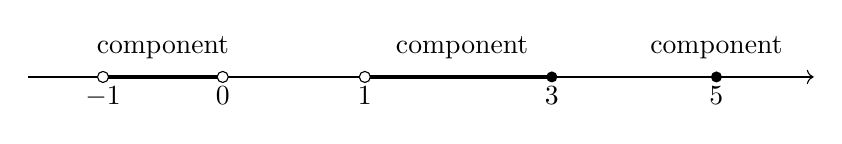
\begin{tikzpicture}[x=9.5cm,y=1cm]
  \draw[->] (0,0) -- (1.05,0);

  % positions
  \coordinate (m1) at (0.10,0); % -1
  \coordinate (z0) at (0.26,0); % 0
  \coordinate (p1) at (0.45,0); % 1
  \coordinate (p3) at (0.70,0); % 3
  \coordinate (p5) at (0.92,0); % 5

  % (-1,0)
  % 修改1：去掉多余的 ,0，直接连接坐标点
  \draw[very thick] (m1) -- (z0); 
  
  \fill[white] (m1) circle (2.0pt); \draw (m1) circle (2.0pt);
  \fill[white] (z0) circle (2.0pt); \draw (z0) circle (2.0pt);

  % (1,3]
  % 修改2：同上，直接使用 (p1) -- (p3)
  \draw[very thick] (p1) -- (p3);
  
  \fill[white] (p1) circle (2.0pt); \draw (p1) circle (2.0pt);
  \fill (p3) circle (2.0pt); % closed endpoint at 3

  % {5}
  \fill (p5) circle (2.0pt);

  \node[below] at (m1) {$-1$};
  \node[below] at (z0) {$0$};
  \node[below] at (p1) {$1$};
  \node[below] at (p3) {$3$};
  \node[below] at (p5) {$5$};

  \node[above] at (0.18,0.10) {component};
  \node[above] at (0.58,0.10) {component};
  \node[above] at (0.92,0.10) {component};
\end{tikzpicture}
\caption{Connected components in $\RR$ are precisely the ``maximal pieces with no gaps'' (intervals or points).}
\end{figure}

\begin{exercise}
Prove directly from the definition that if $E\subseteq\RR$ is connected and $f:E\to\RR$ is continuous (definition later),
then $f(E)$ is connected. Explain how this implies the Intermediate Value Theorem.
\end{exercise}

\begin{exercise}
Let $A\subseteq\RR$. Prove that $\overline{A}$ is connected whenever $A$ is connected.
(Hint: use \Cref{thm:connected-interval}.)
\end{exercise}

\begin{exercise}
Let $E\subseteq\RR$ and let $\{C_i\}_{i\in I}$ be its connected components.
Show that each $C_i$ is closed in $E$ (relative topology).
Is each $C_i$ necessarily open in $E$? Give a criterion or counterexample.
\end{exercise}

\newpage

% =========================
% Continuity
% =========================

\section{Continuity}

\begin{keyidea}
Continuity is the rigorous formulation of ``small changes in input produce small changes in output.''
There are multiple equivalent ways to express continuity:
\begin{itemize}
\item $\eps$--$\delta$ definition (local control),
\item sequential characterization (continuity preserves limits of sequences),
\item topological characterization (preimages of open/closed sets).
\end{itemize}
On $\RR$, these viewpoints are equivalent and each is useful in different proofs.
\end{keyidea}

% -------------------------------------------------
\subsection{The \texorpdfstring{$\eps$--$\delta$}{epsilon-delta} Definition}

\subsubsection{Continuity at a Point}

\begin{definition}[Continuity at a point]\label{def:cont-point}
Let $f:D\to\RR$ with $D\subseteq\RR$, and let $a\in D$.
We say $f$ is \emph{continuous at $a$} if
\[
\forall \eps>0\ \exists \delta>0\ \forall x\in D,\quad \abs{x-a}<\delta \Rightarrow \abs{f(x)-f(a)}<\eps.
\]
If $f$ is continuous at every $a\in D$, we say $f$ is \emph{continuous on $D$}.
\end{definition}

\begin{remark}[Domain matters]
The quantifier ``for all $x$'' is restricted to $x\in D$.
Continuity at a boundary point of $D$ is therefore a one-sided phenomenon automatically built into the definition.
For example, $f(x)=\sqrt{x}$ is continuous at $0$ as a function on $D=[0,\infty)$.
\end{remark}

\subsubsection{Equivalent ``Neighborhood'' Formulation}

\begin{proposition}[Ball formulation]\label{prop:cont-ball}
Let $f:D\to\RR$ and $a\in D$. Then $f$ is continuous at $a$ if and only if:
for every $r>0$ there exists $\delta>0$ such that
\[
f\bigl(B(a,\delta)\cap D\bigr)\subseteq B(f(a),r).
\]
\end{proposition}

\begin{proof}
This is a direct rewriting of \Cref{def:cont-point} with $r=\eps$ and the notation $B(\cdot,\cdot)$ for open balls in $\RR$.
\end{proof}

\subsubsection{Examples and Non-Examples}

\begin{example}[Constant and identity functions]
If $f(x)=c$, then $\abs{f(x)-f(a)}=0<\eps$ for all $x$, so any $\delta>0$ works; hence $f$ is continuous everywhere.
If $f(x)=x$, then $\abs{f(x)-f(a)}=\abs{x-a}$, so choosing $\delta=\eps$ proves continuity.
\end{example}

\begin{example}[Linear functions]
Let $f(x)=mx+b$. Fix $a\in\RR$ and $\eps>0$.
Then
\[
\abs{f(x)-f(a)}=\abs{m(x-a)}=\abs{m}\abs{x-a}.
\]
If $m=0$, $f$ is constant. If $m\neq 0$, choosing $\delta=\eps/\abs{m}$ yields $\abs{f(x)-f(a)}<\eps$ whenever $\abs{x-a}<\delta$.
Thus every linear function is continuous on $\RR$.
\end{example}

\begin{example}[Quadratic function]
Let $f(x)=x^2$. Fix $a\in\RR$.
We estimate
\[
\abs{x^2-a^2}=\abs{x-a}\abs{x+a}.
\]
To control $\abs{x+a}$, impose $\abs{x-a}<1$ so that $\abs{x}\le \abs{a}+1$ and hence
\[
\abs{x+a}\le \abs{x}+\abs{a}\le 2\abs{a}+1.
\]
Given $\eps>0$, choose
\[
\delta=\min\left\{1,\ \frac{\eps}{2\abs{a}+1}\right\}.
\]
Then $\abs{x-a}<\delta$ implies
\[
\abs{x^2-a^2}=\abs{x-a}\abs{x+a}<\delta(2\abs{a}+1)\le \eps,
\]
so $x^2$ is continuous at $a$.
\end{example}

\begin{example}[A discontinuous function: step function]
Define $f:\RR\to\RR$ by
\[
f(x)=
\casesm{
0, & x<0,\\
1, & x\ge 0.
}
\]
Then $f$ is discontinuous at $0$.
Indeed, take $\eps=\tfrac12$. For any $\delta>0$, choose $x=-\delta/2$ (so $\abs{x-0}<\delta$) but then
\[
\abs{f(x)-f(0)}=\abs{0-1}=1\ge \tfrac12,
\]
so the $\eps$--$\delta$ condition fails.
However, $f$ is continuous at every $a\neq 0$.
\end{example}

\begin{figure}[H]
\centering
\begin{tikzpicture}[x=7.5cm,y=2.2cm]
  \draw[->] (-0.05,0) -- (1.05,0) node[right] {$x$};
  \draw[->] (0,-0.05) -- (0,1.05) node[above] {$f(x)$};

  % map x from [-1,1] to [0,1] scale: use coordinate transform manually
  % draw horizontal segments: y=0 for x<0, y=1 for x>=0
  \draw[very thick] (0.05,0.20) -- (0.50,0.20); % left part (x<0)
  \draw[very thick] (0.50,0.80) -- (0.98,0.80); % right part (x>=0)

  % jump at 0: open circle at (0,0), closed at (0,1)
  \fill[white] (0.50,0.20) circle (2.1pt);
  \draw (0.50,0.20) circle (2.1pt);
  \fill (0.50,0.80) circle (2.1pt);

  \node[below] at (0.50,0) {$0$};
  \node[left] at (0,0.20) {$0$};
  \node[left] at (0,0.80) {$1$};

  \node at (0.78,0.92) {$f(x)=\mathbf{1}_{[0,\infty)}(x)$};
\end{tikzpicture}
\caption{A jump discontinuity at $x=0$: no matter how small $\delta$ is, values on both sides appear.}
\end{figure}

\subsubsection{Algebra of Continuous Functions}

\begin{theorem}[Algebraic operations preserve continuity]\label{thm:cont-algebra}
Let $f,g:D\to\RR$ be continuous at $a\in D$.
Then:
\begin{enumerate}[label=(\alph*)]
\item $f+g$ is continuous at $a$.
\item $fg$ is continuous at $a$.
\item If $g(a)\neq 0$, then $\frac{f}{g}$ is continuous at $a$ (on points where $g\neq 0$).
\item If $c\in\RR$, then $cf$ is continuous at $a$.
\end{enumerate}
\end{theorem}

\begin{proof}
Fix $\eps>0$.
\begin{enumerate}[label=(\alph*)]
\item Since $f$ and $g$ are continuous at $a$, there exist $\delta_1,\delta_2>0$ such that
$\abs{x-a}<\delta_1\Rightarrow \abs{f(x)-f(a)}<\eps/2$ and
$\abs{x-a}<\delta_2\Rightarrow \abs{g(x)-g(a)}<\eps/2$.
Let $\delta=\min\{\delta_1,\delta_2\}$. Then for $\abs{x-a}<\delta$,
\[
\abs{(f+g)(x)-(f+g)(a)}\le \abs{f(x)-f(a)}+\abs{g(x)-g(a)}<\eps.
\]

\item First note that continuity of $f$ at $a$ implies $f$ is bounded in a neighborhood of $a$:
take $\eta=1$ and choose $\delta_0>0$ such that $\abs{x-a}<\delta_0\Rightarrow \abs{f(x)-f(a)}<1$.
Then $\abs{f(x)}\le \abs{f(a)}+1$ whenever $\abs{x-a}<\delta_0$.

Now write
\[
f(x)g(x)-f(a)g(a)
= f(x)\bigl(g(x)-g(a)\bigr)+g(a)\bigl(f(x)-f(a)\bigr).
\]
Let $M=\abs{f(a)}+1$.
Choose $\delta_1>0$ such that $\abs{x-a}<\delta_1\Rightarrow \abs{f(x)-f(a)}<\eps/(2(\abs{g(a)}+1))$,
and choose $\delta_2>0$ such that $\abs{x-a}<\delta_2\Rightarrow \abs{g(x)-g(a)}<\eps/(2M)$.
Let $\delta=\min\{\delta_0,\delta_1,\delta_2\}$.
Then for $\abs{x-a}<\delta$ we have $\abs{f(x)}\le M$ and
\begin{align*}
\abs{f(x)g(x)-f(a)g(a)}
&\le \abs{f(x)}\abs{g(x)-g(a)}+\abs{g(a)}\abs{f(x)-f(a)}\\
&< M\cdot \frac{\eps}{2M} + \abs{g(a)}\cdot \frac{\eps}{2(\abs{g(a)}+1)}
\le \frac{\eps}{2}+\frac{\eps}{2}=\eps.
\end{align*}

\item Since $g(a)\neq 0$, let $\eta=\abs{g(a)}/2>0$.
By continuity of $g$, choose $\delta_0>0$ such that $\abs{x-a}<\delta_0\Rightarrow \abs{g(x)-g(a)}<\eta$.
Then $\abs{g(x)}\ge \abs{g(a)}-\eta=\abs{g(a)}/2$ for $\abs{x-a}<\delta_0$,
so $1/g(x)$ is well-defined and bounded there.

We show $1/g$ is continuous at $a$:
\[
\left|\frac{1}{g(x)}-\frac{1}{g(a)}\right|
=\frac{\abs{g(x)-g(a)}}{\abs{g(x)}\abs{g(a)}}
\le \frac{2}{\abs{g(a)}^2}\abs{g(x)-g(a)}
\quad (\abs{x-a}<\delta_0).
\]
Given $\eps>0$, choose $\delta_1>0$ so that $\abs{x-a}<\delta_1\Rightarrow
\abs{g(x)-g(a)}<\frac{\eps\abs{g(a)}^2}{2}$.
Then for $\abs{x-a}<\min\{\delta_0,\delta_1\}$ we have
$\abs{\frac{1}{g(x)}-\frac{1}{g(a)}}<\eps$.
Hence $1/g$ is continuous at $a$.

Finally, $\frac{f}{g}=f\cdot (1/g)$, and products of continuous functions are continuous by (b).

\item Immediate from $\abs{cf(x)-cf(a)}=\abs{c}\,\abs{f(x)-f(a)}$.
\end{enumerate}
\end{proof}

\subsubsection{Composition}

\begin{theorem}[Continuity of composition]\label{thm:cont-composition}
Let $f:D\to\RR$ and $g:E\to\RR$ with $f(D)\subseteq E$.
If $f$ is continuous at $a\in D$ and $g$ is continuous at $f(a)\in E$, then $g\circ f$ is continuous at $a$.
\end{theorem}

\begin{proof}
Let $\eps>0$. Since $g$ is continuous at $f(a)$, there exists $\eta>0$ such that
\[
\abs{y-f(a)}<\eta \Rightarrow \abs{g(y)-g(f(a))}<\eps.
\]
Since $f$ is continuous at $a$, there exists $\delta>0$ such that
\[
\abs{x-a}<\delta \Rightarrow \abs{f(x)-f(a)}<\eta.
\]
Therefore, if $\abs{x-a}<\delta$, then with $y=f(x)$ we have $\abs{y-f(a)}<\eta$ and hence
\[
\abs{g(f(x))-g(f(a))}<\eps.
\]
Thus $g\circ f$ is continuous at $a$.
\end{proof}

\begin{exercise}
Prove that polynomials are continuous on $\RR$ and rational functions are continuous on their domains.
(Hint: use \Cref{thm:cont-algebra} inductively.)
\end{exercise}

\newpage

% -------------------------------------------------
\subsection{Sequential Characterization of Continuity}

\subsubsection{Continuity Preserves Limits of Sequences}

\begin{theorem}[Sequential criterion]\label{thm:cont-seq}
Let $f:D\to\RR$ and $a\in D$.
Then $f$ is continuous at $a$ if and only if for every sequence $(x_n)$ in $D$ with $x_n\to a$, we have
\[
f(x_n)\to f(a).
\]
\end{theorem}

\begin{proof}
($\Rightarrow$) Assume $f$ is continuous at $a$ and let $x_n\to a$ with $x_n\in D$.
Let $\eps>0$. By continuity, choose $\delta>0$ such that $\abs{x-a}<\delta\Rightarrow \abs{f(x)-f(a)}<\eps$.
Since $x_n\to a$, there exists $N$ such that $n\ge N\Rightarrow \abs{x_n-a}<\delta$.
Then $n\ge N$ implies $\abs{f(x_n)-f(a)}<\eps$, so $f(x_n)\to f(a)$.

($\Leftarrow$) Assume the sequential property holds, and suppose for contradiction that $f$ is not continuous at $a$.
Then there exists $\eps_0>0$ such that for every $\delta>0$ there exists $x\in D$ with
\[
\abs{x-a}<\delta
\quad\text{and}\quad
\abs{f(x)-f(a)}\ge \eps_0.
\]
For each $n\in\NN$, apply this with $\delta=1/n$ to choose $x_n\in D$ such that
\[
\abs{x_n-a}<\frac{1}{n}
\quad\text{and}\quad
\abs{f(x_n)-f(a)}\ge \eps_0.
\]
Then $x_n\to a$, but $f(x_n)\not\to f(a)$ because the distance to $f(a)$ is always at least $\eps_0$.
This contradicts the assumed sequential property.
Hence $f$ must be continuous at $a$.
\end{proof}

\subsubsection{Closed Sets and Continuity}

\begin{theorem}[Preimages of closed sets]\label{thm:preimage-closed}
Let $f:D\to\RR$ be continuous (on $D$).
If $C\subseteq\RR$ is closed, then $f^{-1}(C)\coloneqq \{x\in D: f(x)\in C\}$ is closed in the relative topology on $D$.
\end{theorem}

\begin{proof}
Let $(x_n)$ be a sequence in $f^{-1}(C)$ that converges to some $x\in D$.
We must show $x\in f^{-1}(C)$.
Since $x_n\in f^{-1}(C)$, we have $f(x_n)\in C$ for all $n$.
By continuity and \Cref{thm:cont-seq}, $f(x_n)\to f(x)$.
Because $C$ is closed, it contains limits of convergent sequences in $C$, so $f(x)\in C$.
Thus $x\in f^{-1}(C)$, and $f^{-1}(C)$ is closed in $D$.
\end{proof}

\begin{theorem}[Preimages of open sets]\label{thm:preimage-open}
Let $f:D\to\RR$ be continuous (on $D$).
If $U\subseteq\RR$ is open, then $f^{-1}(U)$ is open in the relative topology on $D$.
\end{theorem}

\begin{proof}
Since $U$ is open, $\RR\setminus U$ is closed. By \Cref{thm:preimage-closed},
\[
f^{-1}(\RR\setminus U) \text{ is closed in } D.
\]
But
\[
f^{-1}(\RR\setminus U)=D\setminus f^{-1}(U),
\]
so $f^{-1}(U)$ is open in $D$.
\end{proof}

\begin{remark}
Theorems \Cref{thm:preimage-open,thm:preimage-closed} are the topological formulation of continuity.
On metric spaces, this is equivalent to the $\eps$--$\delta$ definition.
\end{remark}

\begin{exercise}
Use \Cref{thm:preimage-open} to prove that if $f$ is continuous and $a\in D$, then for every $\eps>0$ the set
\[
\{x\in D:\abs{f(x)-f(a)}<\eps\}
\]
is open in $D$.
\end{exercise}

\newpage

% -------------------------------------------------
\subsection{Continuous Functions on Compact Sets}

\subsubsection{Extreme Value Theorem}

\begin{theorem}[Extreme Value Theorem]\label{thm:evt}
Let $K\subseteq\RR$ be compact and let $f:K\to\RR$ be continuous.
Then $f$ attains a maximum and a minimum on $K$:
there exist $x_{\max},x_{\min}\in K$ such that
\[
f(x_{\min})=\min_{x\in K} f(x),
\qquad
f(x_{\max})=\max_{x\in K} f(x).
\]
\end{theorem}

\begin{proof}
We prove existence of the maximum; the minimum follows by applying the same argument to $-f$.

Let $M=\sup f(K)$, where $f(K)=\{f(x):x\in K\}$.
This set is nonempty, so $M$ exists provided we show $f(K)$ is bounded above.
We will show boundedness first, then attainability.

\medskip
\noindent\textbf{Step 1: $f(K)$ is bounded.}
Assume for contradiction that $f(K)$ is unbounded above.
Then we can choose a sequence $(x_n)$ in $K$ such that $f(x_n)\ge n$.
By sequential compactness of $K$ (equivalent to compactness in $\RR$), there exists a subsequence $x_{n_k}\to x^\ast$ with $x^\ast\in K$.
By continuity, $f(x_{n_k})\to f(x^\ast)$, so $(f(x_{n_k}))$ is bounded.
But $f(x_{n_k})\ge n_k\to\infty$, a contradiction.
Hence $f(K)$ is bounded above; similarly it is bounded below.

\medskip
\noindent\textbf{Step 2: $M$ is attained.}
By definition of supremum, for each $n\in\NN$ there exists $x_n\in K$ such that
\[
M-\frac{1}{n} < f(x_n) \le M.
\]
Again, by compactness, choose a convergent subsequence $x_{n_k}\to x_{\max}\in K$.
By continuity,
\[
f(x_{n_k}) \to f(x_{\max}).
\]
But also $M-\frac{1}{n_k} < f(x_{n_k}) \le M$, so by the squeeze theorem $f(x_{n_k})\to M$.
Therefore $f(x_{\max})=M$, so the maximum is attained.
\end{proof}

\subsubsection{Uniform Continuity}

\begin{definition}[Uniform continuity]\label{def:uniform-cont}
Let $f:D\to\RR$. We say $f$ is \emph{uniformly continuous} on $D$ if
\[
\forall \eps>0\ \exists \delta>0\ \forall x,y\in D,\quad \abs{x-y}<\delta \Rightarrow \abs{f(x)-f(y)}<\eps.
\]
The key distinction from ordinary continuity is that $\delta$ depends only on $\eps$, not on a base point.
\end{definition}

\begin{remark}
Uniform continuity is a global property.
A function can be continuous everywhere but fail to be uniformly continuous on an unbounded domain
(e.g.\ $f(x)=x^2$ on $\RR$).
\end{remark}

\begin{theorem}[Heine--Cantor]\label{thm:heine-cantor}
If $K\subseteq\RR$ is compact and $f:K\to\RR$ is continuous, then $f$ is uniformly continuous on $K$.
\end{theorem}

\begin{proof}
Assume for contradiction that $f$ is not uniformly continuous on $K$.
Then there exists $\eps_0>0$ such that for every $n\in\NN$ (taking $\delta=1/n$) there exist $x_n,y_n\in K$ with
\[
\abs{x_n-y_n}<\frac{1}{n}
\quad\text{but}\quad
\abs{f(x_n)-f(y_n)}\ge \eps_0.
\]
By compactness, extract a subsequence $x_{n_k}\to x^\ast\in K$.
Then
\[
\abs{y_{n_k}-x^\ast}
\le \abs{y_{n_k}-x_{n_k}}+\abs{x_{n_k}-x^\ast}
< \frac{1}{n_k}+\abs{x_{n_k}-x^\ast}\to 0,
\]
so $y_{n_k}\to x^\ast$ as well.

By continuity and the sequential criterion (\Cref{thm:cont-seq}),
\[
f(x_{n_k})\to f(x^\ast),\qquad f(y_{n_k})\to f(x^\ast),
\]
so $\abs{f(x_{n_k})-f(y_{n_k})}\to 0$.
This contradicts $\abs{f(x_{n_k})-f(y_{n_k})}\ge \eps_0$ for all $k$.
Therefore $f$ is uniformly continuous on $K$.
\end{proof}

\subsubsection{Continuous Images of Compact Sets}

\begin{theorem}[Continuous image of a compact set is compact]\label{thm:cont-image-compact}
If $K\subseteq\RR$ is compact and $f:K\to\RR$ is continuous, then $f(K)$ is compact.
\end{theorem}

\begin{proof}
Let $\{U_\alpha\}_{\alpha\in A}$ be an open cover of $f(K)$.
Then $\{f^{-1}(U_\alpha)\}_{\alpha\in A}$ is an open cover of $K$ (open in $K$) by \Cref{thm:preimage-open}.
By compactness of $K$, select $\alpha_1,\dots,\alpha_m$ such that
\[
K \subseteq \bigcup_{j=1}^{m} f^{-1}(U_{\alpha_j}).
\]
Apply $f$ to get
\[
f(K) \subseteq \bigcup_{j=1}^{m} U_{\alpha_j}.
\]
Thus $f(K)$ has a finite subcover and is compact.
\end{proof}

\begin{corollary}\label{cor:compact-bdd-closed-image}
If $K$ is compact and $f:K\to\RR$ is continuous, then $f(K)$ is closed and bounded.
In particular, $f$ is bounded on $K$ and attains its bounds (Extreme Value Theorem).
\end{corollary}

\begin{proof}
In $\RR$, compact sets are exactly closed and bounded sets (Heine--Borel).
Apply \Cref{thm:cont-image-compact}.
\end{proof}

\begin{exercise}
Show that if $f$ is uniformly continuous on $D$ and $(x_n)$ is Cauchy in $D$, then $(f(x_n))$ is Cauchy in $\RR$.
Explain why this is useful for extending continuous functions.
\end{exercise}

\newpage

% -------------------------------------------------
\subsection{Intermediate Value and Related Theorems}

\subsubsection{Intermediate Value Theorem}

\begin{theorem}[Intermediate Value Theorem]\label{thm:ivt}
Let $f:[a,b]\to\RR$ be continuous and let $y$ be a real number between $f(a)$ and $f(b)$.
Then there exists $c\in[a,b]$ such that $f(c)=y$.
\end{theorem}

\begin{proof}
WLOG assume $f(a)<y<f(b)$ (the other cases are analogous; if $y=f(a)$ or $y=f(b)$ the claim is trivial).

Define
\[
S \coloneqq \set{x\in[a,b]: f(x)\le y}.
\]
Then $S$ is nonempty because $a\in S$ (since $f(a)\le y$), and $S$ is bounded above by $b$.
Let $c=\sup S\in[a,b]$.

We claim $f(c)=y$.
First show $f(c)\le y$:
if $f(c)>y$, then by continuity at $c$ there exists $\delta>0$ such that $\abs{x-c}<\delta \Rightarrow f(x)>y$.
In particular, for $x\in (c-\delta,c)\cap[a,b]$ we would have $f(x)>y$, so no such $x$ lies in $S$.
But then $c-\delta$ would be an upper bound of $S$, contradicting that $c=\sup S$.

Next show $f(c)\ge y$:
if $f(c)<y$, then by continuity there exists $\delta>0$ such that $\abs{x-c}<\delta \Rightarrow f(x)<y$.
Then for $x\in(c,c+\delta)\cap[a,b]$, we have $f(x)<y$, hence $x\in S$.
This produces points of $S$ strictly larger than $c$, contradicting that $c$ is an upper bound of $S$.

Therefore $f(c)\le y$ and $f(c)\ge y$, so $f(c)=y$.
\end{proof}

\begin{remark}
This proof is a standard ``supremum argument'': define a set of points on one side of the target value and use completeness of $\RR$ plus continuity to show the boundary point hits the target.
\end{remark}

\subsubsection{Bisection Method (Existence of Roots)}

\begin{corollary}[Existence of a root]\label{cor:root-existence}
Let $f:[a,b]\to\RR$ be continuous.
If $f(a)f(b)<0$, then there exists $c\in(a,b)$ such that $f(c)=0$.
\end{corollary}

\begin{proof}
If $f(a)f(b)<0$, then $f(a)$ and $f(b)$ have opposite signs, so $0$ lies between them.
Apply \Cref{thm:ivt} with $y=0$.
\end{proof}

\begin{proposition}[Bisection intervals converge]\label{prop:bisection}
Assume $f:[a,b]\to\RR$ is continuous and $f(a)f(b)<0$.
Construct nested intervals $[a_n,b_n]$ by repeatedly bisecting:
\[
[a_1,b_1]=[a,b],\qquad m_n=\frac{a_n+b_n}{2},
\]
and set
\[
[a_{n+1},b_{n+1}] =
\casesm{
[a_n,m_n], & f(a_n)f(m_n)\le 0,\\
[m_n,b_n], & f(m_n)f(b_n)\le 0.
}
\]
Then:
\begin{enumerate}[label=(\alph*)]
\item $[a_{n+1},b_{n+1}]\subseteq [a_n,b_n]$ and $b_n-a_n=\frac{b-a}{2^{n-1}}$.
\item There exists a unique $c\in\bigcap_{n=1}^\infty [a_n,b_n]$.
\item $f(c)=0$.
\end{enumerate}
\end{proposition}

\begin{proof}
(a) Each step chooses a subinterval of half-length, so nesting is immediate and the length formula follows by induction.

(b) By the Nested Interval Property, $\bigcap [a_n,b_n]\neq\emptyset$.
Since lengths tend to $0$, the intersection contains exactly one point.

(c) Let $c$ be that point.
Then $a_n\to c$ and $b_n\to c$ (because $c\in[a_n,b_n]$ and the interval length goes to $0$).
Also, by construction, $f(a_n)f(b_n)\le 0$ for all $n$ (the sign-change property is preserved).
By continuity, $f(a_n)\to f(c)$ and $f(b_n)\to f(c)$.
Taking limits in the inequality $f(a_n)f(b_n)\le 0$ yields $f(c)^2\le 0$, hence $f(c)=0$.
\end{proof}

\begin{figure}[H]
\centering
% 修改1：加大 y 轴比例 (1.1cm -> 2.5cm)，让垂直方向更宽敞
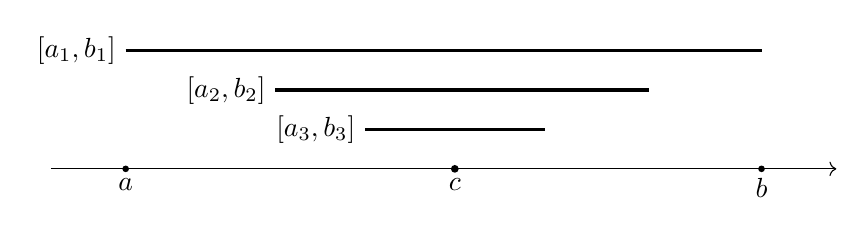
\begin{tikzpicture}[x=9.5cm,y=2.5cm]
  \draw[->] (0,0) -- (1.05,0);

  \coordinate (a) at (0.10,0);
  \coordinate (b) at (0.95,0);
  \fill (a) circle (1.2pt);
  \fill (b) circle (1.2pt);
  \node[below] at (a) {$a$};
  \node[below] at (b) {$b$};

  % nested intervals
  % 修改2：拉大 y 坐标的数值间隔 (0.6, 0.4, 0.2)
  \draw[very thick] (0.10,0.6) -- (0.95,0.6);
  \draw[very thick] (0.30,0.4) -- (0.80,0.4);
  \draw[very thick] (0.42,0.2) -- (0.66,0.2);

  % 修改3：将标签移到每条线段的起始位置左侧 (at 0.10, at 0.30...)
  % 这样标签呈阶梯状排列，完全避免重叠
  \node[left] at (0.10,0.6) {$[a_1,b_1]$};
  \node[left] at (0.30,0.4) {$[a_2,b_2]$};
  \node[left] at (0.42,0.2) {$[a_3,b_3]$};

  \coordinate (c) at (0.54,0);
  \fill (c) circle (1.4pt);
  \node[below] at (c) {$c$};
\end{tikzpicture}
\caption{Bisection produces nested intervals shrinking to a unique root location.}
\end{figure}

\begin{exercise}
Apply the bisection method to $f(x)=x^3-2$ on $[1,2]$ to produce an explicit $n$ such that the interval length is $<10^{-4}$.
Explain why this yields an approximation to $\sqrt[3]{2}$.
\end{exercise}

\newpage

% =========================
% Differentiation
% =========================

\section{Differentiation}

\begin{keyidea}
Differentiation formalizes the best linear approximation of a function near a point.
The derivative $f'(a)$, when it exists, is the unique real number such that
\[
f(a+h)=f(a)+f'(a)\,h + o(h)\quad (h\to 0).
\]
In this chapter we develop:
\begin{itemize}
\item the definition and basic rules of derivatives,
\item the Mean Value Theorem and its consequences,
\item Taylor's theorem (with a rigorous remainder),
\item qualitative behavior of functions via derivatives.
\end{itemize}
\end{keyidea}

% -------------------------------------------------
\subsection{Derivative and Basic Rules}

\subsubsection{Definition of the Derivative}

\begin{definition}[Derivative at a point]\label{def:derivative}
Let $f:D\to\RR$ with $D\subseteq\RR$, and let $a\in D$ be a point such that $a$ is a limit point of $D$
(i.e.\ there exist points of $D$ arbitrarily close to $a$).
We say that $f$ is \emph{differentiable at $a$} if the limit
\[
f'(a)\coloneqq \lim_{x\to a,\ x\in D,\ x\neq a}\frac{f(x)-f(a)}{x-a}
\]
exists in $\RR$. Equivalently, using $h=x-a$,
\[
f'(a)=\lim_{h\to 0,\ a+h\in D}\frac{f(a+h)-f(a)}{h}.
\]
\end{definition}

\begin{remark}
Differentiability is strictly stronger than continuity.
Indeed, if $f'(a)$ exists then $f$ must be continuous at $a$ (proved below).
\end{remark}

\begin{definition}[Differentiability on an interval]
If $I\subseteq\RR$ is an interval and $f:I\to\RR$, we say $f$ is \emph{differentiable on $I$}
if it is differentiable at every interior point of $I$.
At endpoints, one can define one-sided derivatives (useful later), but the classical Mean Value Theorem uses interior derivatives.
\end{definition}

\subsubsection{Geometric Meaning}

\begin{figure}[H]
\centering
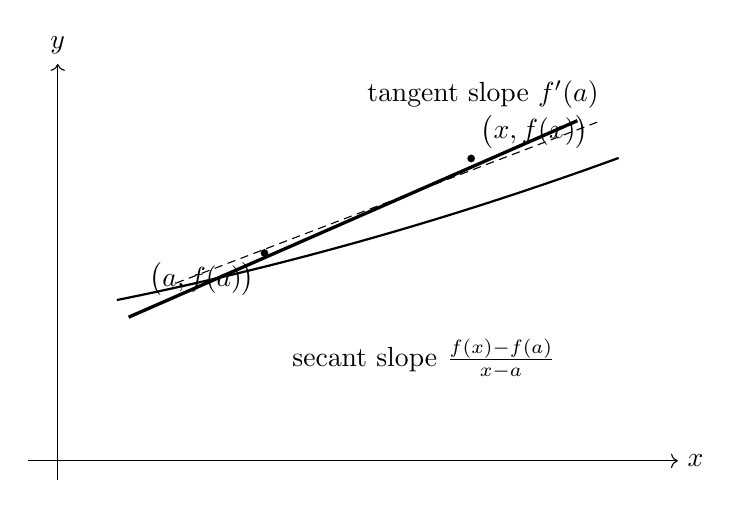
\begin{tikzpicture}[x=7.5cm,y=4.8cm]
  \draw[->] (-0.05,0) -- (1.05,0) node[right] {$x$};
  \draw[->] (0,-0.05) -- (0,1.05) node[above] {$y$};

  % a point a and nearby x
  \coordinate (A) at (0.35,0.55);
  \coordinate (X) at (0.70,0.80);

  % curve (stylized)
  \draw[thick,domain=0.10:0.95,samples=120]
    plot (\x,{0.35+0.45*\x+0.15*(\x-0.55)^2});

  % secant line
  \draw[densely dashed] (0.20,0.47) -- (0.92,0.90);

  % tangent line approximation at A (hand-tuned slope)
  \draw[very thick] (0.12,0.38) -- (0.88,0.90);

  \fill (A) circle (1.4pt);
  \fill (X) circle (1.4pt);

  \node[below left] at (A) {$\bigl(a,f(a)\bigr)$};
  \node[above right] at (X) {$\bigl(x,f(x)\bigr)$};

  \node at (0.62,0.27) {secant slope $\frac{f(x)-f(a)}{x-a}$};
  \node at (0.72,0.97) {tangent slope $f'(a)$};
\end{tikzpicture}
\caption{The derivative is the limiting slope of secant lines as $x\to a$.}
\end{figure}

\subsubsection{Differentiability Implies Continuity}

\begin{theorem}[Differentiability $\Rightarrow$ continuity]\label{thm:diff-implies-cont}
If $f$ is differentiable at $a$, then $f$ is continuous at $a$.
\end{theorem}

\begin{proof}
Assume $f'(a)$ exists. For $x\neq a$ (with $x\in D$),
\[
f(x)-f(a) = \frac{f(x)-f(a)}{x-a}\,(x-a).
\]
Take the limit as $x\to a$.
The difference quotient tends to $f'(a)$ by differentiability, and $(x-a)\to 0$.
By limit laws,
\[
\lim_{x\to a}\bigl(f(x)-f(a)\bigr) = f'(a)\cdot 0 = 0,
\]
so $f(x)\to f(a)$, i.e.\ $f$ is continuous at $a$.
\end{proof}

\subsubsection{Linearity and Product/Quotient Rules}

\begin{theorem}[Basic derivative rules]\label{thm:basic-deriv-rules}
Let $f,g:D\to\RR$ be differentiable at $a\in D$.
Then:
\begin{enumerate}[label=(\alph*)]
\item $(f+g)'(a)=f'(a)+g'(a)$.
\item For $c\in\RR$, $(cf)'(a)=c f'(a)$.
\item $(fg)'(a)=f'(a)g(a)+f(a)g'(a)$.
\item If $g(a)\neq 0$, then $(f/g)'(a)=\dfrac{f'(a)g(a)-f(a)g'(a)}{g(a)^2}$.
\end{enumerate}
\end{theorem}

\begin{proof}
(a) Using the definition,
\[
\frac{(f+g)(a+h)-(f+g)(a)}{h}
=
\frac{f(a+h)-f(a)}{h}+\frac{g(a+h)-g(a)}{h}.
\]
Taking $h\to 0$ gives $f'(a)+g'(a)$.

(b) Immediate from
\[
\frac{(cf)(a+h)-(cf)(a)}{h}=c\frac{f(a+h)-f(a)}{h}.
\]

(c) Compute
\begin{align*}
\frac{f(a+h)g(a+h)-f(a)g(a)}{h}
&=\frac{f(a+h)g(a+h)-f(a)g(a+h)}{h}
 +\frac{f(a)g(a+h)-f(a)g(a)}{h}\\
&=g(a+h)\frac{f(a+h)-f(a)}{h}+f(a)\frac{g(a+h)-g(a)}{h}.
\end{align*}
As $h\to 0$, $g(a+h)\to g(a)$ by continuity of $g$ (from \Cref{thm:diff-implies-cont}),
and the difference quotients tend to $f'(a)$ and $g'(a)$.
Thus the limit is $g(a)f'(a)+f(a)g'(a)$.

(d) First note that $g(a)\neq 0$ and continuity of $g$ imply $g(a+h)\neq 0$ for all sufficiently small $h$.
Then apply (c) to $f\cdot (1/g)$ once we show $(1/g)'(a)=-g'(a)/g(a)^2$.
Compute:
\[
\frac{\frac{1}{g(a+h)}-\frac{1}{g(a)}}{h}
=
\frac{g(a)-g(a+h)}{h\,g(a+h)\,g(a)}
=
-\frac{1}{g(a+h)g(a)}\cdot \frac{g(a+h)-g(a)}{h}.
\]
Let $h\to 0$. The factor $1/(g(a+h)g(a))\to 1/g(a)^2$, and the last quotient $\to g'(a)$,
giving $(1/g)'(a)=-g'(a)/g(a)^2$.
Then
\[
\left(\frac{f}{g}\right)'(a)=(f\cdot (1/g))'(a)=f'(a)\frac{1}{g(a)}+f(a)\left(-\frac{g'(a)}{g(a)^2}\right)
=\frac{f'(a)g(a)-f(a)g'(a)}{g(a)^2}.
\]
\end{proof}

\subsubsection{Chain Rule}

\begin{theorem}[Chain rule]\label{thm:chain-rule}
Let $f:D\to\RR$ be differentiable at $a\in D$, and let $g:E\to\RR$ be differentiable at $f(a)$, where $f(D)\subseteq E$.
Then $g\circ f$ is differentiable at $a$ and
\[
(g\circ f)'(a)=g'(f(a))\,f'(a).
\]
\end{theorem}

\begin{proof}
Let $h\to 0$ with $a+h\in D$ and define $\Delta f = f(a+h)-f(a)$.
Then
\[
\frac{g(f(a+h))-g(f(a))}{h}
=
\frac{g(f(a)+\Delta f)-g(f(a))}{\Delta f}\cdot \frac{\Delta f}{h},
\]
provided $\Delta f\neq 0$.
If $\Delta f=0$ along some sequence $h_k\to 0$, then the expression is $0$ along that subsequence, and the desired limit still holds
because $\Delta f/h \to f'(a)$ and $g'(f(a))$ is finite; we may proceed with the standard argument below which covers all cases.

Since $f$ is differentiable at $a$, we have $\Delta f\to 0$ and $\frac{\Delta f}{h}\to f'(a)$.
Since $g$ is differentiable at $f(a)$, we have
\[
\lim_{\Delta f\to 0}\frac{g(f(a)+\Delta f)-g(f(a))}{\Delta f}=g'(f(a)).
\]
Thus the product tends to $g'(f(a))\,f'(a)$ by limit laws.
\end{proof}

\subsubsection{Standard Derivatives (From First Principles)}

\begin{proposition}[Derivative of $x^n$ for $n\in\NN$]\label{prop:deriv-power}
For $n\in\NN$, the function $f(x)=x^n$ is differentiable on $\RR$ and
\[
\frac{d}{dx}x^n = n x^{n-1}.
\]
\end{proposition}

\begin{proof}
Fix $a\in\RR$.
Using the factorization $x^n-a^n=(x-a)\sum_{k=0}^{n-1}x^{n-1-k}a^k$ (valid for all real $x,a$),
for $x\neq a$ we have
\[
\frac{x^n-a^n}{x-a} = \sum_{k=0}^{n-1} x^{n-1-k}a^k.
\]
Let $x\to a$. Each term $x^{n-1-k}a^k \to a^{n-1-k}a^k=a^{n-1}$, and there are $n$ terms.
Hence the limit is $n a^{n-1}$, i.e.\ $f'(a)=n a^{n-1}$.
\end{proof}

\begin{corollary}
Every polynomial is differentiable on $\RR$ and its derivative is obtained by term-by-term differentiation.
Every rational function is differentiable on its domain.
\end{corollary}

\begin{exercise}
Prove from the definition that $\frac{d}{dx}\abs{x}$ does not exist at $x=0$.
(Hint: compute the difference quotient along $h>0$ and $h<0$.)
\end{exercise}

\newpage

% -------------------------------------------------
\subsection{Mean Value Theorem and Consequences}

\subsubsection{Rolle's Theorem}

\begin{theorem}[Rolle's theorem]\label{thm:rolle}
Let $f:[a,b]\to\RR$ be continuous on $[a,b]$ and differentiable on $(a,b)$.
If $f(a)=f(b)$, then there exists $c\in(a,b)$ such that $f'(c)=0$.
\end{theorem}

\begin{proof}
By the Extreme Value Theorem, $f$ attains a maximum and a minimum on $[a,b]$.
Let $x_{\max}$ be a point where the maximum is attained.
If $f$ is constant on $[a,b]$, then $f'(x)=0$ for all $x\in(a,b)$ and we are done.
Otherwise, the maximum value is strictly larger than the minimum value.
Since $f(a)=f(b)$, at least one of the extrema must occur at an interior point (otherwise both max and min would be at endpoints, forcing constancy).
Thus we can choose an interior extremum point $c\in(a,b)$ where either a maximum or a minimum occurs.

At such an interior extremum, we claim $f'(c)=0$.
For $h$ small with $c+h\in(a,b)$,
\[
\frac{f(c+h)-f(c)}{h}\le 0 \quad \text{for } h>0
\qquad\text{and}\qquad
\frac{f(c+h)-f(c)}{h}\ge 0 \quad \text{for } h<0
\]
if $c$ is a maximum (the inequalities reverse for a minimum, but the conclusion is the same).
Taking limits $h\to 0^\pm$ yields $f'(c)\le 0$ and $f'(c)\ge 0$, hence $f'(c)=0$.
\end{proof}

\subsubsection{Mean Value Theorem}

\begin{theorem}[Mean Value Theorem]\label{thm:mvt}
Let $f:[a,b]\to\RR$ be continuous on $[a,b]$ and differentiable on $(a,b)$.
Then there exists $c\in(a,b)$ such that
\[
f'(c)=\frac{f(b)-f(a)}{b-a}.
\]
\end{theorem}

\begin{proof}
Define the secant line
\[
\ell(x)\coloneqq f(a)+\frac{f(b)-f(a)}{b-a}(x-a),
\]
and consider $g(x)=f(x)-\ell(x)$.
Then $g$ is continuous on $[a,b]$ and differentiable on $(a,b)$, and
\[
g(a)=f(a)-\ell(a)=0,\qquad g(b)=f(b)-\ell(b)=0.
\]
By Rolle's theorem (\Cref{thm:rolle}), there exists $c\in(a,b)$ such that $g'(c)=0$.
But
\[
g'(x)=f'(x)-\frac{f(b)-f(a)}{b-a},
\]
so $g'(c)=0$ implies the desired identity.
\end{proof}

\subsubsection{Consequences: Monotonicity and Constant Functions}

\begin{theorem}[Derivative sign and monotonicity]\label{thm:monotone-deriv}
Let $f:(a,b)\to\RR$ be differentiable.
\begin{enumerate}[label=(\alph*)]
\item If $f'(x)\ge 0$ for all $x\in(a,b)$, then $f$ is nondecreasing on $(a,b)$.
\item If $f'(x)>0$ for all $x\in(a,b)$, then $f$ is strictly increasing on $(a,b)$.
\item If $f'(x)\le 0$ for all $x\in(a,b)$, then $f$ is nonincreasing on $(a,b)$.
\item If $f'(x)=0$ for all $x\in(a,b)$, then $f$ is constant on $(a,b)$.
\end{enumerate}
\end{theorem}

\begin{proof}
We prove (a) and (d); (b) and (c) are analogous.

(a) Take $x_1<x_2$ in $(a,b)$.
Apply the Mean Value Theorem to $f$ on $[x_1,x_2]$ to find $c\in(x_1,x_2)$ such that
\[
f(x_2)-f(x_1)=f'(c)(x_2-x_1).
\]
Since $x_2-x_1>0$ and $f'(c)\ge 0$, we have $f(x_2)\ge f(x_1)$, so $f$ is nondecreasing.

(d) If $f'(x)=0$ for all $x$, then by (a) $f$ is nondecreasing and by (c) $f$ is nonincreasing, hence constant.
Equivalently, apply MVT: for any $x_1<x_2$,
\[
f(x_2)-f(x_1)=f'(c)(x_2-x_1)=0,
\]
so $f(x_2)=f(x_1)$.
\end{proof}

\subsubsection{Uniqueness of Antiderivatives (Preview)}

\begin{corollary}[Antiderivatives differ by constants]\label{cor:antideriv-const}
Let $F,G:(a,b)\to\RR$ be differentiable and suppose $F'(x)=G'(x)$ for all $x\in(a,b)$.
Then $F-G$ is constant on $(a,b)$.
\end{corollary}

\begin{proof}
$(F-G)'=F'-G'=0$ on $(a,b)$. Apply \Cref{thm:monotone-deriv}(d).
\end{proof}

\subsubsection{Lipschitz Estimates}

\begin{theorem}[Bounded derivative implies Lipschitz]\label{thm:lipschitz}
Let $f:[a,b]\to\RR$ be continuous on $[a,b]$ and differentiable on $(a,b)$.
If $\abs{f'(x)}\le M$ for all $x\in(a,b)$, then for all $x,y\in[a,b]$,
\[
\abs{f(x)-f(y)}\le M\abs{x-y}.
\]
\end{theorem}

\begin{proof}
If $x=y$ there is nothing to show. Assume $x<y$.
Apply the Mean Value Theorem on $[x,y]$ to get $c\in(x,y)$ with
\[
f(y)-f(x)=f'(c)(y-x).
\]
Taking absolute values and using $\abs{f'(c)}\le M$ yields $\abs{f(y)-f(x)}\le M(y-x)=M\abs{x-y}$.
\end{proof}

\begin{remark}
This is stronger than uniform continuity: a Lipschitz function has a global linear modulus of continuity.
\end{remark}

\begin{exercise}
Let $f:[0,1]\to\RR$ be differentiable on $(0,1)$ and continuous on $[0,1]$.
If $f'(x)=0$ for all $x\in(0,1)$, show $f$ is constant on $[0,1]$.
Be explicit about how endpoints are handled.
\end{exercise}

\newpage

% -------------------------------------------------
\subsection{Inverse Function Theorem on the Real Line}

\subsubsection{Local Invertibility from a Nonzero Derivative}

\begin{theorem}[Inverse function theorem in $\RR$]\label{thm:ift-R}
Let $f:(a,b)\to\RR$ be differentiable and let $x_0\in(a,b)$ with $f'(x_0)\neq 0$.
Then there exists an open interval $I$ containing $x_0$ such that:
\begin{enumerate}[label=(\alph*)]
\item $f$ is strictly monotone on $I$, hence one-to-one on $I$;
\item $f(I)$ is an open interval;
\item the inverse function $f^{-1}:f(I)\to I$ is differentiable at $y_0=f(x_0)$ and
\[
(f^{-1})'(y_0)=\frac{1}{f'(x_0)}.
\]
\end{enumerate}
\end{theorem}

\begin{proof}
Assume $f'(x_0)>0$ (the case $f'(x_0)<0$ is similar with inequalities reversed).
By the definition of derivative,
\[
\lim_{x\to x_0}\frac{f(x)-f(x_0)}{x-x_0}=f'(x_0)>0.
\]
Hence there exists $\delta>0$ such that for all $x\in(x_0-\delta,x_0+\delta)$ with $x\neq x_0$,
\[
\frac{f(x)-f(x_0)}{x-x_0}>\frac{f'(x_0)}{2}>0.
\]
This implies:
\begin{itemize}
\item if $x>x_0$ then $f(x)>f(x_0)$,
\item if $x<x_0$ then $f(x)<f(x_0)$.
\end{itemize}
So $f$ is strictly increasing on $I=(x_0-\delta,x_0+\delta)$, hence one-to-one there.
Since $f$ is continuous on $I$, the image $f(I)$ is an interval, and because $f$ is strictly monotone it is in fact open (a standard argument using intermediate values; details omitted here but can be proved carefully).
Let $y_0=f(x_0)$.

Now consider the inverse $g=f^{-1}$ defined on $f(I)$.
To compute $g'(y_0)$, take $y\to y_0$ with $y\in f(I)$ and set $x=g(y)\in I$.
Then $x\to x_0$ and
\[
\frac{g(y)-g(y_0)}{y-y_0}=\frac{x-x_0}{f(x)-f(x_0)}.
\]
Taking $x\to x_0$ gives
\[
\lim_{y\to y_0}\frac{g(y)-g(y_0)}{y-y_0}
=
\left(\lim_{x\to x_0}\frac{f(x)-f(x_0)}{x-x_0}\right)^{-1}
=\frac{1}{f'(x_0)}.
\]
Thus $g$ is differentiable at $y_0$ with derivative $1/f'(x_0)$.
\end{proof}

\begin{remark}
This is the one-dimensional version of the Inverse Function Theorem.
In higher dimensions, the condition is invertibility of the Jacobian matrix.
\end{remark}

\begin{exercise}
Let $f(x)=x^3$. Use \Cref{thm:ift-R} to justify that $f^{-1}(y)=\sqrt[3]{y}$ is differentiable for all $y$ and compute $(f^{-1})'(y)$.
\end{exercise}

\newpage

% -------------------------------------------------
\subsection{Taylor's Theorem (One Variable)}

\subsubsection{Statement and Remainder}

\begin{definition}[Taylor polynomial]
Let $n\in\NN_0$ and suppose $f$ has derivatives up to order $n$ at $a$.
The \emph{Taylor polynomial of order $n$ at $a$} is
\[
T_n(x)=\sum_{k=0}^{n}\frac{f^{(k)}(a)}{k!}(x-a)^k.
\]
\end{definition}

\begin{theorem}[Taylor's theorem with Lagrange remainder]\label{thm:taylor}
Let $f:[a,b]\to\RR$ be such that $f^{(n+1)}$ exists on $(a,b)$ and extends continuously to $[a,b]$.
Then for each $x\in[a,b]$ there exists $\xi$ between $a$ and $x$ such that
\[
f(x)=T_n(x)+R_{n+1}(x),
\qquad
R_{n+1}(x)=\frac{f^{(n+1)}(\xi)}{(n+1)!}(x-a)^{n+1}.
\]
\end{theorem}

\begin{proof}
Fix $x\in[a,b]$, $x\neq a$ (the case $x=a$ is trivial).
Define the auxiliary function
\[
\Phi(t) \coloneqq f(t)-T_n(t)-\lambda (t-a)^{n+1},
\]
where $\lambda$ is chosen so that $\Phi(x)=0$.
Explicitly,
\[
\lambda \coloneqq \frac{f(x)-T_n(x)}{(x-a)^{n+1}}.
\]
By construction, $\Phi(a)=0$ (because $T_n(a)=f(a)$ and $(a-a)^{n+1}=0$) and $\Phi(x)=0$.

Moreover, $\Phi$ has derivatives up to order $n+1$ on $(a,b)$.
A direct computation shows that for $k=0,1,\dots,n$,
\[
\Phi^{(k)}(a)=0
\]
because $T_n$ matches the first $n$ derivatives of $f$ at $a$ and $(t-a)^{n+1}$ has a zero of order $n+1$ at $t=a$.

Now apply Rolle's theorem repeatedly:
Since $\Phi(a)=\Phi(x)=0$, there exists $c_1$ between $a$ and $x$ with $\Phi'(c_1)=0$.
Also $\Phi'(a)=0$ and $\Phi'(c_1)=0$, so there exists $c_2$ between $a$ and $c_1$ with $\Phi''(c_2)=0$.
Continuing in this way, we obtain a point $\xi$ between $a$ and $x$ such that
\[
\Phi^{(n+1)}(\xi)=0.
\]
But
\[
\Phi^{(n+1)}(t)=f^{(n+1)}(t)-\lambda (n+1)!,
\]
since $T_n$ has degree $n$ and its $(n+1)$st derivative is $0$, while $(t-a)^{n+1}$ differentiates to $(n+1)!$.
Thus $\Phi^{(n+1)}(\xi)=0$ implies
\[
\lambda=\frac{f^{(n+1)}(\xi)}{(n+1)!}.
\]
Substitute this into the definition of $\lambda$:
\[
\frac{f(x)-T_n(x)}{(x-a)^{n+1}}=\frac{f^{(n+1)}(\xi)}{(n+1)!},
\]
which rearranges to the stated remainder formula.
\end{proof}

\subsubsection{Error Bounds}

\begin{corollary}[Uniform bound on the remainder]\label{cor:taylor-bound}
Under the hypotheses of \Cref{thm:taylor}, if $\abs{f^{(n+1)}(t)}\le M$ for all $t\in[a,b]$, then for all $x\in[a,b]$,
\[
\abs{R_{n+1}(x)}\le \frac{M}{(n+1)!}\abs{x-a}^{n+1}.
\]
\end{corollary}

\begin{proof}
Use the remainder formula
\[
R_{n+1}(x)=\frac{f^{(n+1)}(\xi)}{(n+1)!}(x-a)^{n+1}
\]
for some $\xi$ between $a$ and $x$, then take absolute values and apply $\abs{f^{(n+1)}(\xi)}\le M$.
\end{proof}

\begin{exercise}
Assume $\abs{f''(t)}\le 10$ on $[-1,1]$ and $f(0)=0$, $f'(0)=2$.
Use Taylor's theorem with $n=1$ at $a=0$ to give a quantitative bound on $\abs{f(x)-2x}$ for $x\in[-1,1]$.
\end{exercise}

\newpage

% -------------------------------------------------
\subsection{Second Derivative and Shape}

\subsubsection{Local Extrema and the Second Derivative Test}

\begin{theorem}[Second derivative test]\label{thm:second-derivative}
Let $f$ be twice differentiable in a neighborhood of $a$ and assume $f'(a)=0$.
\begin{enumerate}[label=(\alph*)]
\item If $f''(a)>0$, then $f$ has a strict local minimum at $a$.
\item If $f''(a)<0$, then $f$ has a strict local maximum at $a$.
\item If $f''(a)=0$, no conclusion is possible in general.
\end{enumerate}
\end{theorem}

\begin{proof}
We prove (a). By Taylor's theorem of order $2$ at $a$, for $x$ near $a$ there exists $\xi$ between $a$ and $x$ such that
\[
f(x)=f(a)+f'(a)(x-a)+\frac{f''(\xi)}{2}(x-a)^2.
\]
Since $f'(a)=0$,
\[
f(x)-f(a)=\frac{f''(\xi)}{2}(x-a)^2.
\]
If $f''(a)>0$, continuity of $f''$ implies there exists a neighborhood of $a$ in which $f''(\xi)>0$.
Then for $x\neq a$ sufficiently close to $a$, we have $(x-a)^2>0$ and $f''(\xi)>0$, so $f(x)-f(a)>0$.
Hence $f(a)$ is a strict local minimum. The proof of (b) is analogous with signs reversed.
\end{proof}

\subsubsection{Convexity (Preview)}

\begin{definition}[Convex function]
A function $f:I\to\RR$ on an interval $I$ is \emph{convex} if for all $x,y\in I$ and all $\lambda\in[0,1]$,
\[
f(\lambda x+(1-\lambda)y)\le \lambda f(x)+(1-\lambda)f(y).
\]
\end{definition}

\begin{proposition}[Second derivative and convexity]\label{prop:convex-second}
If $f$ is twice differentiable on an interval $I$ and $f''(x)\ge 0$ for all $x\in I$, then $f$ is convex on $I$.
\end{proposition}

\begin{proof}
A standard proof uses the Mean Value Theorem on the derivative:
If $f''\ge 0$, then $f'$ is nondecreasing by \Cref{thm:monotone-deriv}.
This implies that secant slopes are increasing in their endpoints, which is equivalent to convexity.
(A complete derivation can be included once secant-slope characterization of convexity is established.)
\end{proof}

\begin{exercise}
Prove rigorously that if $f''\ge 0$ on $I$, then for $x<y<z$ in $I$,
\[
\frac{f(y)-f(x)}{y-x}\le \frac{f(z)-f(y)}{z-y}.
\]
Then deduce convexity from this inequality.
\end{exercise}

\newpage

% =========================
% The Riemann Integral
% =========================

\section{The Riemann Integral}

\begin{keyidea}
The Riemann integral is a precise way to define ``area under a curve'' for bounded functions on an interval.
Its core idea is approximation by rectangles:
\[
\int_a^b f(x)\,\diff x \approx \sum_{i=1}^n f(\xi_i)\,(x_i-x_{i-1}),
\]
where $a=x_0<\cdots<x_n=b$ is a partition and $\xi_i\in[x_{i-1},x_i]$ are sample points.
A function is Riemann integrable exactly when these approximations can be made arbitrarily accurate by refining the partition.
\end{keyidea}

% -------------------------------------------------
\subsection{Riemann Sums and Integrability}

\subsubsection{Partitions, Mesh, and Tagged Partitions}

\begin{definition}[Partition]\label{def:partition}
Let $a<b$. A \emph{partition} $P$ of $[a,b]$ is a finite set of points
\[
P=\{x_0,x_1,\dots,x_n\}\quad\text{with}\quad a=x_0<x_1<\cdots<x_n=b.
\]
We write $\Delta x_i \coloneqq x_i-x_{i-1}$ for the $i$th subinterval length.
The \emph{mesh} (or norm) of $P$ is
\[
\|P\|\coloneqq \max_{1\le i\le n}\Delta x_i.
\]
\end{definition}

\begin{definition}[Tagged partition and Riemann sum]\label{def:tagged}
A \emph{tagged partition} is a partition $P=\{x_0,\dots,x_n\}$ together with a choice of tags
\[
\xi_i\in[x_{i-1},x_i]\qquad (i=1,\dots,n).
\]
Given a bounded function $f:[a,b]\to\RR$, the \emph{Riemann sum} of $f$ with respect to $(P,\xi)$ is
\[
S(f,P,\xi)\coloneqq \sum_{i=1}^n f(\xi_i)\,\Delta x_i.
\]
\end{definition}

\begin{figure}[H]
\centering
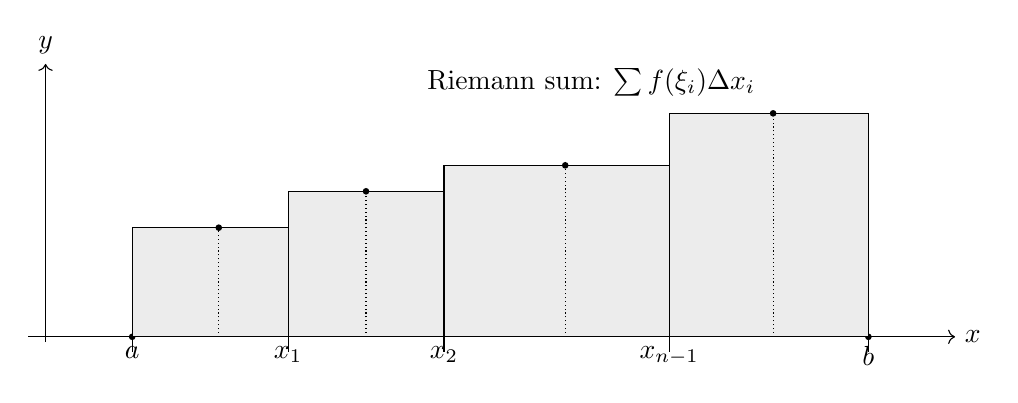
\begin{tikzpicture}[x=11cm,y=3.3cm]
  \draw[->] (-0.02,0) -- (1.05,0) node[right] {$x$};
  \draw[->] (0,-0.02) -- (0,1.05) node[above] {$y$};

  % interval endpoints
  \coordinate (a) at (0.10,0);
  \coordinate (b) at (0.95,0);
  \fill (a) circle (1.2pt);
  \fill (b) circle (1.2pt);
  \node[below] at (a) {$a$};
  \node[below] at (b) {$b$};

  % partition marks
  \foreach \xx/\lab in {0.10/a,0.28/x_1,0.46/x_2,0.72/x_{n-1},0.95/b}{
    \draw (\xx,0.06) -- (\xx,-0.06);
  }
  \node[below] at (0.28,0) {$x_1$};
  \node[below] at (0.46,0) {$x_2$};
  \node[below] at (0.72,0) {$x_{n-1}$};

  % simple "curve"
  \draw[thick,domain=0.10:0.95,samples=120]
    plot (\x,{0.25+0.55*(\x-0.10)+0.18*(\x-0.55)^2});

  % rectangles (schematic)
  \draw[fill=gray!15] (0.10,0) rectangle (0.28,0.42);
  \draw[fill=gray!15] (0.28,0) rectangle (0.46,0.56);
  \draw[fill=gray!15] (0.46,0) rectangle (0.72,0.66);
  \draw[fill=gray!15] (0.72,0) rectangle (0.95,0.86);

  % tags
  \foreach \xx/\yy in {0.20/0.42,0.37/0.56,0.60/0.66,0.84/0.86}{
    \fill (\xx,\yy) circle (1.2pt);
    \draw[densely dotted] (\xx,0) -- (\xx,\yy);
  }
  \node at (0.63,0.98) {Riemann sum: $\sum f(\xi_i)\Delta x_i$};
\end{tikzpicture}
\caption{A partition with sample points (tags) produces a rectangle approximation to the area.}
\end{figure}

\subsubsection{Upper and Lower Sums (Darboux Sums)}

\begin{definition}[Upper and lower sums]\label{def:upper-lower}
Let $f:[a,b]\to\RR$ be bounded and let $P=\{x_0,\dots,x_n\}$ be a partition.
For each subinterval $[x_{i-1},x_i]$, define
\[
M_i(f,P)\coloneqq \sup_{x\in[x_{i-1},x_i]} f(x),
\qquad
m_i(f,P)\coloneqq \inf_{x\in[x_{i-1},x_i]} f(x).
\]
The \emph{upper sum} and \emph{lower sum} are
\[
U(f,P)\coloneqq \sum_{i=1}^n M_i(f,P)\,\Delta x_i,
\qquad
L(f,P)\coloneqq \sum_{i=1}^n m_i(f,P)\,\Delta x_i.
\]
\end{definition}

\begin{proposition}[Refinement inequalities]\label{prop:refinement}
If $Q$ is a refinement of $P$ (i.e.\ $P\subseteq Q$), then
\[
L(f,P)\le L(f,Q)\le U(f,Q)\le U(f,P).
\]
\end{proposition}

\begin{proof}
Refining a partition splits some subintervals into smaller ones.
On a smaller interval the infimum can only increase and the supremum can only decrease, so the lower-sum terms weakly increase and the upper-sum terms weakly decrease.
Summing over subintervals gives the chain of inequalities.
\end{proof}

\begin{proposition}[Riemann sums sit between Darboux sums]\label{prop:between}
For any tagged partition $(P,\xi)$,
\[
L(f,P)\le S(f,P,\xi)\le U(f,P).
\]
\end{proposition}

\begin{proof}
Fix $i$. Since $\xi_i\in[x_{i-1},x_i]$, we have
\[
m_i(f,P)\le f(\xi_i)\le M_i(f,P).
\]
Multiply by $\Delta x_i\ge 0$ and sum from $i=1$ to $n$.
\end{proof}

\subsubsection{Darboux Integrability and the Definition of the Integral}

\begin{definition}[Upper/lower integrals]\label{def:upper-lower-integrals}
Let $f:[a,b]\to\RR$ be bounded.
Define the \emph{upper integral} and \emph{lower integral} by
\[
\overline{\int_a^b} f \coloneqq \inf_{P} U(f,P),
\qquad
\underline{\int_a^b} f \coloneqq \sup_{P} L(f,P),
\]
where the infimum/supremum range over all partitions of $[a,b]$.
\end{definition}

\begin{proposition}\label{prop:lower-le-upper}
For every bounded $f:[a,b]\to\RR$,
\[
\underline{\int_a^b} f \ \le\ \overline{\int_a^b} f.
\]
\end{proposition}

\begin{proof}
For any partition $P$, we have $L(f,P)\le U(f,P)$.
Taking the supremum over $P$ on the left and the infimum over $P$ on the right preserves the inequality.
\end{proof}

\begin{definition}[Riemann (Darboux) integrability]\label{def:riemann-int}
A bounded function $f:[a,b]\to\RR$ is \emph{Riemann integrable} if
\[
\underline{\int_a^b} f \ =\ \overline{\int_a^b} f.
\]
In this case the common value is denoted
\[
\int_a^b f(x)\,\diff x
\]
and is called the \emph{Riemann integral} of $f$ over $[a,b]$.
\end{definition}

\begin{theorem}[Characterization by upper--lower sums]\label{thm:UL-char}
A bounded function $f:[a,b]\to\RR$ is Riemann integrable if and only if
\[
\forall \eps>0\ \exists \text{ a partition }P \text{ such that } U(f,P)-L(f,P)<\eps.
\]
\end{theorem}

\begin{proof}
($\Rightarrow$) If $f$ is integrable, then
\[
\inf_P U(f,P)=\sup_P L(f,P)=I.
\]
Choose $P_1$ with $U(f,P_1)<I+\eps/2$ and $P_2$ with $L(f,P_2)>I-\eps/2$.
Let $P$ be a common refinement of $P_1$ and $P_2$ (take the union of their points).
Then by \Cref{prop:refinement},
\[
U(f,P)\le U(f,P_1)<I+\frac{\eps}{2},
\qquad
L(f,P)\ge L(f,P_2)>I-\frac{\eps}{2},
\]
hence $U(f,P)-L(f,P)<\eps$.

($\Leftarrow$) Assume the $\eps$-partition condition holds.
Let $I^-=\sup_P L(f,P)$ and $I^+=\inf_P U(f,P)$.
For any $\eps>0$ choose $P$ with $U(f,P)-L(f,P)<\eps$.
Then
\[
I^+ \le U(f,P) < L(f,P)+\eps \le I^-+\eps.
\]
Since always $I^-\le I^+$ by \Cref{prop:lower-le-upper}, we get
\[
0\le I^+-I^-<\eps.
\]
As $\eps>0$ is arbitrary, $I^+=I^-$, so $f$ is integrable.
\end{proof}

\subsubsection{Equivalence with the ``Riemann Sum'' Definition}

\begin{theorem}[Riemann sums characterize the integral]\label{thm:riemann-sums}
Let $f:[a,b]\to\RR$ be bounded and let $I\in\RR$.
Then the following are equivalent:
\begin{enumerate}[label=(\alph*)]
\item $f$ is Riemann integrable and $\displaystyle \int_a^b f(x)\,\diff x = I$.
\item For every $\eps>0$ there exists $\delta>0$ such that for every tagged partition $(P,\xi)$ with $\|P\|<\delta$,
\[
\abs{S(f,P,\xi)-I}<\eps.
\]
\end{enumerate}
\end{theorem}

\begin{proof}
We use the Darboux framework.

(a)$\Rightarrow$(b):
Let $I=\int_a^b f$ and fix $\eps>0$.
By \Cref{thm:UL-char}, choose a partition $P_0$ with
\[
U(f,P_0)-L(f,P_0)<\eps.
\]
Now take any tagged partition $(P,\xi)$ (no restriction on mesh is needed, but we proceed systematically) and form the common refinement
\[
Q \coloneqq P\cup P_0.
\]
By \Cref{prop:refinement} and \Cref{prop:between},
\[
L(f,Q)\le S(f,P,\xi)\le U(f,Q),
\qquad
L(f,P_0)\le L(f,Q)\le U(f,Q)\le U(f,P_0).
\]
Also, by definition of $I$ as both a supremum of lower sums and an infimum of upper sums,
\[
L(f,Q)\le I \le U(f,Q).
\]
Therefore,
\[
\abs{S(f,P,\xi)-I}
\le U(f,Q)-L(f,Q)
\le U(f,P_0)-L(f,P_0)
<\eps.
\]
Thus every Riemann sum is within $\eps$ of $I$; in particular the statement holds for any $\delta>0$.

(b)$\Rightarrow$(a):
Assume (b). Fix $\eps>0$ and choose $\delta>0$ such that $\|P\|<\delta$ implies $\abs{S(f,P,\xi)-I}<\eps/3$ for all tags.
Let $P$ be any partition with $\|P\|<\delta$.

For each subinterval $[x_{i-1},x_i]$, choose points $\xi_i,\eta_i\in[x_{i-1},x_i]$ such that
\[
f(\xi_i) > M_i(f,P) - \gamma,
\qquad
f(\eta_i) < m_i(f,P) + \gamma,
\]
where $\gamma>0$ will be specified momentarily.
(Such points exist because suprema/infima can be approximated arbitrarily well.)

Define the corresponding Riemann sums
\[
S^+ \coloneqq \sum_{i=1}^n f(\xi_i)\,\Delta x_i,
\qquad
S^- \coloneqq \sum_{i=1}^n f(\eta_i)\,\Delta x_i.
\]
Then
\[
U(f,P)-\gamma(b-a)\ \le\ S^+ \ \le\ U(f,P),
\qquad
L(f,P)\ \le\ S^- \ \le\ L(f,P)+\gamma(b-a).
\]
Choose $\gamma=\eps\bigl/3(b-a)$ (any positive choice with $\gamma(b-a)<\eps/3$ works).
Now (b) gives $\abs{S^+-I}<\eps/3$ and $\abs{S^--I}<\eps/3$.
Hence
\begin{align*}
U(f,P)-L(f,P)
&\le \bigl(U(f,P)-S^+\bigr)+\bigl(S^+-I\bigr)+\bigl(I-S^-\bigr)+\bigl(S^--L(f,P)\bigr)\\
&< \frac{\eps}{3}+\frac{\eps}{3}+\frac{\eps}{3}+\frac{\eps}{3}=\frac{4\eps}{3}.
\end{align*}
In particular, there exists a partition (namely this $P$) with $U(f,P)-L(f,P)<2\eps$.
Since $\eps>0$ was arbitrary, \Cref{thm:UL-char} implies $f$ is Riemann integrable.

Finally, to identify the integral with $I$, note that for integrable $f$ every Riemann sum can be made arbitrarily close to the integral,
so the only number satisfying (b) is the integral itself. Thus $\int_a^b f = I$.
\end{proof}

\subsubsection{Examples and Non-Examples}

\begin{example}[Constant and step functions]
If $f(x)=c$ on $[a,b]$, then every upper and lower sum equals $c(b-a)$, hence
\[
\int_a^b c\,\diff x = c(b-a).
\]
More generally, any step function (finite linear combination of indicator functions of intervals) is Riemann integrable.
\end{example}

\begin{example}[Dirichlet function is not Riemann integrable]\label{ex:dirichlet}
Define $f:[0,1]\to\RR$ by
\[
f(x)=
\casesm{
1, & x\in\QQ,\\
0, & x\in\RR\setminus\QQ.
}
\]
On every nontrivial interval, both rationals and irrationals occur, so on each subinterval $[x_{i-1},x_i]$ we have
\[
m_i(f,P)=0,\qquad M_i(f,P)=1.
\]
Hence for every partition $P$,
\[
L(f,P)=0,\qquad U(f,P)=1,
\]
so $\underline{\int_0^1} f=0$ and $\overline{\int_0^1} f=1$. Therefore $f$ is not Riemann integrable.
\end{example}

\begin{example}[Thomae's function is Riemann integrable with integral $0$]\label{ex:thomae}
Define $t:[0,1]\to\RR$ by
\[
t(0)=1,\qquad
t(x)=
\casesm{
\frac{1}{q}, & x=\frac{p}{q}\in(0,1]\ \text{in lowest terms},\\
0, & x\notin\QQ.
}
\]
Then $t$ is Riemann integrable on $[0,1]$ and
\[
\int_0^1 t(x)\,\diff x = 0.
\]

\smallskip
\noindent\emph{Sketch of a fully rigorous estimate.}
Fix $\eps>0$.
Choose $N\in\NN$ so that $1/N<\eps/2$.
Let
\[
A_N\coloneqq \left\{\frac{p}{q}\in[0,1]: 1\le q\le N,\ \gcd(p,q)=1\right\}.
\]
This set is finite. For each $r\in A_N$, choose an open interval $I_r$ around $r$ so small that the total length satisfies
\[
\sum_{r\in A_N} |I_r| < \frac{\eps}{2}.
\]
(We can do this because $A_N$ is finite.)
Now build a partition $P$ that includes all endpoints of the intervals $I_r$.

On subintervals lying outside $\bigcup_{r\in A_N} I_r$, any rational point has denominator $q>N$, hence $t(x)\le 1/N<\eps/2$,
and irrationals have value $0$.
Thus the supremum on those subintervals is at most $\eps/2$.

On subintervals contained in $\bigcup_{r\in A_N} I_r$, the supremum is at most $1$ (since $t(x)\le 1$ always).

Therefore the upper sum satisfies
\[
U(t,P)
\le
1\cdot \Bigl|\bigcup_{r\in A_N} I_r\Bigr|
\;+\;
\frac{\eps}{2}\cdot \Bigl(1-\Bigl|\bigcup_{r\in A_N} I_r\Bigr|\Bigr)
\le
\frac{\eps}{2}+\frac{\eps}{2}=\eps.
\]
Since $t\ge 0$, all lower sums are $\ge 0$, so $\underline{\int_0^1} t\ge 0$.
Letting $\eps\downarrow 0$ forces $\overline{\int_0^1} t=0$ and hence the integral is $0$.
\end{example}

\subsubsection{Continuous and Monotone Functions Are Integrable}

\begin{theorem}[Continuous functions are Riemann integrable]\label{thm:cont-int}
If $f:[a,b]\to\RR$ is continuous, then $f$ is Riemann integrable on $[a,b]$.
\end{theorem}

\begin{proof}
Since $[a,b]$ is compact, continuity implies uniform continuity.
Fix $\eps>0$.
Choose $\delta>0$ such that $\abs{x-y}<\delta$ implies
\[
\abs{f(x)-f(y)}<\frac{\eps}{b-a}.
\]
Let $P$ be any partition with $\|P\|<\delta$.
For each subinterval $[x_{i-1},x_i]$, the oscillation satisfies
\[
M_i(f,P)-m_i(f,P)\le \frac{\eps}{b-a}
\]
because any two points in the subinterval are within $\delta$ of each other.
Hence
\[
U(f,P)-L(f,P)
=\sum_{i=1}^n \bigl(M_i(f,P)-m_i(f,P)\bigr)\Delta x_i
\le \frac{\eps}{b-a}\sum_{i=1}^n \Delta x_i
=\frac{\eps}{b-a}(b-a)=\eps.
\]
By \Cref{thm:UL-char}, $f$ is Riemann integrable.
\end{proof}

\begin{theorem}[Monotone functions are Riemann integrable]\label{thm:mono-int}
If $f:[a,b]\to\RR$ is monotone (nondecreasing or nonincreasing), then $f$ is Riemann integrable on $[a,b]$.
\end{theorem}

\begin{proof}
Assume $f$ is nondecreasing (the other case is analogous).
Take an equal partition $P_n$ with $n$ subintervals:
\[
x_i=a+i\frac{b-a}{n}.
\]
On $[x_{i-1},x_i]$, we have
\[
m_i(f,P_n)=f(x_{i-1}),\qquad M_i(f,P_n)=f(x_i).
\]
Thus
\begin{align*}
U(f,P_n)-L(f,P_n)
&=\sum_{i=1}^n \bigl(f(x_i)-f(x_{i-1})\bigr)\Delta x_i\\
&=\frac{b-a}{n}\sum_{i=1}^n \bigl(f(x_i)-f(x_{i-1})\bigr)
=\frac{b-a}{n}\bigl(f(b)-f(a)\bigr).
\end{align*}
As $n\to\infty$ this tends to $0$, so for large $n$ it is $<\eps$.
By \Cref{thm:UL-char}, $f$ is integrable.
\end{proof}

\begin{exercise}
Let $f:[a,b]\to\RR$ be bounded. Prove that if $f$ is Riemann integrable and $g=f$ except at finitely many points, then $g$ is Riemann integrable and
\[
\int_a^b g(x)\,\diff x = \int_a^b f(x)\,\diff x.
\]
(Hint: isolate each exceptional point inside a tiny subinterval of total length $<\eps$.)
\end{exercise}

\newpage

% -------------------------------------------------
\subsection{Properties of the Riemann Integral}

\subsubsection{Linearity, Order, and Bounds}

\begin{theorem}[Linearity]\label{thm:int-linearity}
If $f,g$ are Riemann integrable on $[a,b]$ and $\alpha,\beta\in\RR$, then $\alpha f+\beta g$ is Riemann integrable and
\[
\int_a^b (\alpha f(x)+\beta g(x))\,\diff x
=
\alpha\int_a^b f(x)\,\diff x+\beta\int_a^b g(x)\,\diff x.
\]
\end{theorem}

\begin{proof}
Using upper/lower sums, one checks that for any partition $P$,
\[
U(\alpha f+\beta g,P)\le \alpha U(f,P)+\beta U(g,P)
\quad\text{and}\quad
L(\alpha f+\beta g,P)\ge \alpha L(f,P)+\beta L(g,P)
\]
when $\alpha,\beta\ge 0$, and extends to general scalars by decomposing into positive and negative parts.
Equivalently (and often more directly), use the Riemann sum characterization \Cref{thm:riemann-sums} and limit laws for sequences of sums.
\end{proof}

\begin{theorem}[Monotonicity]\label{thm:int-monotone}
If $f,g$ are integrable on $[a,b]$ and $f(x)\le g(x)$ for all $x\in[a,b]$, then
\[
\int_a^b f(x)\,\diff x \le \int_a^b g(x)\,\diff x.
\]
\end{theorem}

\begin{proof}
For any partition $P$, we have $m_i(f,P)\le m_i(g,P)$ and $M_i(f,P)\le M_i(g,P)$, hence
\[
L(f,P)\le L(g,P),\qquad U(f,P)\le U(g,P).
\]
Taking suprema/infima and using integrability yields the desired inequality.
\end{proof}

\begin{corollary}[Integral bounds from pointwise bounds]\label{cor:int-bounds}
If $f$ is integrable and $m\le f(x)\le M$ for all $x\in[a,b]$, then
\[
m(b-a)\le \int_a^b f(x)\,\diff x \le M(b-a).
\]
\end{corollary}

\begin{proof}
Apply \Cref{thm:int-monotone} to the constant functions $m$ and $M$ and use $\int_a^b c\,\diff x=c(b-a)$.
\end{proof}

\subsubsection{Additivity Over Intervals}

\begin{theorem}[Additivity]\label{thm:int-add}
Let $f$ be Riemann integrable on $[a,b]$ and let $c\in(a,b)$.
Then $f$ is integrable on $[a,c]$ and on $[c,b]$, and
\[
\int_a^b f(x)\,\diff x = \int_a^c f(x)\,\diff x + \int_c^b f(x)\,\diff x.
\]
\end{theorem}

\begin{proof}
Given a partition $P$ of $[a,b]$, refine it (if needed) so that $c$ is a partition point.
Then the upper and lower sums split exactly into sums over $[a,c]$ and $[c,b]$.
Using \Cref{thm:UL-char} on each subinterval (and conversely combining partitions) shows integrability and the identity of integrals.
\end{proof}

\subsubsection{Absolute Values and Continuous Transformations}

\begin{theorem}[Integrability is stable under continuous transforms]\label{thm:cont-transform}
Let $f$ be Riemann integrable on $[a,b]$.
Let $\varphi:\RR\to\RR$ be continuous.
Then $\varphi\circ f$ is Riemann integrable on $[a,b]$.
\end{theorem}

\begin{proof}
Since $f$ is integrable, it is bounded: $\abs{f(x)}\le M$ on $[a,b]$ for some $M$.
The restriction of $\varphi$ to the compact interval $[-M,M]$ is uniformly continuous.
Hence, for every $\eps>0$ there exists $\eta>0$ such that for all $u,v\in[-M,M]$,
\[
\abs{u-v}<\eta \ \Rightarrow\ \abs{\varphi(u)-\varphi(v)}<\frac{\eps}{b-a}.
\]
Because $f$ is integrable, there exists a partition $P$ such that on each subinterval the oscillation of $f$ is $<\eta$ in the sense that
\[
M_i(f,P)-m_i(f,P)<\eta \quad\text{for all }i
\]
(after refining enough; a standard consequence of \Cref{thm:UL-char}).
Then on each subinterval, the oscillation of $\varphi\circ f$ is $<\eps/(b-a)$.
Therefore,
\[
U(\varphi\circ f,P)-L(\varphi\circ f,P)
\le \frac{\eps}{b-a}\sum_{i=1}^n \Delta x_i
=\eps.
\]
By \Cref{thm:UL-char}, $\varphi\circ f$ is integrable.
\end{proof}

\begin{corollary}[Absolute value and triangle inequality]\label{cor:abs-int}
If $f$ is Riemann integrable on $[a,b]$, then $\abs{f}$ is Riemann integrable and
\[
\abs{\int_a^b f(x)\,\diff x}\le \int_a^b \abs{f(x)}\,\diff x.
\]
\end{corollary}

\begin{proof}
Integrability of $\abs{f}$ follows from \Cref{thm:cont-transform} with $\varphi(u)=\abs{u}$.
For the inequality, note that $-\abs{f}\le f\le \abs{f}$ pointwise, so by \Cref{thm:int-monotone},
\[
-\int_a^b \abs{f}\,\diff x \le \int_a^b f\,\diff x \le \int_a^b \abs{f}\,\diff x,
\]
which is equivalent to the stated estimate.
\end{proof}

\begin{corollary}[Products and quotients]\label{cor:prod-quot}
If $f$ and $g$ are Riemann integrable on $[a,b]$, then $fg$ is Riemann integrable.
If additionally $g(x)\neq 0$ for all $x$ and $1/g$ is bounded on $[a,b]$, then $f/g$ is Riemann integrable.
\end{corollary}

\begin{proof}
The map $(u,v)\mapsto uv$ is continuous on $\RR^2$; on bounded ranges one can reduce to a one-variable continuous transform using algebraic identities (or prove directly via oscillation estimates).
For the quotient, use $f/g=f\cdot (1/g)$ and continuity of $u\mapsto 1/u$ on any set bounded away from $0$.
\end{proof}

\subsubsection{Mean Value Theorem for Integrals}

\begin{theorem}[Mean value theorem for integrals]\label{thm:mvt-integral}
If $f:[a,b]\to\RR$ is continuous, then there exists $c\in[a,b]$ such that
\[
\int_a^b f(x)\,\diff x = f(c)\,(b-a).
\]
\end{theorem}

\begin{proof}
By the Extreme Value Theorem, $f$ attains a minimum $m$ and maximum $M$ on $[a,b]$.
Thus $m\le f(x)\le M$ for all $x$, so by \Cref{cor:int-bounds},
\[
m(b-a)\le \int_a^b f(x)\,\diff x \le M(b-a).
\]
Divide by $(b-a)>0$:
\[
m \le \frac{1}{b-a}\int_a^b f(x)\,\diff x \le M.
\]
Because $f([a,b])$ is an interval (continuous image of a connected set), every value between $m$ and $M$ is achieved.
Hence there exists $c$ with $f(c)=\frac{1}{b-a}\int_a^b f$.
\end{proof}

\begin{exercise}
Let $f$ be integrable on $[a,b]$ and define $F(x)=\int_a^x f(t)\,\diff t$.
Prove that $F$ is uniformly continuous on $[a,b]$.
(Hint: use \Cref{cor:int-bounds} with a bound on $\abs{f}$.)
\end{exercise}

\newpage

% -------------------------------------------------
\subsection{Fundamental Theorem of Calculus}

\subsubsection{The Integral Defines a Continuous Accumulation Function}

\begin{theorem}[Continuity of the accumulation function]\label{thm:accum-cont}
Let $f:[a,b]\to\RR$ be Riemann integrable, and define for $x\in[a,b]$,
\[
F(x)\coloneqq \int_a^x f(t)\,\diff t.
\]
Then $F$ is continuous on $[a,b]$.
Moreover, if $\abs{f(t)}\le M$ on $[a,b]$, then for all $x,y\in[a,b]$,
\[
\abs{F(x)-F(y)}\le M\abs{x-y}.
\]
\end{theorem}

\begin{proof}
Assume $x<y$ (the other case is symmetric).
By additivity (\Cref{thm:int-add}),
\[
F(y)-F(x)=\int_x^y f(t)\,\diff t.
\]
If $\abs{f(t)}\le M$, then $-M\le f(t)\le M$, so by \Cref{cor:int-bounds},
\[
-M(y-x)\le \int_x^y f(t)\,\diff t \le M(y-x).
\]
Thus $\abs{F(y)-F(x)}\le M\abs{y-x}$, which implies continuity (indeed Lipschitz continuity).
\end{proof}

\subsubsection{Fundamental Theorem of Calculus, Part I}

\begin{theorem}[FTC I: differentiation of the integral]\label{thm:ftc1}
Let $f:[a,b]\to\RR$ be Riemann integrable and define $F(x)=\int_a^x f(t)\,\diff t$.
If $f$ is continuous at a point $x_0\in(a,b)$, then $F$ is differentiable at $x_0$ and
\[
F'(x_0)=f(x_0).
\]
In particular, if $f$ is continuous on $[a,b]$, then $F$ is differentiable on $(a,b)$ with $F'=f$.
\end{theorem}

\begin{proof}
Fix $x_0\in(a,b)$ where $f$ is continuous.
For $h$ small enough that $x_0+h\in[a,b]$, we have
\[
\frac{F(x_0+h)-F(x_0)}{h}
=
\frac{1}{h}\int_{x_0}^{x_0+h} f(t)\,\diff t.
\]
Assume $h>0$ first. Let
\[
m(h)\coloneqq \inf_{t\in[x_0,x_0+h]} f(t),
\qquad
M(h)\coloneqq \sup_{t\in[x_0,x_0+h]} f(t).
\]
Then
\[
m(h)\,h \le \int_{x_0}^{x_0+h} f(t)\,\diff t \le M(h)\,h,
\]
so dividing by $h>0$ gives
\[
m(h)\le \frac{F(x_0+h)-F(x_0)}{h}\le M(h).
\]
Because $f$ is continuous at $x_0$, the oscillation on $[x_0,x_0+h]$ shrinks as $h\to 0^+$, and specifically
\[
m(h)\to f(x_0),\qquad M(h)\to f(x_0)\qquad (h\to 0^+).
\]
By the squeeze theorem,
\[
\lim_{h\to 0^+}\frac{F(x_0+h)-F(x_0)}{h}=f(x_0).
\]

For $h<0$, apply the same argument on $[x_0+h,x_0]$ and note that
\[
\frac{F(x_0+h)-F(x_0)}{h}
=
\frac{1}{h}\int_{x_0}^{x_0+h} f(t)\,\diff t
=
\frac{1}{h}\left(-\int_{x_0+h}^{x_0} f(t)\,\diff t\right),
\]
which again is squeezed between the infimum and supremum on the interval, leading to the same limit $f(x_0)$ as $h\to 0^-$.
Therefore the two-sided derivative exists and equals $f(x_0)$.
\end{proof}

\subsubsection{Fundamental Theorem of Calculus, Part II}

\begin{theorem}[FTC II: integrating a derivative]\label{thm:ftc2}
Let $F:[a,b]\to\RR$ be continuous on $[a,b]$ and differentiable on $(a,b)$.
Assume $F'$ is Riemann integrable on $[a,b]$.
Then
\[
\int_a^b F'(x)\,\diff x = F(b)-F(a).
\]
\end{theorem}

\begin{proof}
Let $P=\{x_0,\dots,x_n\}$ be any partition of $[a,b]$.
For each $i$, apply the Mean Value Theorem to $F$ on $[x_{i-1},x_i]$ to obtain $c_i\in(x_{i-1},x_i)$ such that
\[
F(x_i)-F(x_{i-1}) = F'(c_i)\,(x_i-x_{i-1})=F'(c_i)\,\Delta x_i.
\]
Summing over $i$ gives a telescoping sum:
\[
F(b)-F(a)=\sum_{i=1}^n F'(c_i)\,\Delta x_i.
\]
The right-hand side is precisely a Riemann sum $S(F',P,\xi)$ with tags $\xi_i=c_i$.
Since $F'$ is integrable, by \Cref{thm:riemann-sums} these Riemann sums converge to $\int_a^b F'(x)\,\diff x$ as $\|P\|\to 0$.
Therefore $F(b)-F(a)$ equals the integral of $F'$.
\end{proof}

\begin{remark}
The hypothesis ``$F'$ is integrable'' is automatic if $F'$ is continuous.
In many calculus settings, $F'$ is assumed continuous, and then FTC II follows immediately.
\end{remark}

\subsubsection{Change of Variables (Substitution)}

\begin{theorem}[Change of variables]\label{thm:substitution}
Let $\varphi:[\alpha,\beta]\to[a,b]$ be continuously differentiable and strictly monotone, with $\varphi(\alpha)=a$ and $\varphi(\beta)=b$.
Let $f:[a,b]\to\RR$ be continuous.
Then
\[
\int_a^b f(x)\,\diff x = \int_\alpha^\beta f(\varphi(t))\,\varphi'(t)\,\diff t.
\]
\end{theorem}

\begin{proof}
Let $F(x)\coloneqq \int_a^x f(u)\,\diff u$. By \Cref{thm:ftc1}, $F$ is differentiable with $F'(x)=f(x)$.
Consider the composition $H(t)\coloneqq F(\varphi(t))$.
By the chain rule,
\[
H'(t)=F'(\varphi(t))\,\varphi'(t)=f(\varphi(t))\,\varphi'(t).
\]
Integrate $H'$ over $[\alpha,\beta]$ and apply \Cref{thm:ftc2}:
\[
\int_\alpha^\beta f(\varphi(t))\,\varphi'(t)\,\diff t
=
\int_\alpha^\beta H'(t)\,\diff t
=
H(\beta)-H(\alpha)
=
F(b)-F(a)
=
\int_a^b f(x)\,\diff x.
\]
\end{proof}

\subsubsection{Integration by Parts}

\begin{theorem}[Integration by parts]\label{thm:ibp}
Let $u,v:[a,b]\to\RR$ be continuously differentiable.
Then
\[
\int_a^b u(x)\,v'(x)\,\diff x
=
u(b)v(b)-u(a)v(a) - \int_a^b u'(x)\,v(x)\,\diff x.
\]
\end{theorem}

\begin{proof}
By the product rule, $(uv)'=u'v+uv'$.
Integrate both sides and apply \Cref{thm:ftc2}:
\[
\int_a^b (u(x)v(x))'\,\diff x = u(b)v(b)-u(a)v(a)
=
\int_a^b u'(x)v(x)\,\diff x+\int_a^b u(x)v'(x)\,\diff x.
\]
Rearrange to obtain the formula.
\end{proof}

\subsubsection{A Visual: Upper/Lower Sums Converging to Area}

\begin{figure}[H]
\centering
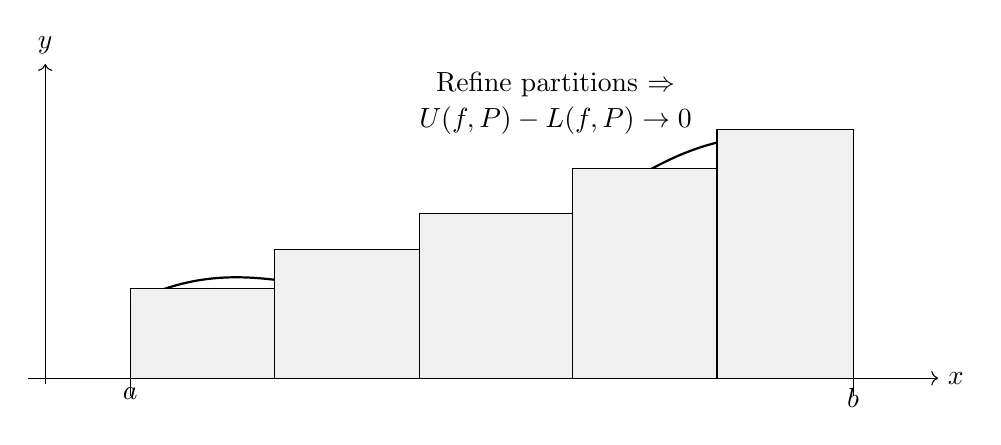
\begin{tikzpicture}[x=10.8cm,y=3.8cm]
  \draw[->] (-0.02,0) -- (1.05,0) node[right] {$x$};
  \draw[->] (0,-0.02) -- (0,1.05) node[above] {$y$};

  % curve
  \draw[thick,domain=0.10:0.95,samples=140]
    plot (\x,{0.15+0.75*(\x-0.10)+0.12*sin(10*\x r)});

  % axes labels for a,b
  \draw (0.10,0.06) -- (0.10,-0.06);
  \draw (0.95,0.06) -- (0.95,-0.06);
  \node[below] at (0.10,0) {$a$};
  \node[below] at (0.95,0) {$b$};

  % a few lower rectangles (schematic; heights chosen to avoid overlap)
  \draw[fill=gray!12] (0.10,0) rectangle (0.27,0.30);
  \draw[fill=gray!12] (0.27,0) rectangle (0.44,0.43);
  \draw[fill=gray!12] (0.44,0) rectangle (0.62,0.55);
  \draw[fill=gray!12] (0.62,0) rectangle (0.79,0.70);
  \draw[fill=gray!12] (0.79,0) rectangle (0.95,0.83);

  \node at (0.60,0.98) {Refine partitions $\Rightarrow$};
  \node at (0.60,0.86) {$U(f,P)-L(f,P)\to 0$};
\end{tikzpicture}
\caption{As partitions are refined, lower and upper rectangle approximations squeeze toward the true integral.}
\end{figure}

\subsubsection{Applications and Quick Computations (with Full Justification)}

\begin{example}[A classic consequence: $\int_a^b x^n\,\diff x$]
For $n\in\NN_0$, define $F(x)=\frac{x^{n+1}}{n+1}$.
Then $F'(x)=x^n$ is continuous, hence integrable, and by FTC II,
\[
\int_a^b x^n\,\diff x = F(b)-F(a)=\frac{b^{n+1}-a^{n+1}}{n+1}.
\]
\end{example}

\begin{example}[Substitution]
Let $f$ be continuous and compute $\int_0^1 2t\,f(t^2)\,\diff t$.
Set $\varphi(t)=t^2$, so $\varphi'(t)=2t$ and $\varphi([0,1])=[0,1]$.
By \Cref{thm:substitution},
\[
\int_0^1 2t\,f(t^2)\,\diff t
=\int_0^1 f(x)\,\diff x.
\]
\end{example}

\begin{example}[Integration by parts]
If $u,v$ are $C^1$, then
\[
\int_a^b x\,f'(x)\,\diff x
=
\bigl[x f(x)\bigr]_{a}^{b}-\int_a^b 1\cdot f(x)\,\diff x
=
b f(b)-a f(a)-\int_a^b f(x)\,\diff x.
\]
This is \Cref{thm:ibp} with $u(x)=x$ and $v(x)=f(x)$.
\end{example}

\begin{exercise}
Let $f:[a,b]\to\RR$ be continuous and define $F(x)=\int_a^x f$.
Show that $F$ is differentiable on $(a,b)$ and that $F$ is constant on $[a,b]$ if and only if $f\equiv 0$.
\end{exercise}

\begin{exercise}
Assume $f$ is continuous on $[a,b]$ and $\int_a^b f(x)\,\diff x=0$.
Is it necessarily true that $f(x)=0$ for all $x$?
If not, give a counterexample; if yes, state the additional hypotheses needed.
\end{exercise}

\begin{exercise}
Prove that if $f$ is integrable on $[a,b]$ and $f(x)\ge 0$ for all $x$, then $\int_a^b f=0$ implies:
for every $\eps>0$, the set $\{x\in[a,b]: f(x)\ge \eps\}$ can be covered by finitely many intervals of arbitrarily small total length.
(Interpretation: a nonnegative integrable function with zero integral must be ``small almost everywhere'' in a Riemann sense.)
\end{exercise}

\newpage

% =========================
% Sequences of Functions and Uniform Convergence
% =========================

\section{Sequences of Functions and Uniform Convergence}

\begin{keyidea}
For sequences of real numbers, convergence is about controlling a single tail.
For sequences of functions, there are \emph{two} variables: the index $n$ and the point $x$.
Uniform convergence is the correct notion when we want to pass limits through
\emph{continuous operations} such as continuity, integration, and differentiation.
\end{keyidea}

% -------------------------------------------------
\subsection{Pointwise vs.\ Uniform Convergence}

\subsubsection{Two Notions of Convergence}

\begin{definition}[Pointwise convergence]\label{def:pointwise}
Let $D\subseteq\RR$ and let $(f_n)$ be a sequence of functions $f_n:D\to\RR$.
We say $f_n\to f$ \emph{pointwise} on $D$ if for every $x\in D$,
\[
\lim_{n\to\infty} f_n(x)=f(x).
\]
Equivalently: for every $x\in D$ and every $\eps>0$, there exists $N=N(\eps,x)$ such that
$n\ge N \Rightarrow \abs{f_n(x)-f(x)}<\eps$.
\end{definition}

\begin{definition}[Uniform convergence]\label{def:uniform}
Let $D\subseteq\RR$ and $f_n,f:D\to\RR$.
We say $f_n\to f$ \emph{uniformly} on $D$ if
\[
\forall \eps>0\ \exists N=N(\eps)\ \forall n\ge N\ \forall x\in D,\quad
\abs{f_n(x)-f(x)}<\eps.
\]
The key difference from pointwise convergence is that $N$ depends on $\eps$ but \emph{not} on $x$.
\end{definition}

\begin{remark}
Uniform convergence is strictly stronger than pointwise convergence:
\[
f_n\to f \text{ uniformly } \ \Rightarrow\ f_n\to f \text{ pointwise}.
\]
The converse is false in general.
\end{remark}

\subsubsection{The Sup Norm Viewpoint}

\begin{definition}[Sup norm]\label{def:supnorm}
If $f:D\to\RR$ is bounded, define
\[
\|f\|_{\infty,D}\coloneqq \sup_{x\in D}\abs{f(x)}\in[0,\infty).
\]
When $D$ is clear, we write $\|f\|_\infty$.
\end{definition}

\begin{proposition}[Uniform convergence $\Leftrightarrow$ sup norm convergence]\label{prop:uniform-sup}
Assume $f_n-f$ is bounded on $D$ for all $n$.
Then
\[
f_n\to f \text{ uniformly on }D
\quad\Longleftrightarrow\quad
\|f_n-f\|_{\infty,D}\to 0.
\]
\end{proposition}

\begin{proof}
By definition,
\[
\|f_n-f\|_{\infty,D}=\sup_{x\in D}\abs{f_n(x)-f(x)}.
\]
The statement $\|f_n-f\|_{\infty,D}\to 0$ means:
for every $\eps>0$ there exists $N$ such that $n\ge N$ implies
$\sup_{x\in D}\abs{f_n(x)-f(x)}<\eps$, which is equivalent to
$\abs{f_n(x)-f(x)}<\eps$ for all $x\in D$.
This is exactly uniform convergence.
\end{proof}

\subsubsection{Uniform Cauchy Criterion}

\begin{definition}[Uniformly Cauchy]\label{def:uniform-cauchy}
A sequence $(f_n)$ on $D$ is \emph{uniformly Cauchy} if
\[
\forall \eps>0\ \exists N\ \forall m,n\ge N\ \forall x\in D,\quad
\abs{f_n(x)-f_m(x)}<\eps.
\]
Equivalently, $\|f_n-f_m\|_{\infty,D}\to 0$ as $m,n\to\infty$.
\end{definition}

\begin{theorem}[Completeness under uniform convergence]\label{thm:uniform-complete}
Let $D\subseteq\RR$. If $(f_n)$ is uniformly Cauchy on $D$, then there exists a function $f:D\to\RR$ such that
$f_n\to f$ uniformly on $D$.
\end{theorem}

\begin{proof}
Fix $x\in D$. The condition ``uniformly Cauchy'' implies in particular that $(f_n(x))$ is a Cauchy sequence in $\RR$:
for every $\eps>0$ there exists $N$ such that for $m,n\ge N$,
\[
\abs{f_n(x)-f_m(x)}<\eps.
\]
Since $\RR$ is complete, $(f_n(x))$ converges to some real number; define
\[
f(x)\coloneqq \lim_{n\to\infty} f_n(x).
\]
We claim $f_n\to f$ uniformly. Let $\eps>0$ and choose $N$ from the uniform Cauchy property so that
$\abs{f_n(x)-f_m(x)}<\eps$ for all $m,n\ge N$ and all $x\in D$.
Fix $n\ge N$ and $x\in D$. Let $m\to\infty$; then $f_m(x)\to f(x)$, and by taking limits in
$\abs{f_n(x)-f_m(x)}<\eps$, we obtain
\[
\abs{f_n(x)-f(x)}\le \eps.
\]
This holds for all $x\in D$, hence $\|f_n-f\|_{\infty,D}\le \eps$ for all $n\ge N$.
Therefore $f_n\to f$ uniformly on $D$.
\end{proof}

\subsubsection{A Canonical Example: Pointwise but Not Uniform}

\begin{example}[The sequence $x^n$ on {$[0,1]$}]\label{ex:xn}
Let $f_n:[0,1]\to\RR$ be $f_n(x)=x^n$.
Then $f_n\to f$ pointwise on $[0,1]$, where
\[
f(x)=
\casesm{
0, & 0\le x<1,\\
1, & x=1.
}
\]
However, $f_n$ does \emph{not} converge uniformly to $f$ on $[0,1]$.
\end{example}

\begin{proof}
\textbf{Pointwise convergence.}
Fix $x\in[0,1)$. Then $0\le x<1$, so $x^n\to 0$ as $n\to\infty$ (geometric decay).
At $x=1$, $f_n(1)=1$ for all $n$, so the limit is $1$.

\textbf{Failure of uniform convergence.}
Take $\eps=\tfrac12$.
For each $n$, choose
\[
x_n\coloneqq \left(\tfrac12\right)^{1/n}\in(0,1).
\]
Then $f(x_n)=0$ (since $x_n<1$) and
\[
\abs{f_n(x_n)-f(x_n)}=\abs{x_n^n-0}=\tfrac12.
\]
Thus for every $N$ we can take $n\ge N$ and find an $x=x_n$ with
$\abs{f_n(x)-f(x)}=\tfrac12\not<\tfrac12$.
So no single $N$ works for all $x$, and uniform convergence fails.
\end{proof}

\begin{figure}[H]
\centering
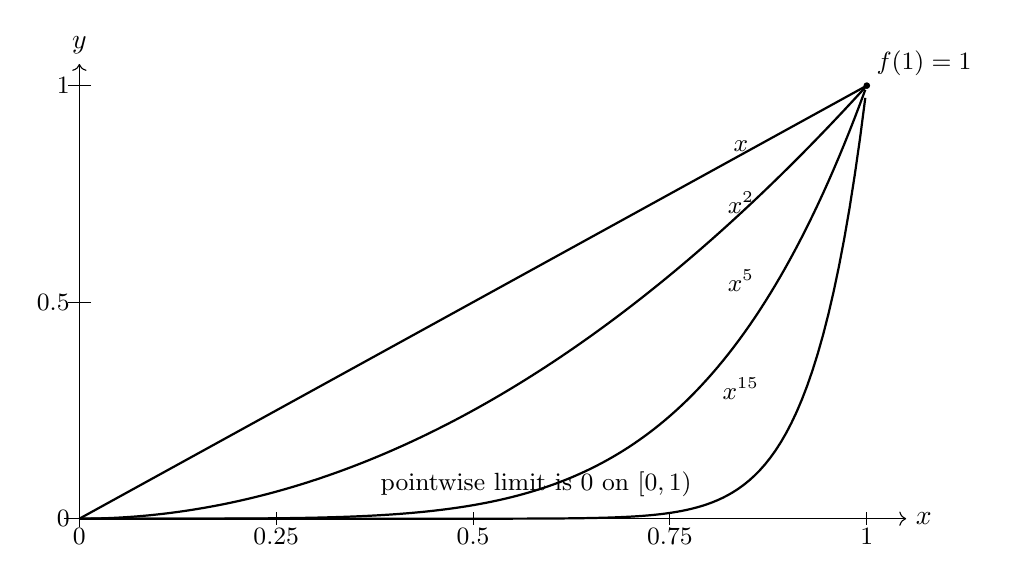
\begin{tikzpicture}[x=10cm,y=5.5cm]
  \draw[->] (-0.02,0) -- (1.05,0) node[right] {$x$};
  \draw[->] (0,-0.02) -- (0,1.05) node[above] {$y$};

  % axes ticks
  \foreach \xx/\lab in {0/0,0.25/0.25,0.5/0.5,0.75/0.75,1/1}{
    \draw (\xx,0.015) -- (\xx,-0.015);
    \node[below] at (\xx,0) {\small $\lab$};
  }
  \foreach \yy/\lab in {0/0,0.5/0.5,1/1}{
    \draw (0.015,\yy) -- (-0.015,\yy);
    \node[left] at (0,\yy) {\small $\lab$};
  }

  % plot x^n for a few n
  \draw[thick,domain=0:1,samples=150] plot (\x,{(\x)});
  \draw[thick,domain=0:1,samples=150] plot (\x,{(\x)^2});
  \draw[thick,domain=0:1,samples=150] plot (\x,{(\x)^5});
  \draw[thick,domain=0:1,samples=150] plot (\x,{(\x)^15});

  \node at (0.84,0.86) {\small $x$};
  \node at (0.84,0.73) {\small $x^2$};
  \node at (0.84,0.55) {\small $x^5$};
  \node at (0.84,0.30) {\small $x^{15}$};

  % limit function marker at (1,1)
  \fill (1,1) circle (1.2pt);
  \node[above right] at (1,1) {\small $f(1)=1$};
  \node at (0.58,0.08) {\small pointwise limit is $0$ on $[0,1)$};
\end{tikzpicture}
\caption{The functions $x^n$ collapse toward $0$ on $[0,1)$, but near $x=1$ the convergence cannot be made uniform.}
\end{figure}

\subsubsection{A Simple Uniform Convergence Example}

\begin{example}[A uniformly convergent sequence]\label{ex:uniform-simple}
Let $f_n:[0,1]\to\RR$ be
\[
f_n(x)=\frac{x}{1+n x}.
\]
Then $f_n\to 0$ uniformly on $[0,1]$.
\end{example}

\begin{proof}
For $x\in[0,1]$, we have $0\le f_n(x)\le \frac{x}{n x}=\frac{1}{n}$ for $x>0$, and also $f_n(0)=0$.
Hence
\[
\|f_n-0\|_{\infty,[0,1]}=\sup_{x\in[0,1]}\frac{x}{1+n x}=\frac{1}{1+n}\le \frac{1}{n}\to 0.
\]
So $f_n\to 0$ uniformly.
\end{proof}

\begin{exercise}
Show that if $f_n\to f$ uniformly on $D$, then $(f_n)$ is uniformly Cauchy on $D$.
Prove the converse using \Cref{thm:uniform-complete}.
\end{exercise}

\begin{exercise}
Let $f_n(x)=\frac{n x}{1+n x}$ on $[0,1]$. Find the pointwise limit and decide whether convergence is uniform.
\end{exercise}

\newpage

% -------------------------------------------------
\subsection{Uniform Convergence and Continuity}

\subsubsection{Uniform Limit of Continuous Functions}

\begin{theorem}[Uniform limit theorem for continuity]\label{thm:uniform-limit-cont}
Let $D\subseteq\RR$ and let $f_n:D\to\RR$ be continuous on $D$ for all $n$.
If $f_n\to f$ uniformly on $D$, then $f$ is continuous on $D$.
\end{theorem}

\begin{proof}
Fix $a\in D$ and $\eps>0$.
By uniform convergence, choose $N$ such that
\[
\sup_{x\in D}\abs{f_N(x)-f(x)}<\frac{\eps}{3}.
\]
Since $f_N$ is continuous at $a$, choose $\delta>0$ such that for all $x\in D$ with $\abs{x-a}<\delta$,
\[
\abs{f_N(x)-f_N(a)}<\frac{\eps}{3}.
\]
Then for $\abs{x-a}<\delta$ (with $x\in D$),
\begin{align*}
\abs{f(x)-f(a)}
&\le \abs{f(x)-f_N(x)}+\abs{f_N(x)-f_N(a)}+\abs{f_N(a)-f(a)}\\
&< \frac{\eps}{3}+\frac{\eps}{3}+\frac{\eps}{3}=\eps.
\end{align*}
This is exactly continuity of $f$ at $a$. Since $a$ was arbitrary, $f$ is continuous on $D$.
\end{proof}

\begin{remark}
Example \Cref{ex:xn} explains \emph{why} uniform convergence is needed:
each $x^n$ is continuous on $[0,1]$, but the pointwise limit is discontinuous, so the convergence cannot be uniform.
\end{remark}

\subsubsection{Uniform Convergence on Compact Sets and Uniform Continuity}

\begin{corollary}[Uniform continuity on compact domains]\label{cor:unifcont-compact}
Let $K\subseteq\RR$ be compact.
If $f_n:K\to\RR$ are continuous and $f_n\to f$ uniformly on $K$, then $f$ is uniformly continuous on $K$.
\end{corollary}

\begin{proof}
By \Cref{thm:uniform-limit-cont}, $f$ is continuous on $K$.
A continuous function on a compact set is uniformly continuous (Heine--Cantor).
\end{proof}

\subsubsection{Dini's Theorem (A Powerful Compactness Upgrade)}

\begin{theorem}[Dini's theorem]\label{thm:dini}
Let $K\subseteq\RR$ be compact.
Let $(f_n)$ be a sequence of continuous functions $f_n:K\to\RR$ such that:
\begin{enumerate}[label=(\alph*)]
\item $f_n(x)\to f(x)$ pointwise on $K$,
\item $f$ is continuous on $K$,
\item the convergence is monotone in $n$: for each $x\in K$, either
$f_1(x)\le f_2(x)\le \cdots \le f(x)$ for all $n$ (increasing case),
or $f_1(x)\ge f_2(x)\ge \cdots \ge f(x)$ for all $n$ (decreasing case).
\end{enumerate}
Then $f_n\to f$ uniformly on $K$.
\end{theorem}

\begin{proof}
We prove the increasing case; the decreasing case follows by applying the result to $-f_n$.

Fix $\eps>0$ and define
\[
E_n \coloneqq \{x\in K:\ f(x)-f_n(x)<\eps\}.
\]
Because $f-f_n$ is continuous (difference of continuous functions), $E_n$ is open in $K$ (relative topology).
Also, since $f_n(x)\uparrow f(x)$ pointwise, for every $x\in K$ there exists $n$ with $f(x)-f_n(x)<\eps$, hence
\[
K=\bigcup_{n=1}^\infty E_n.
\]
Thus $\{E_n\}_{n\in\NN}$ is an open cover of the compact set $K$, so there exists a finite subcover
$K\subseteq E_{n_1}\cup\cdots\cup E_{n_m}$.
Let $N=\max\{n_1,\dots,n_m\}$.
Since $f_n$ is increasing in $n$, we have $f_N\ge f_{n_j}$ pointwise, hence
\[
f(x)-f_N(x)\le f(x)-f_{n_j}(x)<\eps
\quad\text{whenever }x\in E_{n_j}.
\]
Because the $E_{n_j}$ cover $K$, it follows that $f(x)-f_N(x)<\eps$ for all $x\in K$, i.e.
\[
\sup_{x\in K}\abs{f(x)-f_N(x)}=\sup_{x\in K}\bigl(f(x)-f_N(x)\bigr)<\eps.
\]
Therefore $f_n\to f$ uniformly on $K$.
\end{proof}

\begin{exercise}
Let $K=[0,1]$ and $f_n(x)=x^{1/n}$. Show that $f_n\to 1$ pointwise on $(0,1]$ and $f_n(0)=0$ for all $n$.
Decide whether the convergence is uniform on $[0,1]$ and explain which hypothesis of Dini's theorem fails.
\end{exercise}

\newpage

% -------------------------------------------------
\subsection{Uniform Convergence and Integration}

\subsubsection{Interchanging Limit and Integral}

\begin{theorem}[Uniform convergence and the Riemann integral]\label{thm:unif-int}
Let $(f_n)$ be a sequence of Riemann integrable functions on $[a,b]$.
Assume $f_n\to f$ uniformly on $[a,b]$.
Then:
\begin{enumerate}[label=(\alph*)]
\item $f$ is Riemann integrable on $[a,b]$;
\item $\displaystyle \int_a^b f(x)\,\diff x = \lim_{n\to\infty}\int_a^b f_n(x)\,\diff x$.
\end{enumerate}
\end{theorem}

\begin{proof}
Let $\eps>0$.
By uniform convergence, choose $N$ such that for all $n\ge N$,
\[
\|f_n-f\|_{\infty,[a,b]}<\frac{\eps}{4(b-a)}.
\]
Fix such an $n$.
Since $f_n$ is Riemann integrable, by the Darboux criterion there exists a partition $P$ with
\[
U(f_n,P)-L(f_n,P)<\frac{\eps}{2}.
\]
For each subinterval $[x_{i-1},x_i]$ of $P$,
the sup and inf of $f$ differ from those of $f_n$ by at most $\|f-f_n\|_\infty$:
\[
M_i(f,P)\le M_i(f_n,P)+\|f-f_n\|_\infty,\qquad
m_i(f,P)\ge m_i(f_n,P)-\|f-f_n\|_\infty.
\]
Hence
\begin{align*}
U(f,P)-L(f,P)
&=\sum_{i=1}^n \bigl(M_i(f,P)-m_i(f,P)\bigr)\Delta x_i\\
&\le \sum_{i=1}^n \Bigl(\bigl(M_i(f_n,P)-m_i(f_n,P)\bigr)+2\|f-f_n\|_\infty\Bigr)\Delta x_i\\
&=\bigl(U(f_n,P)-L(f_n,P)\bigr)+2\|f-f_n\|_\infty(b-a)
<\frac{\eps}{2}+2\cdot\frac{\eps}{4(b-a)}(b-a)=\eps.
\end{align*}
So $U(f,P)-L(f,P)<\eps$, and by the Darboux criterion $f$ is integrable. This proves (a).

For (b), use the estimate
\[
\left|\int_a^b f(x)\,\diff x-\int_a^b f_n(x)\,\diff x\right|
=
\left|\int_a^b (f(x)-f_n(x))\,\diff x\right|
\le \int_a^b \abs{f(x)-f_n(x)}\,\diff x
\le (b-a)\|f-f_n\|_\infty,
\]
where the last inequality is a direct integral bound.
As $n\to\infty$, $\|f-f_n\|_\infty\to 0$, so the difference of integrals tends to $0$, proving
\[
\int_a^b f=\lim_{n\to\infty}\int_a^b f_n.
\]
\end{proof}

\subsubsection{Uniform Convergence of Series and Term-by-Term Integration}

\begin{theorem}[Term-by-term integration for uniformly convergent series]\label{thm:series-int}
Let $f_n:[a,b]\to\RR$ be Riemann integrable for all $n$.
Assume the series $\sum_{n=1}^\infty f_n$ converges uniformly on $[a,b]$ to a function $f$ (i.e.\ its partial sums converge uniformly to $f$).
Then $f$ is Riemann integrable and
\[
\int_a^b f(x)\,\diff x
=
\sum_{n=1}^\infty \int_a^b f_n(x)\,\diff x,
\]
where the series on the right converges in $\RR$.
\end{theorem}

\begin{proof}
Let $s_N=\sum_{n=1}^N f_n$.
Uniform convergence means $s_N\to f$ uniformly.
Each $s_N$ is Riemann integrable as a finite sum of integrable functions.
Apply \Cref{thm:unif-int} to $(s_N)$:
\[
\int_a^b f=\lim_{N\to\infty}\int_a^b s_N
=\lim_{N\to\infty}\sum_{n=1}^N \int_a^b f_n
=\sum_{n=1}^\infty \int_a^b f_n,
\]
where the last equality is the definition of convergence of a real series via partial sums.
\end{proof}

\begin{exercise}
Give an example of a sequence $(f_n)$ that converges pointwise on $[0,1]$ to $0$ but for which
$\int_0^1 f_n$ does not converge to $0$.
Explain precisely why this does not contradict \Cref{thm:unif-int}.
\end{exercise}

\newpage

% -------------------------------------------------
\subsection{Uniform Convergence and Differentiation}

\subsubsection{Why Differentiation is Subtle}

\begin{remark}
Unlike integration, differentiation is not continuous with respect to uniform convergence:
it is possible that $f_n\to f$ uniformly while $f_n'$ fails to converge, or converges to something different from $f'$.
To justify exchanging limit and derivative, we need \emph{additional structure}, typically uniform control of derivatives.
\end{remark}

\subsubsection{A Standard Interchange Theorem}

\begin{theorem}[Uniform convergence of derivatives]\label{thm:unif-deriv}
Let $(f_n)$ be a sequence of functions on $[a,b]$ such that:
\begin{enumerate}[label=(\alph*)]
\item each $f_n$ is differentiable on $[a,b]$ and $f_n'$ is continuous on $[a,b]$;
\item $(f_n')$ converges uniformly on $[a,b]$ to a function $g$;
\item there exists $x_0\in[a,b]$ such that $(f_n(x_0))$ converges in $\RR$.
\end{enumerate}
Then:
\begin{enumerate}[label=(\roman*)]
\item there exists a function $f:[a,b]\to\RR$ such that $f_n\to f$ uniformly on $[a,b]$;
\item $f$ is differentiable on $[a,b]$ (on $(a,b)$ in the classical sense) and $f'(x)=g(x)$ for all $x\in[a,b]$;
\item in particular, $g$ is continuous (as a uniform limit of continuous functions).
\end{enumerate}
\end{theorem}

\begin{proof}
Fix $x\in[a,b]$. By the Fundamental Theorem of Calculus applied to $f_n'$ (continuous),
\[
f_n(x)-f_n(x_0)=\int_{x_0}^{x} f_n'(t)\,\diff t.
\]
Let $n,m\in\NN$. Subtract the corresponding identities:
\[
f_n(x)-f_m(x)
=
\bigl(f_n(x_0)-f_m(x_0)\bigr)+\int_{x_0}^{x}\bigl(f_n'(t)-f_m'(t)\bigr)\,\diff t.
\]
Take absolute values and use the integral bound:
\begin{align*}
\abs{f_n(x)-f_m(x)}
&\le \abs{f_n(x_0)-f_m(x_0)}
+\int_{x_0}^{x}\abs{f_n'(t)-f_m'(t)}\,\diff t\\
&\le \abs{f_n(x_0)-f_m(x_0)} + (b-a)\,\|f_n'-f_m'\|_{\infty,[a,b]}.
\end{align*}
Now take the supremum over $x\in[a,b]$:
\[
\|f_n-f_m\|_{\infty,[a,b]}
\le \abs{f_n(x_0)-f_m(x_0)} + (b-a)\,\|f_n'-f_m'\|_{\infty,[a,b]}.
\]
By hypothesis, $(f_n(x_0))$ converges, hence is Cauchy, so the first term can be made small for large $m,n$.
Also, uniform convergence of $f_n'$ implies $(f_n')$ is uniformly Cauchy, so the second term can be made small.
Therefore $(f_n)$ is uniformly Cauchy, and by \Cref{thm:uniform-complete} there exists $f$ such that $f_n\to f$ uniformly.
This proves (i).

Next, we show $f'=g$.
Fix $x\in[a,b]$ and write, again using FTC,
\[
f_n(x)-f_n(x_0)=\int_{x_0}^{x} f_n'(t)\,\diff t.
\]
Let $n\to\infty$.
Uniform convergence $f_n\to f$ implies the left-hand side tends to $f(x)-f(x_0)$.
Uniform convergence $f_n'\to g$ and \Cref{thm:unif-int} imply
\[
\int_{x_0}^{x} f_n'(t)\,\diff t \to \int_{x_0}^{x} g(t)\,\diff t.
\]
Hence for all $x\in[a,b]$,
\[
f(x)-f(x_0)=\int_{x_0}^{x} g(t)\,\diff t.
\]
Define $G(x)=\int_{x_0}^{x} g(t)\,\diff t$.
Since $g$ is continuous (uniform limit of continuous functions), FTC I yields $G'(x)=g(x)$ for $x\in(a,b)$.
Because $f(x)=f(x_0)+G(x)$, we obtain $f'(x)=g(x)$ on $(a,b)$.
This proves (ii), and (iii) has already been noted.
\end{proof}

\subsubsection{A Cautionary Example}

\begin{example}[Uniform convergence does not justify termwise differentiation]
Define $f_n:[0,1]\to\RR$ by
\[
f_n(x)=\sqrt{x^2+\frac{1}{n}}.
\]
Then $f_n\to f$ uniformly on $[0,1]$ where $f(x)=x$.
Indeed,
\[
0\le f_n(x)-x=\sqrt{x^2+\frac{1}{n}}-x
=\frac{\frac{1}{n}}{\sqrt{x^2+\frac{1}{n}}+x}
\le \frac{\frac{1}{n}}{\sqrt{\frac{1}{n}}}=\frac{1}{\sqrt{n}},
\]
so $\|f_n-f\|_\infty\le 1/\sqrt{n}\to 0$.

However,
\[
f_n'(x)=\frac{x}{\sqrt{x^2+\frac{1}{n}}},
\]
and while $f_n'(x)\to 1$ for every $x>0$, we have $f_n'(0)=0$ for all $n$.
Thus $f_n'$ does not converge pointwise to $f'(x)=1$ on all of $[0,1]$, and certainly not uniformly.
This illustrates why \Cref{thm:unif-deriv} needs uniform convergence of derivatives (or comparable hypotheses).
\end{example}

\begin{exercise}
Let $f_n(x)=\frac{\sin(nx)}{n}$ on $[0,2\pi]$.
Show that $f_n\to 0$ uniformly, but $f_n'(x)=\cos(nx)$ does not converge pointwise.
\end{exercise}

\newpage

% -------------------------------------------------
\subsection{Series of Functions and the Weierstrass \texorpdfstring{$M$}{M}-Test}

\subsubsection{Uniform Convergence of Series}

\begin{definition}[Series of functions]\label{def:series-fn}
Let $f_n:D\to\RR$. Define partial sums
\[
s_N(x)\coloneqq \sum_{n=1}^{N} f_n(x).
\]
We say $\sum_{n=1}^\infty f_n$ \emph{converges pointwise} on $D$ if $s_N(x)$ converges for each fixed $x$.
It \emph{converges uniformly} on $D$ if $s_N\to s$ uniformly on $D$ for some function $s$.
\end{definition}

\subsubsection{Weierstrass M-Test}

\begin{theorem}[Weierstrass $M$-test]\label{thm:mtest}
Let $f_n:D\to\RR$ and suppose there exist numbers $M_n\ge 0$ such that for all $x\in D$,
\[
\abs{f_n(x)}\le M_n.
\]
If the numerical series $\sum_{n=1}^\infty M_n$ converges, then $\sum_{n=1}^\infty f_n$ converges uniformly (and absolutely) on $D$.
\end{theorem}

\begin{proof}
Let $s_N=\sum_{n=1}^N f_n$.
For $m>n$ and any $x\in D$,
\[
\abs{s_m(x)-s_n(x)}
=\abs{\sum_{k=n+1}^{m} f_k(x)}
\le \sum_{k=n+1}^{m}\abs{f_k(x)}
\le \sum_{k=n+1}^{m} M_k.
\]
Taking the supremum over $x\in D$ yields
\[
\|s_m-s_n\|_{\infty,D}\le \sum_{k=n+1}^{m} M_k.
\]
Since $\sum M_k$ converges, its tails go to $0$, hence $(s_N)$ is uniformly Cauchy.
By \Cref{thm:uniform-complete}, $s_N$ converges uniformly on $D$.
\end{proof}

\subsubsection{Consequences: Continuity and Integration Term-by-Term}

\begin{corollary}[Uniformly convergent series of continuous functions]\label{cor:series-cont}
If each $f_n$ is continuous on $D$ and $\sum f_n$ converges uniformly on $D$, then the sum function $s$ is continuous on $D$.
\end{corollary}

\begin{proof}
The partial sums $s_N$ are continuous as finite sums of continuous functions.
Uniform convergence $s_N\to s$ and \Cref{thm:uniform-limit-cont} imply $s$ is continuous.
\end{proof}

\begin{corollary}[Term-by-term integration on {$[a,b]$}]\label{cor:series-int2}
If each $f_n$ is Riemann integrable on $[a,b]$ and $\sum f_n$ converges uniformly...
\[
\int_a^b s(x)\,\diff x=\sum_{n=1}^\infty \int_a^b f_n(x)\,\diff x.
\]
\end{corollary}

\begin{proof}
This is exactly \Cref{thm:series-int}.
\end{proof}

\begin{exercise}
Use the $M$-test to show that $\sum_{n=1}^\infty \frac{\sin(nx)}{n^2}$ converges uniformly on $\RR$.
Deduce that its sum is continuous on $\RR$.
\end{exercise}

\newpage

% -------------------------------------------------
\subsection{Power Series as a Primary Source of Uniform Convergence}

\subsubsection{Uniform Convergence on Compact Subintervals}

\begin{theorem}[Uniform convergence inside the radius]\label{thm:power-uniform}
Let $\sum_{n=0}^\infty c_n(x-x_0)^n$ be a power series with radius of convergence $R>0$.
Fix $r$ with $0<r<R$ and set $K=[x_0-r,x_0+r]$.
Then the power series converges uniformly on $K$.
\end{theorem}

\begin{proof}
Because $r<R$, the series $\sum_{n=0}^\infty \abs{c_n}r^n$ converges (absolute convergence at any point with $\abs{x-x_0}=r$ is not guaranteed,
but convergence of $\sum \abs{c_n}r^n$ follows from the definition of radius; equivalently, apply the root test with $\abs{x-x_0}=r<R$).

For $x\in K$ we have $\abs{x-x_0}\le r$, hence
\[
\abs{c_n(x-x_0)^n}\le \abs{c_n}r^n.
\]
By the Weierstrass $M$-test (\Cref{thm:mtest}) with $M_n=\abs{c_n}r^n$, the power series converges uniformly on $K$.
\end{proof}

\subsubsection{Term-by-Term Differentiation and Integration of Power Series}

\begin{theorem}[Differentiating and integrating power series]\label{thm:power-termwise}
Let $\sum_{n=0}^\infty c_n(x-x_0)^n$ have radius of convergence $R>0$.
Define
\[
S(x)\coloneqq \sum_{n=0}^\infty c_n(x-x_0)^n \qquad (\abs{x-x_0}<R).
\]
Then:
\begin{enumerate}[label=(\alph*)]
\item $S$ is differentiable on $(x_0-R,x_0+R)$ and
\[
S'(x)=\sum_{n=1}^\infty n c_n (x-x_0)^{n-1},\qquad \abs{x-x_0}<R.
\]
\item $S$ is Riemann integrable on every $[x_0-r,x_0+r]$ with $0<r<R$ and
\[
\int_{x_0}^{x} S(t)\,\diff t
=
\sum_{n=0}^\infty c_n \int_{x_0}^{x} (t-x_0)^n\,\diff t
=
\sum_{n=0}^\infty c_n \frac{(x-x_0)^{n+1}}{n+1},
\qquad \abs{x-x_0}<R.
\]
\end{enumerate}
Moreover, the differentiated and integrated series have the same radius of convergence $R$.
\end{theorem}

\begin{proof}
Fix $r$ with $0<r<R$ and work on $K=[x_0-r,x_0+r]$.

\textbf{(a) Differentiation.}
Consider the partial sums
\[
S_N(x)=\sum_{n=0}^{N} c_n(x-x_0)^n,
\qquad
S_N'(x)=\sum_{n=1}^{N} n c_n(x-x_0)^{n-1}.
\]
Each $S_N$ is $C^1$ and $S_N'$ is continuous.
We will show $S_N'\to G$ uniformly on $K$ for
\[
G(x)\coloneqq \sum_{n=1}^\infty n c_n(x-x_0)^{n-1}.
\]
For $x\in K$,
\[
\abs{n c_n(x-x_0)^{n-1}}\le n\abs{c_n}\,r^{n-1}.
\]
The numerical series $\sum_{n=1}^\infty n\abs{c_n}\,r^{n-1}$ converges because the original power series converges absolutely for any $\rho$ with $r<\rho<R$
and one can compare using standard ratio/root test arguments; concretely, since $\sum \abs{c_n}\rho^n$ converges,
we have $\abs{c_n}\rho^n\to 0$, and the ratio test implies $\sum n\abs{c_n}r^{n-1}$ converges for $r<\rho<R$.
Thus by the $M$-test, $S_N'\to G$ uniformly on $K$.

Also, $S_N(x_0)=c_0$ for all $N$, so $(S_N(x_0))$ converges.
Therefore, by \Cref{thm:unif-deriv}, $S_N\to S$ uniformly on $K$ and $S$ is differentiable on $K$ with $S'=G$ on the interior.
Since $r<R$ was arbitrary, this holds for all $\abs{x-x_0}<R$.

\textbf{(b) Integration.}
By \Cref{thm:power-uniform}, $S_N\to S$ uniformly on $K$, and each $S_N$ is continuous hence Riemann integrable.
By \Cref{thm:unif-int},
\[
\int_{x_0}^{x} S(t)\,\diff t
=
\lim_{N\to\infty}\int_{x_0}^{x} S_N(t)\,\diff t
=
\lim_{N\to\infty}\sum_{n=0}^{N} c_n \int_{x_0}^{x}(t-x_0)^n\,\diff t,
\]
and the integral of $(t-x_0)^n$ is $\frac{(x-x_0)^{n+1}}{n+1}$.
Thus the integrated series representation follows.

The statement about radius of convergence is standard: differentiating or integrating a power series does not change the radius,
because multiplying coefficients by $n$ or dividing by $n+1$ does not affect the $\limsup$ in the root test.
\end{proof}

\begin{exercise}
Let $S(x)=\sum_{n=0}^\infty x^n$ for $\abs{x}<1$.
Use \Cref{thm:power-termwise} to justify differentiating term-by-term and show
\[
\sum_{n=1}^\infty n x^{n-1}=\frac{1}{(1-x)^2},\qquad \abs{x}<1.
\]
Then integrate to obtain $\sum_{n=1}^\infty \frac{x^n}{n}=-\log(1-x)$ for $\abs{x}<1$.
\end{exercise}

\begin{exercise}
Let $f_n(x)=\frac{x^n}{n}$ on $[0,1]$. Show that $\sum_{n=1}^\infty f_n(x)$ converges for each $x\in[0,1)$ but not uniformly on $[0,1)$.
Decide whether it converges uniformly on $[0,r]$ for each $r<1$.
\end{exercise}

\newpage

% =========================
% Metric Spaces (Revised: unique labels)
% =========================

\section{Metric Spaces}

\begin{keyidea}
A metric space is the minimal framework needed to discuss \emph{distance}, \emph{limits},
\emph{continuity}, \emph{Cauchy sequences}, \emph{completeness}, and \emph{compactness}.
Many theorems from $\RR$ extend verbatim once we identify which properties of $\RR$ the proof actually uses
(e.g.\ the triangle inequality, completeness, compactness).
\end{keyidea}

% -------------------------------------------------
\subsection{Metrics and Basic Geometry}

\subsubsection{Definition and Examples}

\begin{definition}[Metric space]\label{ms:def:metric-space}
A \emph{metric space} is a pair $(X,d)$ where $X$ is a nonempty set and
$d:X\times X\to[0,\infty)$ satisfies, for all $x,y,z\in X$:
\begin{enumerate}[label=(\alph*)]
\item \textbf{Positivity:} $d(x,y)\ge 0$, and $d(x,y)=0$ if and only if $x=y$.
\item \textbf{Symmetry:} $d(x,y)=d(y,x)$.
\item \textbf{Triangle inequality:} $d(x,z)\le d(x,y)+d(y,z)$.
\end{enumerate}
\end{definition}

\begin{proposition}[Reverse triangle inequality]\label{ms:prop:reverse-triangle}
For all $x,y,z\in X$,
\[
\abs{d(x,z)-d(y,z)}\le d(x,y).
\]
\end{proposition}

\begin{proof}
By the triangle inequality,
\[
d(x,z)\le d(x,y)+d(y,z)\quad\Rightarrow\quad d(x,z)-d(y,z)\le d(x,y).
\]
Swap $x$ and $y$ to get $d(y,z)-d(x,z)\le d(x,y)$.
Combine both inequalities.
\end{proof}

\begin{example}[$\RR$ with the usual metric]\label{ms:ex:R}
On $\RR$, $d(x,y)=\abs{x-y}$ is a metric.
\end{example}

\begin{example}[$\RR^n$ with common metrics]\label{ms:ex:Rn-metrics}
For $x,y\in\RR^n$ define
\[
d_2(x,y)=\left(\sum_{k=1}^n (x_k-y_k)^2\right)^{1/2},\qquad
d_1(x,y)=\sum_{k=1}^n \abs{x_k-y_k},\qquad
d_\infty(x,y)=\max_{1\le k\le n}\abs{x_k-y_k}.
\]
Each is a metric on $\RR^n$.
\end{example}

\begin{example}[Discrete metric]\label{ms:ex:discrete}
On any set $X$, the function
\[
d(x,y)=
\casesm{
0, & x=y,\\
1, & x\neq y,
}
\]
is a metric. This space is called \emph{discrete}.
\end{example}

\begin{example}[Subspace metric]\label{ms:ex:subspace}
If $(X,d)$ is a metric space and $Y\subseteq X$, then
\[
d_Y(y_1,y_2)\coloneqq d(y_1,y_2)\qquad (y_1,y_2\in Y)
\]
is a metric on $Y$. We call it the \emph{subspace metric}.
\end{example}

\subsubsection{Equivalent Metrics}

\begin{definition}[Equivalent metrics]\label{ms:def:equiv-metric}
Two metrics $d$ and $\rho$ on the same set $X$ are \emph{(topologically) equivalent} if they generate the same open sets
(equivalently, the same convergent sequences).
\end{definition}

\begin{proposition}[Bi-Lipschitz comparison implies equivalence]\label{ms:prop:bilip-equivalence}
If there exist constants $c,C>0$ such that for all $x,y\in X$,
\[
c\,d(x,y)\le \rho(x,y)\le C\,d(x,y),
\]
then $d$ and $\rho$ are equivalent.
\end{proposition}

\begin{proof}
Fix $x\in X$ and $r>0$.
If $\rho(x,y)<r$, then $c\,d(x,y)\le \rho(x,y)<r$, hence $d(x,y)<r/c$, so
\[
B_\rho(x,r)\subseteq B_d\!\left(x,\frac{r}{c}\right).
\]
Similarly, if $d(x,y)<r$, then $\rho(x,y)\le C\,d(x,y)<Cr$, so
\[
B_d(x,r)\subseteq B_\rho(x,Cr).
\]
Thus each $\rho$-ball contains a $d$-ball around the same center and vice versa, which implies the induced open sets coincide.
\end{proof}

\begin{remark}
On $\RR^n$, the metrics $d_1,d_2,d_\infty$ are equivalent.
For instance, for all $v\in\RR^n$,
\[
\|v\|_\infty \le \|v\|_2 \le \sqrt{n}\,\|v\|_\infty,
\qquad
\|v\|_2 \le \|v\|_1 \le \sqrt{n}\,\|v\|_2,
\]
which yields inequalities of the form in \Cref{ms:prop:bilip-equivalence}.
\end{remark}

% -------------------------------------------------
\subsection{Open Balls, Open Sets, and Closed Sets}

\subsubsection{Balls and the Induced Topology}

\begin{definition}[Open and closed balls]\label{ms:def:ball}
Let $(X,d)$ be a metric space, $x\in X$, and $r>0$.
\[
B(x,r)\coloneqq \{y\in X:\ d(x,y)<r\},\qquad
\overline{B}(x,r)\coloneqq \{y\in X:\ d(x,y)\le r\}.
\]
\end{definition}

\begin{proposition}[Open balls are open]\label{ms:prop:balls-open}
For every $x\in X$ and $r>0$, the set $B(x,r)$ is open.
\end{proposition}

\begin{proof}
Let $y\in B(x,r)$, so $d(x,y)<r$. Define $\eps\coloneqq r-d(x,y)>0$.
If $z\in B(y,\eps)$ then by the triangle inequality,
\[
d(x,z)\le d(x,y)+d(y,z)<d(x,y)+\eps=r,
\]
so $z\in B(x,r)$. Hence $B(y,\eps)\subseteq B(x,r)$, proving $B(x,r)$ is open.
\end{proof}

\begin{definition}[Open set]\label{ms:def:open-set}
A set $U\subseteq X$ is \emph{open} if for every $x\in U$ there exists $r>0$ such that $B(x,r)\subseteq U$.
\end{definition}

\begin{proposition}[Open set axioms]\label{ms:prop:open-axioms}
\begin{enumerate}[label=(\alph*)]
\item $\emptyset$ and $X$ are open.
\item Arbitrary unions of open sets are open.
\item Finite intersections of open sets are open.
\end{enumerate}
\end{proposition}

\begin{proof}
(a) is immediate.
(b) If $x\in\bigcup_\alpha U_\alpha$, then $x\in U_{\alpha_0}$ for some $\alpha_0$; take a ball inside $U_{\alpha_0}$.
(c) If $x\in U\cap V$ with $U,V$ open, choose radii $r_U,r_V$ with $B(x,r_U)\subseteq U$ and $B(x,r_V)\subseteq V$.
Then $B(x,\min\{r_U,r_V\})\subseteq U\cap V$.
\end{proof}

\subsubsection{Closed Sets and a Sequential Characterization}

\begin{definition}[Closed set]\label{ms:def:closed-set}
A set $F\subseteq X$ is \emph{closed} if $X\setminus F$ is open.
\end{definition}

\begin{proposition}[Closed $\Leftrightarrow$ sequentially closed]\label{ms:prop:closed-seq}
A set $F\subseteq X$ is closed if and only if it contains the limits of all convergent sequences from $F$:
whenever $x_n\in F$ and $x_n\to x$ in $X$, we have $x\in F$.
\end{proposition}

\begin{proof}
($\Rightarrow$) Suppose $F$ is closed and $x_n\in F$ with $x_n\to x$.
If $x\notin F$, then $x\in X\setminus F$, which is open, so there exists $r>0$ with $B(x,r)\subseteq X\setminus F$.
But $x_n\to x$ implies $x_n\in B(x,r)$ for all large $n$, contradicting $x_n\in F$. Hence $x\in F$.

($\Leftarrow$) Suppose the sequential property holds and $X\setminus F$ is not open.
Then there exists $x\in X\setminus F$ such that for every $n$ there exists $x_n\in F$ with $d(x_n,x)<1/n$.
Thus $x_n\to x$ with $x_n\in F$, forcing $x\in F$, a contradiction. Hence $X\setminus F$ is open and $F$ is closed.
\end{proof}

\begin{figure}[H]
\centering
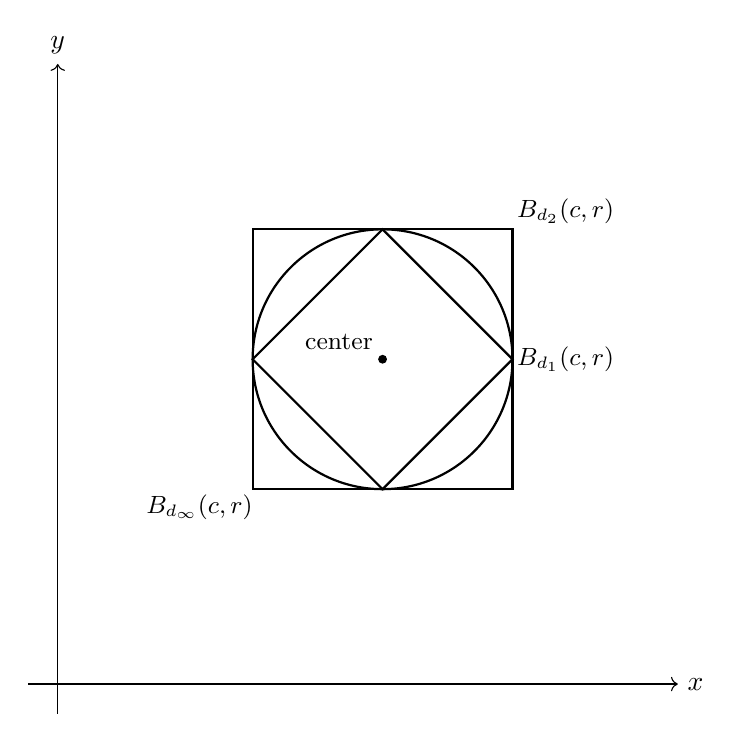
\begin{tikzpicture}[x=7.5cm,y=7.5cm]
  \draw[->] (-0.05,0) -- (1.05,0) node[right] {$x$};
  \draw[->] (0,-0.05) -- (0,1.05) node[above] {$y$};

  \coordinate (c) at (0.55,0.55);
  \fill (c) circle (1.6pt);
  \node[above left] at (c) {\small center};

  % Euclidean ball (circle)
  \draw[thick] (c) circle (0.22);
  \node at (0.86,0.80) {\small $B_{d_2}(c,r)$};

  % l1 ball (diamond)
  \draw[thick] (0.55,0.77) -- (0.77,0.55) -- (0.55,0.33) -- (0.33,0.55) -- cycle;
  \node at (0.86,0.55) {\small $B_{d_1}(c,r)$};

  % linfty ball (square)
  \draw[thick] (0.33,0.33) rectangle (0.77,0.77);
  \node at (0.24,0.30) {\small $B_{d_\infty}(c,r)$};
\end{tikzpicture}
\caption{In $\RR^2$, the shape of a ball depends on the metric: circle ($d_2$), diamond ($d_1$), square ($d_\infty$). These metrics are equivalent, so they generate the same open sets.}
\end{figure}

% -------------------------------------------------
\subsection{Convergence, Continuity, and Completeness}

\subsubsection{Convergent and Cauchy Sequences}

\begin{definition}[Convergence]\label{ms:def:convergence}
A sequence $(x_n)$ in $(X,d)$ converges to $x\in X$ (written $x_n\to x$) if
\[
\forall \eps>0\ \exists N\ \forall n\ge N,\quad d(x_n,x)<\eps.
\]
\end{definition}

\begin{proposition}[Limits are unique]\label{ms:prop:unique-limit}
If $x_n\to x$ and $x_n\to y$, then $x=y$.
\end{proposition}

\begin{proof}
Fix $\eps>0$. Choose $N_1$ with $d(x_n,x)<\eps/2$ for $n\ge N_1$ and $N_2$ with $d(x_n,y)<\eps/2$ for $n\ge N_2$.
Then for $n\ge \max\{N_1,N_2\}$,
\[
d(x,y)\le d(x,x_n)+d(x_n,y)<\frac{\eps}{2}+\frac{\eps}{2}=\eps.
\]
Since $\eps$ is arbitrary, $d(x,y)=0$ and $x=y$.
\end{proof}

\begin{definition}[Cauchy sequence]\label{ms:def:cauchy}
A sequence $(x_n)$ is \emph{Cauchy} if
\[
\forall \eps>0\ \exists N\ \forall m,n\ge N,\quad d(x_n,x_m)<\eps.
\]
\end{definition}

\begin{proposition}[Convergent $\Rightarrow$ Cauchy]\label{ms:prop:conv-implies-cauchy}
Every convergent sequence in a metric space is Cauchy.
\end{proposition}

\begin{proof}
If $x_n\to x$, choose $N$ with $d(x_n,x)<\eps/2$ for $n\ge N$. Then for $m,n\ge N$,
\[
d(x_n,x_m)\le d(x_n,x)+d(x,x_m)<\frac{\eps}{2}+\frac{\eps}{2}=\eps.
\]
\end{proof}

\subsubsection{Continuity}

\begin{definition}[Continuity between metric spaces]\label{ms:def:continuity}
Let $(X,d_X)$ and $(Y,d_Y)$ be metric spaces and $f:X\to Y$.
We say $f$ is \emph{continuous at} $x\in X$ if
\[
\forall \eps>0\ \exists \delta>0\ \forall x'\in X,\quad
d_X(x',x)<\delta \Rightarrow d_Y\bigl(f(x'),f(x)\bigr)<\eps.
\]
\end{definition}

\begin{theorem}[Sequential characterization of continuity]\label{ms:thm:cont-seq}
$f$ is continuous at $x$ if and only if for every sequence $x_n\to x$ in $X$, we have $f(x_n)\to f(x)$ in $Y$.
\end{theorem}

\begin{proof}
($\Rightarrow$) Let $x_n\to x$ and fix $\eps>0$. Choose $\delta$ from continuity at $x$.
Then for large $n$, $d_X(x_n,x)<\delta$, hence $d_Y(f(x_n),f(x))<\eps$.

($\Leftarrow$) If $f$ is not continuous at $x$, there exists $\eps_0>0$ such that for every $k\in\NN$ there is $x_k$ with
$d_X(x_k,x)<1/k$ but $d_Y(f(x_k),f(x))\ge \eps_0$.
Then $x_k\to x$ but $f(x_k)\not\to f(x)$, contradicting the sequential property.
\end{proof}

\begin{theorem}[Open-set characterization]\label{ms:thm:cont-open-preimage}
A function $f:X\to Y$ is continuous on $X$ if and only if for every open set $U\subseteq Y$, the preimage $f^{-1}(U)$ is open in $X$.
\end{theorem}

\begin{proof}
($\Rightarrow$) Let $U$ be open in $Y$ and $x\in f^{-1}(U)$. Then $f(x)\in U$, so there exists $\eps>0$ with
$B_Y(f(x),\eps)\subseteq U$. Continuity gives $\delta>0$ such that
$d_X(x',x)<\delta\Rightarrow d_Y(f(x'),f(x))<\eps$, hence $f(x')\in U$.
Thus $B_X(x,\delta)\subseteq f^{-1}(U)$, so $f^{-1}(U)$ is open.

($\Leftarrow$) Fix $x\in X$ and $\eps>0$. The ball $B_Y(f(x),\eps)$ is open, so $f^{-1}(B_Y(f(x),\eps))$ is open and contains $x$.
Thus it contains some $B_X(x,\delta)$, which is exactly continuity at $x$.
\end{proof}

\subsubsection{Completeness}

\begin{definition}[Complete metric space]\label{ms:def:complete}
A metric space $(X,d)$ is \emph{complete} if every Cauchy sequence in $X$ converges to a limit in $X$.
\end{definition}

\begin{example}[$\RR$ is complete; $\QQ$ is not]\label{ms:ex:R-complete-Q-not}
$(\RR,\abs{\cdot})$ is complete.
$(\QQ,\abs{\cdot})$ is not complete: there are Cauchy sequences of rationals converging in $\RR$ to irrational limits (e.g.\ to $\sqrt2$).
\end{example}

\begin{proposition}[Closed subspaces of complete spaces are complete]\label{ms:prop:closed-complete}
Let $(X,d)$ be complete and let $F\subseteq X$ with the subspace metric.
Then $F$ is complete if and only if $F$ is closed in $X$.
\end{proposition}

\begin{proof}
($\Leftarrow$) If $F$ is closed and $(x_n)$ is Cauchy in $F$, then it is Cauchy in $X$ and hence converges to some $x\in X$.
Since $F$ is closed and $x_n\in F$, \Cref{ms:prop:closed-seq} implies $x\in F$. Thus $F$ is complete.

($\Rightarrow$) If $F$ is complete and $x_n\in F$ with $x_n\to x$ in $X$, then $(x_n)$ is Cauchy in $F$.
Completeness gives a limit $y\in F$ with $x_n\to y$ in $F$, hence also in $X$.
By uniqueness of limits (\Cref{ms:prop:unique-limit}), $x=y\in F$, so $F$ is closed.
\end{proof}

% -------------------------------------------------
\subsection{Compactness in Metric Spaces}

\subsubsection{Definitions}

\begin{definition}[Compactness (open covers)]\label{ms:def:compact}
A subset $K\subseteq X$ is \emph{compact} if every open cover of $K$ has a finite subcover:
if $\{U_\alpha\}_{\alpha\in A}$ are open in $X$ and
\[
K\subseteq \bigcup_{\alpha\in A} U_\alpha,
\]
then there exist $\alpha_1,\dots,\alpha_m$ such that
\[
K\subseteq U_{\alpha_1}\cup\cdots\cup U_{\alpha_m}.
\]
\end{definition}

\begin{definition}[Sequential compactness]\label{ms:def:seq-compact}
A set $K\subseteq X$ is \emph{sequentially compact} if every sequence in $K$ has a convergent subsequence
whose limit lies in $K$.
\end{definition}

\subsubsection{Compactness and Sequential Compactness}

\begin{lemma}[Infinite sets in compact metric spaces have accumulation points]\label{ms:lem:accumulation}
If $K$ is compact and $A\subseteq K$ is infinite, then $A$ has an accumulation point in $K$:
there exists $x\in K$ such that every ball $B(x,r)$ contains infinitely many points of $A$.
\end{lemma}

\begin{proof}
Assume for contradiction that $A$ has no accumulation point in $K$.
Then for each $x\in K$ there exists $r_x>0$ such that $B(x,r_x)$ contains only finitely many points of $A$.
The family $\{B(x,r_x)\}_{x\in K}$ is an open cover of $K$, hence has a finite subcover
$K\subseteq \bigcup_{j=1}^m B(x_j,r_{x_j})$.
But then
\[
A \subseteq \bigcup_{j=1}^m \bigl(A\cap B(x_j,r_{x_j})\bigr),
\]
a finite union of finite sets, hence finite, contradicting that $A$ is infinite.
\end{proof}

\begin{theorem}[Compact $\Longleftrightarrow$ sequentially compact (metric spaces)]\label{ms:thm:compact-seqcompact}
Let $(X,d)$ be a metric space and $K\subseteq X$. Then
\[
K \text{ is compact } \quad\Longleftrightarrow\quad K \text{ is sequentially compact.}
\]
\end{theorem}

\begin{proof}
($\Rightarrow$) Assume $K$ is compact and let $(x_n)$ be a sequence in $K$.
If $\{x_n:n\in\NN\}$ is finite, some value repeats infinitely often, giving a constant subsequence.
If it is infinite, apply \Cref{ms:lem:accumulation} to the infinite set $A=\{x_n:n\in\NN\}$ to obtain an accumulation point $x\in K$.
For each $k\in\NN$, the ball $B(x,1/k)$ contains infinitely many points of $A$,
so we can choose indices $n_1<n_2<\cdots$ such that $x_{n_k}\in B(x,1/k)$.
Then $d(x_{n_k},x)<1/k\to 0$, so $x_{n_k}\to x$ with $x\in K$. Hence $K$ is sequentially compact.

($\Leftarrow$) Assume $K$ is sequentially compact and let $\{U_\alpha\}_{\alpha\in A}$ be an open cover of $K$.
Suppose no finite subcover exists. We inductively construct a sequence $(x_n)$ in $K$ as follows:
choose $x_1\in K$ and pick $U_{\alpha_1}$ with $x_1\in U_{\alpha_1}$.
Since $\{U_\alpha\}$ has no finite subcover, $K\setminus U_{\alpha_1}\neq\emptyset$, so choose $x_2\in K\setminus U_{\alpha_1}$
and pick $U_{\alpha_2}$ with $x_2\in U_{\alpha_2}$.
Continue: having chosen $x_n$ and $U_{\alpha_n}$, since $U_{\alpha_1}\cup\cdots\cup U_{\alpha_n}$ does not cover $K$,
choose
\[
x_{n+1}\in K\setminus\bigl(U_{\alpha_1}\cup\cdots\cup U_{\alpha_n}\bigr),
\]
and then select $U_{\alpha_{n+1}}$ containing $x_{n+1}$.

By construction, for each fixed $j$, all terms $x_n$ with $n>j$ lie outside $U_{\alpha_j}$.
If $(x_{n_k})$ were a convergent subsequence with limit $x\in K$, then $x\in U_{\alpha_j}$ for some $j$
because the sets cover $K$.
Since $U_{\alpha_j}$ is open, eventually $x_{n_k}\in U_{\alpha_j}$, contradicting that all $x_n$ for $n>j$ lie outside $U_{\alpha_j}$.
Thus the sequence has no convergent subsequence, contradicting sequential compactness.
Therefore a finite subcover must exist and $K$ is compact.
\end{proof}

\subsubsection{Total Boundedness and a Useful Characterization}

\begin{definition}[Totally bounded]\label{ms:def:totally-bounded}
A subset $K\subseteq X$ is \emph{totally bounded} if for every $\eps>0$ there exist finitely many points $x_1,\dots,x_N\in X$ such that
\[
K\subseteq \bigcup_{j=1}^N B(x_j,\eps).
\]
\end{definition}

\begin{proposition}[Compact $\Rightarrow$ totally bounded]\label{ms:prop:compact-totally-bounded}
If $K$ is compact, then $K$ is totally bounded.
\end{proposition}

\begin{proof}
Fix $\eps>0$. The family $\{B(x,\eps)\}_{x\in K}$ is an open cover of $K$.
Compactness gives a finite subcover, which is exactly total boundedness.
\end{proof}

\begin{proposition}[Compact $\Rightarrow$ complete]\label{ms:prop:compact-complete}
If $K$ is compact (with the subspace metric), then $K$ is complete.
\end{proposition}

\begin{proof}
By \Cref{ms:thm:compact-seqcompact}, $K$ is sequentially compact.
Let $(x_n)$ be Cauchy in $K$. Sequential compactness gives a convergent subsequence $x_{n_k}\to x\in K$.
Fix $\eps>0$ and choose $N$ such that $d(x_n,x_m)<\eps/2$ for all $n,m\ge N$.
Choose $k$ with $n_k\ge N$ and $d(x_{n_k},x)<\eps/2$. Then for $n\ge N$,
\[
d(x_n,x)\le d(x_n,x_{n_k})+d(x_{n_k},x)<\frac{\eps}{2}+\frac{\eps}{2}=\eps,
\]
so $x_n\to x$. Thus every Cauchy sequence converges in $K$.
\end{proof}

\begin{theorem}[Complete + totally bounded $\Longleftrightarrow$ compact]\label{ms:thm:complete-totally-bounded}
A subset $K\subseteq X$ is compact if and only if it is complete and totally bounded (with the subspace metric).
\end{theorem}

\begin{proof}
($\Rightarrow$) If $K$ is compact, it is totally bounded by \Cref{ms:prop:compact-totally-bounded}
and complete by \Cref{ms:prop:compact-complete}.

($\Leftarrow$) Assume $K$ is complete and totally bounded.
Let $(x_n)$ be any sequence in $K$.
We will build a Cauchy subsequence.

By total boundedness with $\eps=1$, cover $K$ by finitely many balls of radius $1$.
One such ball contains infinitely many terms of $(x_n)$; pass to a subsequence inside it.
Next cover $K$ by finitely many balls of radius $1/2$ and pass to a further subsequence contained in one such ball.
Continue inductively to obtain nested subsequences; choose a diagonal subsequence $(y_k)$ such that
for each $m$, all sufficiently large $k$ satisfy $y_k\in B(z_m,2^{-m})$ for some center $z_m$.

Then for $k,\ell$ sufficiently large (depending on $m$), both $y_k$ and $y_\ell$ lie in the same ball of radius $2^{-m}$, hence
\[
d(y_k,y_\ell)\le 2\cdot 2^{-m}=2^{-(m-1)}.
\]
Given $\eps>0$, choose $m$ such that $2^{-(m-1)}<\eps$; then $d(y_k,y_\ell)<\eps$ for all large $k,\ell$.
So $(y_k)$ is Cauchy. Completeness of $K$ implies $(y_k)$ converges to some $y\in K$.
Thus every sequence in $K$ has a convergent subsequence with limit in $K$, meaning $K$ is sequentially compact,
hence compact by \Cref{ms:thm:compact-seqcompact}.
\end{proof}

% -------------------------------------------------
\subsection{Continuous Images of Compact Sets}

\begin{theorem}[Continuous image of compact is compact]\label{ms:thm:cont-image-compact}
Let $f:(X,d_X)\to(Y,d_Y)$ be continuous and let $K\subseteq X$ be compact. Then $f(K)$ is compact in $Y$.
\end{theorem}

\begin{proof}
Let $\{V_\alpha\}$ be an open cover of $f(K)$ in $Y$.
Then $\{f^{-1}(V_\alpha)\}$ is an open cover of $K$ in $X$ by \Cref{ms:thm:cont-open-preimage}.
By compactness of $K$, select a finite subcover
\[
K\subseteq f^{-1}(V_{\alpha_1})\cup\cdots\cup f^{-1}(V_{\alpha_m}).
\]
Applying $f$ yields
\[
f(K)\subseteq V_{\alpha_1}\cup\cdots\cup V_{\alpha_m},
\]
so $f(K)$ is compact.
\end{proof}

\begin{corollary}[Extreme value theorem (metric-space form)]\label{ms:cor:evt}
If $K$ is compact and $f:K\to\RR$ is continuous, then $f$ attains a maximum and a minimum on $K$.
\end{corollary}

\begin{proof}
By \Cref{ms:thm:cont-image-compact}, $f(K)$ is compact in $\RR$.
Compact subsets of $\RR$ are closed and bounded, hence have $\min$ and $\max$, which must be achieved by values of $f$ on $K$.
\end{proof}

\begin{corollary}[Heine--Cantor]\label{ms:cor:heine-cantor}
If $K$ is compact and $f:K\to(Y,d_Y)$ is continuous, then $f$ is uniformly continuous on $K$.
\end{corollary}

\begin{proof}
Assume not. Then there exists $\eps_0>0$ and sequences $(x_n),(y_n)$ in $K$ with
\[
d_X(x_n,y_n)\to 0,
\qquad
d_Y\bigl(f(x_n),f(y_n)\bigr)\ge \eps_0\ \text{for all }n.
\]
By compactness, extract a subsequence $x_{n_k}\to x\in K$.
Then
\[
d_X(y_{n_k},x)\le d_X(y_{n_k},x_{n_k})+d_X(x_{n_k},x)\to 0,
\]
so $y_{n_k}\to x$ as well.
Continuity gives $f(x_{n_k})\to f(x)$ and $f(y_{n_k})\to f(x)$, hence
$d_Y(f(x_{n_k}),f(y_{n_k}))\to 0$, contradicting the uniform lower bound $\eps_0$.
\end{proof}

% -------------------------------------------------
\subsection{Function Spaces and Uniform Convergence}

\subsubsection{The Sup Metric}

\begin{example}[Bounded functions with the sup metric]\label{ms:ex:sup-metric}
Let $D$ be any set and let $\mathcal{B}(D)$ be the set of bounded functions $f:D\to\RR$.
Define
\[
d_\infty(f,g)\coloneqq \sup_{x\in D}\abs{f(x)-g(x)}.
\]
Then $d_\infty$ is a metric on $\mathcal{B}(D)$, and convergence in $d_\infty$ is exactly uniform convergence on $D$.
\end{example}

\begin{proof}
Positivity and symmetry are immediate.
For the triangle inequality, for each $x\in D$,
\[
\abs{f(x)-h(x)}\le \abs{f(x)-g(x)}+\abs{g(x)-h(x)}.
\]
Taking $\sup_{x\in D}$ and using $\sup(a_x+b_x)\le \sup a_x+\sup b_x$ gives
\[
d_\infty(f,h)\le d_\infty(f,g)+d_\infty(g,h).
\]
Finally, $d_\infty(f_n,f)\to 0$ means $\sup_{x\in D}|f_n(x)-f(x)|\to 0$, which is uniform convergence by definition.
\end{proof}

\begin{remark}
This viewpoint explains why uniform convergence is so robust: it is simply convergence in a metric space.
\end{remark}

% -------------------------------------------------
\subsection{Contraction Mappings and Fixed Points}

\subsubsection{Banach Fixed Point Theorem}

\begin{definition}[Contraction]\label{ms:def:contraction}
A map $T:(X,d)\to(X,d)$ is a \emph{contraction} if there exists $L\in[0,1)$ such that
\[
d\bigl(T(x),T(y)\bigr)\le L\,d(x,y)\qquad\text{for all }x,y\in X.
\]
\end{definition}

\begin{theorem}[Banach fixed point theorem]\label{ms:thm:banach}
Let $(X,d)$ be complete and let $T:X\to X$ be a contraction with constant $L\in[0,1)$.
Then:
\begin{enumerate}[label=(\alph*)]
\item $T$ has a unique fixed point $x^\ast\in X$.
\item For any $x_0\in X$, the iteration $x_{n+1}=T(x_n)$ converges to $x^\ast$.
\item Moreover, for all $n\ge 0$,
\[
d(x_n,x^\ast)\le \frac{L^n}{1-L}\,d(x_1,x_0).
\]
\end{enumerate}
\end{theorem}

\begin{proof}
Define $x_{n+1}=T(x_n)$.
Then
\[
d(x_{n+1},x_n)=d\bigl(T(x_n),T(x_{n-1})\bigr)\le L\,d(x_n,x_{n-1}),
\]
so by induction,
\[
d(x_{n+1},x_n)\le L^n\,d(x_1,x_0).
\]
For $m>n$, the triangle inequality yields
\begin{align*}
d(x_m,x_n)
&\le \sum_{k=n}^{m-1} d(x_{k+1},x_k)
\le d(x_1,x_0)\sum_{k=n}^{m-1} L^k
\le d(x_1,x_0)\sum_{k=n}^{\infty} L^k\\
&= d(x_1,x_0)\,\frac{L^n}{1-L}.
\end{align*}
Since $L^n/(1-L)\to 0$, $(x_n)$ is Cauchy, hence converges to some $x^\ast\in X$ by completeness.

Because $T$ is Lipschitz with constant $L$, it is continuous, so
\[
T(x^\ast)=T\!\left(\lim_{n\to\infty} x_n\right)=\lim_{n\to\infty} T(x_n)=\lim_{n\to\infty} x_{n+1}=x^\ast,
\]
so $x^\ast$ is a fixed point.

If $y^\ast$ is another fixed point, then
\[
d(x^\ast,y^\ast)=d(T(x^\ast),T(y^\ast))\le L\,d(x^\ast,y^\ast),
\]
which forces $d(x^\ast,y^\ast)=0$ and hence $x^\ast=y^\ast$.

Finally, letting $m\to\infty$ in the earlier estimate for $d(x_m,x_n)$ gives
\[
d(x^\ast,x_n)\le \frac{L^n}{1-L}\,d(x_1,x_0).
\]
\end{proof}

\begin{example}[A classical fixed point iteration]\label{ms:ex:cos-fixed-point}
Let $T:[0,1]\to[0,1]$ be $T(x)=\cos x$.
Then $T([0,1])\subseteq[0,1]$ and, for $x,y\in[0,1]$, the Mean Value Theorem gives
\[
\abs{T(x)-T(y)}=\abs{-\sin(\xi)}\,\abs{x-y}\le (\sin 1)\,\abs{x-y}
\]
for some $\xi$ between $x$ and $y$. Since $\sin 1<1$, $T$ is a contraction on the complete space $([0,1],\abs{\cdot})$.
By \Cref{ms:thm:banach}, there is a unique $x^\ast\in[0,1]$ solving $x^\ast=\cos x^\ast$,
and the iteration $x_{n+1}=\cos(x_n)$ converges to $x^\ast$ for every $x_0\in[0,1]$.
\end{example}

\begin{exercise}
Prove that for any fixed $x_0\in X$, the function $x\mapsto d(x,x_0)$ is continuous on $X$.
(Hint: use \Cref{ms:prop:reverse-triangle}.)
\end{exercise}

\begin{exercise}
In the discrete metric space from \Cref{ms:ex:discrete}, characterize the compact subsets.
\end{exercise}

\begin{exercise}
Let $C([0,1])$ be the space of continuous functions on $[0,1]$ with the sup metric $d_\infty$.
Show that if $(f_n)$ is Cauchy in $d_\infty$, then it converges uniformly to a continuous function.
(Interpret this as: $C([0,1])$ is complete under $d_\infty$.)
\end{exercise}

\newpage


% =========================
% Appendices
% =========================

\appendix

% =================================================
\section{Common Counterexamples in Real Analysis}

\begin{keyidea}
In real analysis, many theorems are ``best possible.''  The easiest way to see why a hypothesis is necessary
is to know a small library of counterexamples.  This appendix collects standard examples,
together with short, fully rigorous verifications of the claimed properties.
\end{keyidea}

% -------------------------------------------------
\subsection{Pointwise Convergence Does Not Preserve Continuity}

\begin{example}[Continuous $f_n$ with a discontinuous pointwise limit]\label{ex:app_xn}
Let $f_n:[0,1]\to\RR$ be $f_n(x)=x^n$. Then each $f_n$ is continuous on $[0,1]$ and
\[
f_n(x)\to f(x)\coloneqq
\casesm{
0, & 0\le x<1,\\
1, & x=1,
}
\]
pointwise. The limit function $f$ is discontinuous at $1$.
\end{example}

\begin{proof}
Fix $x\in[0,1)$. Since $0\le x<1$, we have $x^n\to 0$ as $n\to\infty$.
Also $f_n(1)=1$ for all $n$, so $f_n(1)\to 1$.
The function $f$ has $\lim_{x\uparrow 1} f(x)=0\neq f(1)=1$, hence is discontinuous at $1$.
\end{proof}

\begin{remark}
This example also shows why \emph{uniform} convergence is the correct notion for preserving continuity:
a uniform limit of continuous functions is continuous, but a pointwise limit need not be.
\end{remark}

% -------------------------------------------------
\subsection{Pointwise Convergence Does Not Commute with Integration}

\begin{example}[Pointwise $f_n\to 0$ but integrals do not converge to $0$]\label{ex:app_spike}
Define $f_n:[0,1]\to\RR$ by
\[
f_n(x)=
\casesm{
n, & 0<x<\frac{1}{n},\\
0, & \text{otherwise}.
}
\]
Then $f_n$ is Riemann integrable on $[0,1]$, $f_n(x)\to 0$ for every $x\in[0,1]$,
but
\[
\int_0^1 f_n(x)\,\diff x = 1 \quad \text{for all } n,
\]
so $\int_0^1 f_n \not\to 0$.
\end{example}

\begin{proof}
\textbf{(1) Pointwise convergence.}
Fix $x\in(0,1]$. Choose $N>\frac{1}{x}$, so for $n\ge N$ we have $\frac{1}{n}<x$, hence $x\notin(0,1/n)$ and $f_n(x)=0$.
Also $f_n(0)=0$ for all $n$. Thus $f_n(x)\to 0$ for every $x\in[0,1]$.

\textbf{(2) Riemann integrability for each $n$.}
Each $f_n$ is a bounded step function with only finitely many discontinuities (at $0$ and $1/n$), hence is Riemann integrable.

\textbf{(3) Integral value.}
Since $f_n=n$ on $(0,1/n)$ and $0$ elsewhere,
\[
\int_0^1 f_n(x)\,\diff x
= n\cdot \left(\frac{1}{n}-0\right)=1.
\]
\end{proof}

\begin{remark}
The failure occurs because the convergence is not uniform.  In fact, $\|f_n\|_\infty=n\to\infty$.
Uniform convergence (or other stronger hypotheses) restores interchange of limit and integral.
\end{remark}

% -------------------------------------------------
\subsection{Uniform Convergence Does Not Commute with Differentiation}

\begin{example}[Uniform $f_n\to f$ but $(f_n')$ does not converge]\label{ex:app_sin}
Let $f_n:[0,2\pi]\to\RR$ be $f_n(x)=\frac{\sin(nx)}{n}$.
Then $f_n\to 0$ uniformly on $[0,2\pi]$, but $f_n'(x)=\cos(nx)$ does not converge pointwise.
\end{example}

\begin{proof}
For all $x$, $\abs{f_n(x)}\le \frac{1}{n}$, so
\[
\|f_n-0\|_{\infty,[0,2\pi]}\le \frac{1}{n}\to 0,
\]
hence $f_n\to 0$ uniformly.

But $f_n'(x)=\cos(nx)$.
At $x=0$ we have $\cos(n\cdot 0)=1$ for all $n$.
At $x=\pi$ we have $\cos(n\pi)=(-1)^n$, which does not converge.
So $f_n'$ fails to converge pointwise on $[0,2\pi]$.
\end{proof}

\begin{remark}
To justify differentiating a limit $f=\lim f_n$, one typically needs uniform convergence of $(f_n')$
(or a comparable hypothesis) plus a normalization at one point.
\end{remark}

% -------------------------------------------------
\subsection{Discontinuity Sets and Riemann Integrability}

\begin{example}[A bounded function that is not Riemann integrable]\label{ex:app_dirichlet}
Define $f:[0,1]\to\RR$ by $f(x)=1$ for $x\in\QQ$ and $f(x)=0$ for $x\notin\QQ$.
Then $f$ is not Riemann integrable on $[0,1]$.
\end{example}

\begin{proof}
Every subinterval of $[0,1]$ contains both rational and irrational numbers, hence on each subinterval
the infimum of $f$ is $0$ and the supremum is $1$.
Therefore, for every partition $P$,
\[
L(f,P)=0,\qquad U(f,P)=1,
\]
so the lower and upper integrals differ. Hence $f$ is not integrable.
\end{proof}

\begin{example}[Countably many discontinuities but still Riemann integrable]\label{ex:app_thomae}
Thomae's function $t:[0,1]\to\RR$ defined by
\[
t(0)=1,\qquad
t(x)=
\casesm{
\frac{1}{q}, & x=\frac{p}{q}\in(0,1]\ \text{in lowest terms},\\
0, & x\notin\QQ,
}
\]
is Riemann integrable on $[0,1]$ and satisfies $\int_0^1 t(x)\,\diff x=0$.
\end{example}

\begin{remark}
This example is often paired with the Dirichlet function:
both are defined using rationals/irrationals, but the size of the rational values matters dramatically.
\end{remark}

% -------------------------------------------------
\subsection{Compactness Pitfalls on the Real Line}

\begin{example}[Closed does not imply compact in $\RR$]\label{ex:app_closed_not_compact}
The set $[0,\infty)$ is closed in $\RR$ but not compact.
\end{example}

\begin{proof}
The sequence $x_n=n$ lies in $[0,\infty)$ but has no convergent subsequence in $\RR$ (it diverges to $+\infty$).
A compact subset of a metric space must be sequentially compact, so $[0,\infty)$ is not compact.
\end{proof}

\begin{example}[Bounded does not imply compact]\label{ex:app_bounded_not_compact}
The open interval $(0,1)$ is bounded but not compact.
\end{example}

\begin{proof}
The sequence $x_n=\frac{1}{n}$ lies in $(0,1)$ but converges to $0\notin(0,1)$.
Thus $(0,1)$ is not sequentially compact, hence not compact.
\end{proof}

\begin{example}[Continuous functions can fail to be bounded without compactness]\label{ex:app_unbounded_cont}
The function $f(x)=\frac{1}{x}$ is continuous on $(0,1)$ but unbounded on $(0,1)$.
\end{example}

\begin{proof}
For $n\in\NN$, $f(1/n)=n\to\infty$, so $f$ is unbounded.
\end{proof}

\newpage

% =================================================
\section{Standard Epsilon Proof Templates}

\begin{keyidea}
Most proofs involving limits reduce to the same few patterns:
split an error term, estimate each piece, and choose parameters ($N$, $\delta$, etc.) to control them.
This appendix provides reliable templates you can reuse with minimal modification.
\end{keyidea}

% -------------------------------------------------
\subsection{Sequence Limits: $\varepsilon$--$N$}

\begin{template}[To prove $a_n\to L$]\label{tmp:seq-limit}
Goal:
\[
\forall \eps>0\ \exists N\ \forall n\ge N,\quad |a_n-L|<\eps.
\]
Common strategy:
\begin{enumerate}[label=(\arabic*)]
\item Start with an arbitrary $\eps>0$.
\item Manipulate $|a_n-L|$ into something you can control (often by algebra or inequalities).
\item Choose $N$ large enough so that your bound is $<\eps$ whenever $n\ge N$.
\end{enumerate}
\end{template}

\begin{example}[Geometric decay]\label{ex:app_geom}
If $|r|<1$, then $r^n\to 0$.
\end{example}

\begin{proof}
Fix $\eps>0$. Since $|r|<1$, the real sequence $|r|^n$ decreases to $0$.
Equivalently, using logarithms: choose $N$ such that $N>\frac{\log \eps}{\log |r|}$ (note $\log|r|<0$), then
$|r|^N<\eps$, and for $n\ge N$ we have $|r|^n\le |r|^N<\eps$.
Thus $r^n\to 0$.
\end{proof}

% -------------------------------------------------
\subsection{Function Limits and Continuity: $\varepsilon$--$\delta$}

\begin{template}[To prove $\lim_{x\to a} f(x)=L$]\label{tmp:func-limit}
Goal:
\[
\forall \eps>0\ \exists \delta>0\ \forall x,\quad 0<|x-a|<\delta \Rightarrow |f(x)-L|<\eps.
\]
Typical steps:
\begin{enumerate}[label=(\arabic*)]
\item Fix $\eps>0$.
\item Estimate $|f(x)-L|$ in terms of $|x-a|$.
\item Choose $\delta$ so that the estimate becomes $<\eps$ whenever $|x-a|<\delta$.
\end{enumerate}
\end{template}

\begin{template}[To prove continuity at $a$]\label{tmp:continuity}
Show
\[
\forall \eps>0\ \exists \delta>0,\quad |x-a|<\delta \Rightarrow |f(x)-f(a)|<\eps.
\]
Often this is done by expressing $f(x)-f(a)$ in a factored form and bounding it.
\end{template}

\begin{example}[Continuity of polynomials]\label{ex:app_poly_cont}
Every polynomial $p(x)$ is continuous on $\RR$.
\end{example}

\begin{proof}
It suffices to prove continuity for monomials $x^k$ and then use algebra of continuous functions.
Fix $a\in\RR$ and consider $f(x)=x^k$.
For $x\neq a$,
\[
x^k-a^k=(x-a)\sum_{j=0}^{k-1}x^{k-1-j}a^j.
\]
Let $\eps>0$ and choose $\delta\le 1$ so that $|x-a|<\delta$ implies $|x|\le |a|+1$.
Then for $|x-a|<\delta$,
\[
|x^k-a^k|
\le |x-a|\sum_{j=0}^{k-1}|x|^{k-1-j}|a|^j
\le |x-a|\sum_{j=0}^{k-1}(|a|+1)^{k-1-j}|a|^j
\le C(a,k)\,|x-a|,
\]
where $C(a,k)$ is a finite constant depending only on $a$ and $k$.
Now choose $\delta<\eps/C(a,k)$. Then $|x-a|<\delta$ implies $|x^k-a^k|<\eps$.
So $x^k$ is continuous at $a$, hence polynomials are continuous.
\end{proof}

% -------------------------------------------------
\subsection{Uniform Continuity: ``One $\delta$ for All Points''}

\begin{template}[To prove uniform continuity on $E$]\label{tmp:unif-cont}
Goal:
\[
\forall \eps>0\ \exists \delta>0\ \forall x,y\in E,\quad |x-y|<\delta \Rightarrow |f(x)-f(y)|<\eps.
\]
Key difference from ordinary continuity: $\delta$ may depend on $\eps$ but \emph{not} on the base point.
\end{template}

\begin{example}[A standard non-example]\label{ex:app_not_unif}
$f(x)=1/x$ is not uniformly continuous on $(0,1)$.
\end{example}

\begin{proof}
Take $\eps=\tfrac12$.
For any $\delta>0$, choose $n\in\NN$ such that $\frac{1}{n(n+1)}<\delta$
(possible because $\frac{1}{n(n+1)}\to 0$).
Let
\[
x=\frac{1}{n+1},\qquad y=\frac{1}{n}.
\]
Then $|x-y|=\frac{1}{n(n+1)}<\delta$, but
\[
|f(x)-f(y)|=\left|(n+1)-n\right|=1\ge \frac12.
\]
Hence the uniform continuity condition fails.
\end{proof}

% -------------------------------------------------
\subsection{Uniform Convergence: Triangle Inequality Splitting}

\begin{template}[To prove $f_n\to f$ uniformly]\label{tmp:unif-conv}
Goal:
\[
\forall \eps>0\ \exists N\ \forall n\ge N\ \forall x\in D,\quad |f_n(x)-f(x)|<\eps.
\]
Two practical methods:
\begin{itemize}
\item Show $\displaystyle \sup_{x\in D}|f_n(x)-f(x)|\to 0$.
\item Or use a uniform bound: find numbers $M_n\to 0$ with $|f_n(x)-f(x)|\le M_n$ for all $x\in D$.
\end{itemize}
\end{template}

\begin{template}[The $\varepsilon/3$ trick]\label{tmp:eps3}
To show a limit statement for $f$ when you only know it for $f_N$:
\[
|f(x)-f(a)|
\le |f(x)-f_N(x)|+|f_N(x)-f_N(a)|+|f_N(a)-f(a)|.
\]
Choose $N$ so the first and third terms are $<\eps/3$ uniformly, then choose $\delta$ for continuity of $f_N$ to make the middle term $<\eps/3$.
\end{template}

% -------------------------------------------------
\subsection{Cauchy Criteria}

\begin{template}[Cauchy criterion in $\RR$]\label{tmp:cauchy_R}
A sequence $(a_n)$ converges in $\RR$ if and only if it is Cauchy:
\[
\forall \eps>0\ \exists N\ \forall m,n\ge N,\quad |a_n-a_m|<\eps.
\]
\end{template}

\begin{template}[Uniform Cauchy criterion for functions]\label{tmp:uniform-cauchy}
A function sequence $(f_n)$ converges uniformly on $D$ if and only if it is uniformly Cauchy:
\[
\forall \eps>0\ \exists N\ \forall m,n\ge N\ \forall x\in D,\quad |f_n(x)-f_m(x)|<\eps.
\]
\end{template}

\newpage

% =================================================
\section{Frequently Used Theorems}

\begin{keyidea}
This appendix is a concise ``toolbox'' of theorems used repeatedly across real analysis.
Each statement is given in a form that is directly usable in proofs.
\end{keyidea}

% -------------------------------------------------
\subsection{Completeness and Compactness on the Real Line}

\begin{theorem}[Completeness / Least Upper Bound Property]
Every nonempty subset $S\subseteq\RR$ that is bounded above has a least upper bound $\sup S\in\RR$.
Equivalently, every Cauchy sequence in $\RR$ converges in $\RR$.
\end{theorem}

\begin{theorem}[Archimedean property]
For every $x\in\RR$ there exists $n\in\NN$ such that $n>x$.
Equivalently, for every $\eps>0$ there exists $n\in\NN$ such that $\frac{1}{n}<\eps$.
\end{theorem}

\begin{theorem}[Monotone Convergence Theorem]
Every monotone (nondecreasing or nonincreasing) sequence that is bounded converges in $\RR$.
\end{theorem}

\begin{theorem}[Bolzano--Weierstrass Theorem]
Every bounded sequence in $\RR$ has a convergent subsequence.
\end{theorem}

\begin{theorem}[Heine--Borel Theorem]
A set $K\subseteq\RR$ is compact if and only if it is closed and bounded.
\end{theorem}

\begin{theorem}[Sequential compactness]
A set $K\subseteq\RR$ is compact if and only if every sequence in $K$ has a convergent subsequence with limit in $K$.
\end{theorem}

% -------------------------------------------------
\subsection{Continuity}

\begin{theorem}[Intermediate Value Theorem]
If $f:[a,b]\to\RR$ is continuous and $y$ lies between $f(a)$ and $f(b)$,
then there exists $c\in[a,b]$ such that $f(c)=y$.
\end{theorem}

\begin{theorem}[Extreme Value Theorem]
If $f:[a,b]\to\RR$ is continuous, then $f$ attains a maximum and a minimum on $[a,b]$.
\end{theorem}

\begin{theorem}[Heine--Cantor Theorem]
If $K\subseteq\RR$ is compact and $f:K\to\RR$ is continuous, then $f$ is uniformly continuous on $K$.
\end{theorem}

% -------------------------------------------------
\subsection{Differentiation}

\begin{theorem}[Rolle's Theorem]
If $f:[a,b]\to\RR$ is continuous on $[a,b]$, differentiable on $(a,b)$, and $f(a)=f(b)$,
then there exists $c\in(a,b)$ such that $f'(c)=0$.
\end{theorem}

\begin{theorem}[Mean Value Theorem]
If $f:[a,b]\to\RR$ is continuous on $[a,b]$ and differentiable on $(a,b)$,
then there exists $c\in(a,b)$ such that
\[
f'(c)=\frac{f(b)-f(a)}{b-a}.
\]
\end{theorem}

\begin{theorem}[Taylor's theorem with remainder (Lagrange form)]
If $f^{(n+1)}$ exists on $(a,b)$ and is continuous on $[a,b]$, then for each $x\in[a,b]$ there exists $\xi$ between $a$ and $x$ such that
\[
f(x)=\sum_{k=0}^{n}\frac{f^{(k)}(a)}{k!}(x-a)^k
+\frac{f^{(n+1)}(\xi)}{(n+1)!}(x-a)^{n+1}.
\]
\end{theorem}

% -------------------------------------------------
\subsection{Riemann Integration}

\begin{theorem}[Darboux criterion]
A bounded function $f:[a,b]\to\RR$ is Riemann integrable if and only if
for every $\eps>0$ there exists a partition $P$ such that
\[
U(f,P)-L(f,P)<\eps.
\]
\end{theorem}

\begin{theorem}[Continuous and monotone functions are integrable]
If $f$ is continuous on $[a,b]$, then $f$ is Riemann integrable on $[a,b]$.
If $f$ is monotone on $[a,b]$, then $f$ is Riemann integrable on $[a,b]$.
\end{theorem}

\begin{theorem}[Fundamental Theorem of Calculus]
If $f$ is continuous on $[a,b]$ and $F(x)=\int_a^x f(t)\,\diff t$, then $F'(x)=f(x)$ for $x\in(a,b)$.
Conversely, if $F$ is differentiable on $[a,b]$ with continuous derivative $F'$, then
\[
\int_a^b F'(x)\,\diff x = F(b)-F(a).
\]
\end{theorem}

% -------------------------------------------------
\subsection{Uniform Convergence and Function Series}

\begin{theorem}[Uniform limit theorem for continuity]
If $f_n$ are continuous on $D$ and $f_n\to f$ uniformly on $D$, then $f$ is continuous on $D$.
\end{theorem}

\begin{theorem}[Uniform convergence and integration]
If $f_n$ are Riemann integrable on $[a,b]$ and $f_n\to f$ uniformly on $[a,b]$,
then $f$ is Riemann integrable and
\[
\int_a^b f = \lim_{n\to\infty}\int_a^b f_n.
\]
\end{theorem}

\begin{theorem}[Weierstrass $M$-test]
If $|f_n(x)|\le M_n$ for all $x\in D$ and $\sum_{n=1}^\infty M_n$ converges,
then $\sum_{n=1}^\infty f_n$ converges uniformly on $D$.
\end{theorem}

\begin{theorem}[Differentiation under uniform convergence of derivatives]
If $f_n\in C^1([a,b])$, $(f_n')$ converges uniformly on $[a,b]$ to $g$, and $f_n(x_0)$ converges for some $x_0\in[a,b]$,
then $f_n$ converges uniformly to a differentiable $f$ with $f'=g$ on $[a,b]$ (in the interior sense).
\end{theorem}

% -------------------------------------------------
\subsection{Metric Spaces}

\begin{theorem}[Compactness in metric spaces]
In a metric space, compactness is equivalent to sequential compactness.
Also, a set is compact if and only if it is complete and totally bounded (with the subspace metric).
\end{theorem}

\begin{theorem}[Banach fixed point theorem]
A contraction on a complete metric space has a unique fixed point, and iteration converges to it.
\end{theorem}

\newpage

% =================================================
\section{Notation Index}

\begin{keyidea}
This index lists common symbols and conventions used throughout the notes.
When reading or writing proofs, always check whether a symbol denotes a \emph{number}, a \emph{set}, or a \emph{function}---many errors come from mixing these roles.
\end{keyidea}

% -------------------------------------------------
\subsection{Sets and Number Systems}

\begin{description}[leftmargin=3.2cm,labelsep=0.6cm]
\item[$\NN$] Positive integers $\{1,2,3,\dots\}$ (sometimes $\NN_0=\{0,1,2,\dots\}$).
\item[$\ZZ$] Integers $\{\dots,-2,-1,0,1,2,\dots\}$.
\item[$\QQ$] Rational numbers.
\item[$\RR$] Real numbers.
\item[$\CC$] Complex numbers (if used).
\item[$A\subseteq B$] $A$ is a subset of $B$.
\item[$A\setminus B$] Set difference: $\{x\in A:\ x\notin B\}$.
\item[$A^c$] Complement (context-dependent ambient set).
\item[$A\cup B$] Union; $A\cap B$ intersection.
\item[$\emptyset$] Empty set.
\item[$\times$] Cartesian product.
\end{description}

% -------------------------------------------------
\subsection{Intervals and Order}

\begin{description}[leftmargin=3.2cm,labelsep=0.6cm]
\item[$(a,b)$] Open interval $\{x\in\RR:\ a<x<b\}$.
\item[{$[a,b]$}] Closed interval $\{x\in\RR:\ a\le x\le b\}$.
\item[{$(a,b]$ or $[a,b)$}] Half-open intervals.
\item[{$|x|$}] Absolute value.
\item[$\max\{a,b\}$, $\min\{a,b\}$] Maximum / minimum of two numbers.
\item[$\sup S$, $\inf S$] Least upper bound / greatest lower bound of a set $S\subseteq\RR$.
\end{description}

% -------------------------------------------------
\subsection{Sequences, Limits, and Asymptotics}

\begin{description}[leftmargin=3.2cm,labelsep=0.6cm]
\item[$(a_n)$] A sequence of real numbers.
\item[$a_n\to L$] Convergence of a sequence to $L$.
\item[$\lim_{n\to\infty} a_n$] Limit of a sequence (if it exists).
\item[$\limsup a_n$, $\liminf a_n$] Limit superior / inferior of a sequence.
\item[$o(1)$] A quantity that tends to $0$ in the relevant limit.
\item[$o(h)$ as $h\to 0$] A function $r(h)$ with $\frac{r(h)}{h}\to 0$.
\item[$O(1)$] Bounded (in the relevant limit).
\end{description}

% -------------------------------------------------
\subsection{Functions and Continuity}

\begin{description}[leftmargin=3.2cm,labelsep=0.6cm]
\item[$f:D\to \RR$] Function with domain $D$.
\item[$f^{-1}$] Inverse function (exists only if $f$ is bijective onto its range).
\item[$f\circ g$] Composition: $(f\circ g)(x)=f(g(x))$.
\item[$\lim_{x\to a} f(x)=L$] Limit of $f$ at $a$.
\item[$f$ continuous at $a$] $\lim_{x\to a}f(x)=f(a)$.
\item[$f$ uniformly continuous on $E$] One $\delta=\delta(\eps)$ works for all $x,y\in E$.
\end{description}

% -------------------------------------------------
\subsection{Differentiation}

\begin{description}[leftmargin=3.2cm,labelsep=0.6cm]
\item[$f'(a)$] Derivative of $f$ at $a$:
\[
f'(a)=\lim_{h\to 0}\frac{f(a+h)-f(a)}{h}.
\]
\item[$f^{(n)}$] $n$th derivative (when it exists).
\item[$T_n$] Taylor polynomial of order $n$.
\end{description}

% -------------------------------------------------
\subsection{Integration}

\begin{description}[leftmargin=3.2cm,labelsep=0.6cm]
\item[$\int_a^b f(x)\,\diff x$] Riemann integral (when it exists).
\item[$P=\{x_0,\dots,x_n\}$] Partition of $[a,b]$ with $a=x_0<\cdots<x_n=b$.
\item[$\|P\|$] Mesh of a partition: $\max_i (x_i-x_{i-1})$.
\item[$U(f,P)$, $L(f,P)$] Upper sum and lower sum (Darboux sums).
\end{description}

% -------------------------------------------------
\subsection{Uniform Convergence and Function Spaces}

\begin{description}[leftmargin=3.2cm,labelsep=0.6cm]
\item[$f_n\to f$ uniformly on $D$] $\sup_{x\in D}|f_n(x)-f(x)|\to 0$.
\item[$\|f\|_{\infty,D}$] Sup norm: $\sup_{x\in D}|f(x)|$ (for bounded $f$).
\item[$\sum_{n=1}^\infty f_n$] Series of functions; uniform convergence refers to uniform convergence of partial sums.
\end{description}

% -------------------------------------------------
\subsection{Metric Spaces}

\begin{description}[leftmargin=3.2cm,labelsep=0.6cm]
\item[$(X,d)$] Metric space.
\item[$B(x,r)$] Open ball $\{y\in X:\ d(x,y)<r\}$.
\item[Cauchy sequence] $(x_n)$ with $\forall\eps>0\,\exists N\,\forall m,n\ge N,\ d(x_n,x_m)<\eps$.
\item[Complete] Every Cauchy sequence converges in the space.
\item[Compact] Every open cover has a finite subcover (equivalently: sequentially compact in metric spaces).
\end{description}

\newpage

\end{document}